\documentclass{beamer}

% opacity bugfix: see http://tug.org/pipermail/pdftex/2007-December/007480.html
\pdfpageattr {/Group << /S /Transparency /I true /CS /DeviceRGB>>}

\usepackage[utf8]{inputenc}
\usepackage[OT1]{fontenc}

\usepackage{tikz}
\usetikzlibrary{%
   arrows,%
   calc,%
   fit,%
   patterns,%
   plotmarks,%
   shapes.geometric,%
   shapes.misc,%
   shapes.symbols,%
   shapes.arrows,%
   shapes.callouts,%
   shapes.multipart,%
   shapes.gates.logic.US,%
   shapes.gates.logic.IEC,%
   er,%
   automata,%
   backgrounds,%
   chains,%
   topaths,%
   trees,%
   petri,%
   mindmap,%
   matrix,%
   calendar,%
   folding,%
   fadings,%
   through,%
   patterns,%
   positioning,%
   scopes,%
   decorations.fractals,%
   decorations.shapes,%
   decorations.text,%
   decorations.pathmorphing,%
   decorations.pathreplacing,%
   decorations.footprints,%
   decorations.markings,%
   shadows}
%\usepackage{animate}
\usepackage{amssymb, amsmath, amsfonts, enumerate}
\usepackage{eurosym}
\usepackage{pifont}
%\usepackage{bbold}
\newcommand\hmmax{0}
\usepackage{bm}
%\usepackage{dsfont}
\usepackage{pxfonts}
\usepackage{xcolor}
\usepackage{url}
\usepackage{xargs}
%\usepackage[normalem]{ulem}

\usepackage[backend=bibtex,style=authoryear,dashed=false]{biblatex}
\addbibresource{all.bib}
\addbibresource{lundrefs.bib}
\renewcommand{\bibfont}{\normalfont\scriptsize}
\setlength{\bibhang}{3ex}

\usepackage{hyperref}

\usetheme[official=false,department=none]{tue2008}
%\usefonttheme{default}


%\usetheme[secheader]{Boadilla}
%\setbeamercovered{transparent}
%\setbeamercovered{invisible}
%\setbeamertemplate{navigation symbols}{}
%\setbeamertemplate{bibliography item}[text] % numbered references
%\useoutertheme{infolines}
%\setbeamertemplate{headline}{}
%\setbeamertemplate{footline}{\hspace*{5mm}\hfill\insertframenumber\hspace*{5mm}\vspace{3mm}}
%\setbeamercolor{alerted text}{fg=orange!80!black}

% ------------------------------------------------------------------------------

\newcommand{\vcenterbox}[1]{\ensuremath{\vcenter{\hbox{#1}}}}
%
\newcommand{\reals}{\mathbb{R}}
\newcommand{\posreals}{\reals_{>0}}
\newcommand{\posrealszero}{\reals_{\ge 0}}
\newcommand{\naturals}{\mathbb{N}}

\newcommand{\dd}{\,\mathrm{d}}

\newcommand{\pr}{P}
\newcommand{\lpr}{\underline{P}}
\newcommand{\upr}{\overline{P}}
\newcommand{\lnex}{\underline{E}}
\newcommand{\unex}{\overline{E}}

\newcommand{\middlemid}{\;\middle\vert\;} % stretchable \mid
\newcommand{\prsymbol}{\operatorname{P}}
\newcommand{\lprsymbol}{\operatorname{\underline{P}}}
\newcommand{\uprsymbol}{\operatorname{\overline{P}}}
\newcommand{\expecsymbol}{\operatorname{E}}
\newcommand{\lexpecsymbol}{\operatorname{\underline{E}}}
\newcommand{\uexpecsymbol}{\operatorname{\overline{E}}}
\newcommand{\mediansymbol}{\operatorname{Median}}
\newcommand{\varsymbol}{\operatorname{Var}}
\newcommand{\sdsymbol}{\operatorname{SD}}
\newcommand{\covsymbol}{\operatorname{Cov}}
\newcommand{\pmfsymbol}{p}
\newcommand{\pdfsymbol}{f}
\newcommand{\cdfsymbol}{\operatorname{F}}
\newcommand{\risksymbol}{\rho}
\newcommand{\helper}[3]{
  \ifthenelse{\equal{#3}{}}{%
    {#1}_{#2}}{%
    {#1}_{#2}\left({#3}\right)}{%
  }
}
%\newcommand{\pr}[2][]{\helper{\prsymbol}{#1}{#2}}
%\newcommand{\lpr}[2][]{\helper{\lprsymbol}{#1}{#2}}
%\newcommand{\upr}[2][]{\helper{\uprsymbol}{#1}{#2}}
\newcommand{\expec}[2][]{\helper{\expecsymbol}{#1}{#2}}
\newcommand{\median}[2][]{\helper{\mediansymbol}{#1}{#2}}
\newcommand{\var}[2][]{\helper{\varsymbol}{#1}{#2}}
%\newcommand{\sd}[2][]{\helper{\sdsymbol}{#1}{#2}}
\newcommand{\cov}[2][]{\helper{\covsymbol}{#1}{#2}}
\newcommand{\risk}[2][]{\helper{\risksymbol}{#1}{#2}}
\newcommand{\pmf}[2][]{\helper{\pmfsymbol}{#1}{#2}}
\newcommand{\pdf}[2][]{\helper{\pdfsymbol}{#1}{#2}}
\newcommand{\cdf}[2][]{\helper{\cdfsymbol}{#1}{#2}}
\newcommand{\chelper}[5]{
  \ifthenelse{\equal{#3}{}}{%
    {#1}_{#2}\left(#4 \middlemid #5 \right)}{%
    {#1}_{#2\mid #3}\left(#4 \middlemid #5 \right)}{%
  }
}
\newcommand{\cpr}[2]{\chelper{\prsymbol}{}{}{#1}{#2}}
\newcommand{\clpr}[2]{\chelper{\lprsymbol}{}{}{#1}{#2}}
\newcommand{\cupr}[2]{\chelper{\uprsymbol}{}{}{#1}{#2}}
\newcommand{\cexpec}[2]{\chelper{\expecsymbol}{}{}{#1}{#2}}
\newcommand{\clexpec}[2]{\chelper{\lexpecsymbol}{}{}{#1}{#2}}
\newcommand{\cuexpec}[2]{\chelper{\uexpecsymbol}{}{}{#1}{#2}}
\newcommand{\cmedian}[2]{\chelper{\mediansymbol}{}{}{#1}{#2}}
\newcommand{\cvar}[2]{\chelper{\varsymbol}{}{}{#1}{#2}}
\newcommand{\ccov}[2]{\chelper{\covsymbol}{}{}{#1}{#2}}
\newcommand{\csd}[2]{\chelper{\sdsymbol}{}{}{#1}{#2}}
\newcommand{\crisk}[2]{\chelper{\risksymbol}{}{}{#1}{#2}}
\newcommandx{\cpmf}[4][1=,2=]{\chelper{\pmfsymbol}{#1}{#2}{#3}{#4}}
\newcommandx{\cpdf}[4][1=,2=]{\chelper{\pdfsymbol}{#1}{#2}{#3}{#4}}
\newcommandx{\ccdf}[4][1=,2=]{\chelper{\cdfsymbol}{#1}{#2}{#3}{#4}}

\newcommand{\mbf}[1]{\mathbf{#1}}
\newcommand{\bs}[1]{\boldsymbol{#1}}
\renewcommand{\vec}[1]{{\bm#1}}

\newcommand{\uz}{^{(0)}} % upper zero
\newcommand{\un}{^{(n)}} % upper n
\newcommand{\ui}{^{(i)}} % upper i
\newcommand{\uell}{^{(\ell)}} % upper ell

\newcommand{\ul}[1]{\underline{#1}}
\newcommand{\ol}[1]{\overline{#1}}

\newcommand{\Rsys}{R_\text{sys}}
\newcommand{\lRsys}{\ul{R}_\text{sys}}
\newcommand{\uRsys}{\ol{R}_\text{sys}}

\newcommand{\Fsys}{F_\text{sys}}
\newcommand{\lFsys}{\ul{F}_\text{sys}}
\newcommand{\uFsys}{\ol{F}_\text{sys}}

\def\Tsys{T_\text{sys}}

\newcommand{\E}{\operatorname{E}}
\newcommand{\V}{\operatorname{Var}}
\newcommand{\sd}{\operatorname{sd}}

\newcommand{\wei}{\operatorname{Wei}} % Weibull Distribution
\newcommand{\ig}{\operatorname{IG}}   % Inverse Gamma Distribution
\newcommand{\ber}{\operatorname{Bernoulli}} 
\newcommand{\bin}{\operatorname{Binomial}}
\newcommand{\be}{\operatorname{Beta}} 
\newcommand{\bebin}{\operatorname{Beta-binomial}}
\newcommand{\norm}{\operatorname{N}}

\newcommand{\then}{\structure{$\rule[0.35ex]{2ex}{0.5ex}\!\!\!\blacktriangleright$}}
\newcommand{\play}{\structure{$\blacktriangleright$}}
%\newcommand{\gplus}{\structure{\rule[0.45ex]{1.4ex}{0.4ex}\hspace{-0.9ex}\rule[0.0ex]{0.4ex}{1.3ex}\hspace{0.5ex}}}
\newcommand{\gplus}{\structure{\textbf{+}}}
%\newcommand{\gmins}{\structure{\rule[0.45ex]{1.4ex}{0.4ex}}}
\newcommand{\gmins}{\structure{\textbf{--}}}
\newcommand{\gexcl}{\structure{\rule{0.3ex}{0ex}\textbf{!}\rule{0.3ex}{0ex}}}


\def\yz{y\uz}
\def\yn{y\un}
%\def\yi{y\ui}
\newcommand{\yfun}[1]{y^{({#1})}}
\newcommand{\yfunl}[1]{\ul{y}^{({#1})}}
\newcommand{\yfunu}[1]{\ol{y}^{({#1})}}

\def\ykt{y_{k,t}}

\def\ykz{y\uz_k}
\def\ykn{y\un_k}

\def\yktz{y\uz_{k,t}}
\def\yktn{y\un_{k,t}}

\def\yzl{\ul{y}\uz}
\def\yzu{\ol{y}\uz}
\def\ynl{\ul{y}\un}
\def\ynu{\ol{y}\un}
\def\yil{\ul{y}\ui}
\def\yiu{\ol{y}\ui}

\def\ykzl{\ul{y}\uz_k}
\def\ykzu{\ol{y}\uz_k}
\def\yknl{\ul{y}\un_k}
\def\yknu{\ol{y}\un_k}

\def\yktzl{\ul{y}\uz_{k,t}}
\def\yktzu{\ol{y}\uz_{k,t}}
\def\yktnl{\ul{y}\un_{k,t}}
\def\yktnu{\ol{y}\un_{k,t}}


\def\nz{n\uz}
\def\nn{n\un}
%\def\ni{n\ui}
\newcommand{\nfun}[1]{n^{({#1})}}
\newcommand{\nfunl}[1]{\ul{n}^{({#1})}}
\newcommand{\nfunu}[1]{\ol{n}^{({#1})}}

\def\nkz{n\uz_k}
\def\nkn{n\un_k}
\newcommand{\nkzfun}[1]{n\uz_{#1}}

\def\nkt{n_{k,t}}

\def\nktz{n\uz_{k,t}}
\def\nktn{n\un_{k,t}}


\def\nzl{\ul{n}\uz}
\def\nzu{\ol{n}\uz}
\def\nnl{\ul{n}\un}
\def\nnu{\ol{n}\un}
\def\nil{\ul{n}\ui}
\def\niu{\ol{n}\ui}

\def\nkzl{\ul{n}\uz_k}
\def\nkzu{\ol{n}\uz_k}
\def\nknl{\ul{n}\un_k}
\def\nknu{\ol{n}\un_k}

\def\nktzl{\ul{n}\uz_{k,t}}
\def\nktzu{\ol{n}\uz_{k,t}}
\def\nktnl{\ul{n}\un_{k,t}}
\def\nktnu{\ol{n}\un_{k,t}}

\def\taut{\tau(\vec{t})}
\def\taux{\tau(\vec{x})}
\def\ttau{\tilde{\tau}}
\def\ttaut{\ttau(\vec{t})}
\def\ttaux{\ttau(\vec{x})}

\def\MZ{\mathcal{M}\uz}
\def\MN{\mathcal{M}\un}

\def\MkZ{\mathcal{M}\uz_k}
\def\MkN{\mathcal{M}\un_k}

\def\MktZ{\mathcal{M}\uz_{k,t}}
\def\MktN{\mathcal{M}\un_{k,t}}

\def\PZ{\Pi\uz}
\def\PN{\Pi\un}

\def\PkZ{\Pi\uz_k}
\def\PkN{\Pi\un_k}
\newcommand{\PZi}[1]{\Pi\uz_{#1}}

\def\PktZ{\Pi\uz_{k,t}}
\def\PktN{\Pi\un_{k,t}}
\newcommand{\PtZi}[1]{\Pi\uz_{#1,t}}
\newcommand{\PkZi}[1]{\Pi\uz_{k,#1}}

\newcommand{\az}{\alpha\uz}
\newcommand{\an}{\alpha\un}
\newcommand{\bz}{\beta\uz}
\newcommand{\bn}{\beta\un}


\def\blau#1{{\color{tuegreen}#1}}
\def\rot#1{{\color{tuered}#1}}
\def\gruen#1{{\color{tueblue}#1}}

\def\yzr{\rot{\yz}}
\def\ynr{\rot{\yn}}
\def\byzr{\rot{\byz}}
\def\bynr{\rot{\byn}}
\def\yzor{\rot{y\uz_1}}
\def\yzjr{\rot{y\uz_j}}
\def\yzkr{\rot{y\uz_k}}
\def\yzlr{\rot{\yzl}}
\def\yzur{\rot{\yzu}}
\def\ynjr{\rot{y\un_j}}
\def\ynlr{\rot{\ynl}}
\def\ynur{\rot{\ynu}}
\def\yzjlr#1{\rot{\ul{y}\uz_#1}}
\def\yzjur#1{\rot{\ol{y}\uz_#1}}

\def\yktzr{\rot{\yktz}}
\def\yktnr{\rot{\yktn}}

\def\nzg{\gruen{\nz}}
\def\nng{\gruen{\nn}}
\def\nzlg{\gruen{\nzl}}
\def\nzug{\gruen{\nzu}}
\def\nnlg{\gruen{\nnl}}
\def\nnug{\gruen{\nnu}}
\def\nzjlg#1{\gruen{\ul{n}\uz_#1}}
\def\nzjug#1{\gruen{\ol{n}\uz_#1}}

\def\nktzg{\gruen{\nktz}}
\def\nktng{\gruen{\nktn}}

\def\psib{\blau{\psi}}
\def\bpsib{\blau{{b}(\psi)}}


% ------------ shading start
\newsavebox{\tempbox}
\newcommand\leftrightshading[3]{%
  \begin{tikzfadingfrompicture}[name=inputtext]
    \node [text=white] {#1};
  \end{tikzfadingfrompicture}
  \begin{lrbox}{\tempbox}%
    \begin{tikzpicture}
      \node [text=white,inner sep=0pt,outer sep=0pt] (textnode) {#1};
      \shade[path fading=inputtext,fit fading=false,left color=#2,right color=#3]
      (textnode.south west) rectangle (textnode.north east);
    \end{tikzpicture}%
  \end{lrbox}
  % Now we use the fading in another picture:
  \usebox\tempbox{}%
}
% ------------ shading end


%\def\PZc{\mathrm I\!\Pi\uz}
\def\PZc{\leftrightshading{$\mathrm I\!\Pi\uz$}{blue}{red}}
\def\PktZc{\leftrightshading{${\mathrm I\!\Pi_{k,t}\uz}$}{blue}{red}}
%\def\PNc{\PN}
\def\PNc{\leftrightshading{$\mathrm I\!\Pi\un$}{blue}{red}}



%%\def\blau#1{{\color{lmugreen2}#1}}
%\def\rot#1{{\color{red}#1}}
%\def\gruen#1{{\color{blue}#1}}

\newcommand{\x}{\vec{x}}

\def\tnow{t_\text{now}}
\def\tpnow{t^+_\text{now}}

\newcommand{\comp}[1]{\raisebox{-1mm}{\tikz{\node[%type1
rectangle,rounded corners=0mm,draw,fill=tuepmsgreen!70,thick,inner sep=0pt,minimum size=4mm]{#1};}}}

\newcommand*\cancel[2][very thick]{\tikz[baseline] \node [cross out, draw=tueorange, anchor=text, inner sep=0pt, #1]{#2};} 

\newcommand{\cyansec}[1]{\textcolor{tuecyan}{\large\bf #1}}
\newcommand{\cyanalert}[1]{\textcolor{tuecyan}{#1}}
\newcommand{\bluesec}[1]{\textcolor{tueblue}{\large\bf #1}}
\newcommand{\bluealert}[1]{\textcolor{tueblue}{#1}}

\setbeamertemplate{itemize item}{\tiny\raise1.5pt\hbox{\color{tueblue}$\blacktriangleright$}}

% ------------------------------------------------------------------------------


\title{Imprecise Probability:\\ General Ideas and Statistical Approaches}

\author{Gero Walter}
\institute{ Eindhoven University of Technology, Eindhoven, NL\\[2ex]
            \url{g.m.walter@tue.nl} \\[2ex]
            
\includegraphics[height=9mm]{logos/tuelogo} \\[2ex] %\quad
            %
\includegraphics[height=9mm]{logos/dinalog-hp} }
            Thanks to Matthias Troffaes for introductory slides.}
\date{Hannover 2016-12-07}

\begin{document}

\frame{
\titlepage
}

\addtocounter{framenumber}{-1} 

\begin{frame}
  \frametitle{Requirements for an Uncertainty Model}
  \begin{block}{Operational}
    How can uncertainty be reliably
    \begin{itemize}
    \item measured?
    \item communicated?
    \end{itemize}
  \end{block}
\pause
  \begin{block}{Inference}
    How can we use our theory of uncertainty for
    \begin{itemize}
    \item statistical reasoning?
    \item decision making?
    \end{itemize}
  \end{block}
\end{frame}

\begin{frame}
  \frametitle{Uncertainty via Probability}
  \begin{definition}
    An \alert{event} is a statement that may, or may not,
    hold \\
    ---typically, something that may happen in the future.
    \\[1ex]
    Notation: $A$, $B$, $C$, \dots
  \end{definition}
  \begin{exampleblock}{Examples}
    \begin{itemize}
    \item tomorrow, it will rain
    \item in the next year, at most 3 components will fail
    \end{itemize}
  \end{exampleblock}
  \begin{alertblock}{}
    how to express our uncertainty regarding events?
  \end{alertblock}
\end{frame}

\begin{frame}
  \frametitle{Probability: Definition}
  \begin{definition}
    The \alert{probability of an event} is a number between $0$ and $1$.
    \\[1ex]
    Notation: $P(A)$, $P(B)$, $P(C)$, \dots
  \end{definition}
  \begin{exampleblock}{Examples}
    \begin{itemize}
    \item for $A$ = `tomorrow, it will rain' \\
      my probability $P(A)$ is $0.2$
    \item for $B$ = `in the next year, at most 3 components will fail' \\
      my probability $P(B)$ is $0.0173$
    \end{itemize}
  \end{exampleblock}
\pause
  \begin{alertblock}{}
    what do these numbers actually mean? \\
    how would you measure them?
  \end{alertblock}
\end{frame}

\begin{frame}
  \frametitle{Probability: Interpretation}
  \begin{block}{Interpretation: Trivial Cases}
    $P(A)=0$ $\iff$ $A$ is practically impossible {\hfill \scriptsize logically?}\\
    $P(A)=1$ $\iff$ $A$ is practically certain
  \end{block}
\pause
  \begin{alertblock}{}
    what about values between $0$ and $1$, such as $P(A)=0.2$?
  \end{alertblock}
\pause
  \begin{block}{Interpretation: General Case}
    \begin{itemize}
    \item it's (like) a \alert{frequency}
    \item it's a degree of belief (\play\ \alert{betting rate})
    \item it's something else
    \end{itemize}
  \end{block}
\end{frame}

\begin{frame}
  \frametitle{Probability: Frequency Interpretation}
  $P(A)=0.2$ means:
  \begin{itemize}%[<+->]
  \item in 1 out of 5 times, it rains tomorrow \\
    \uncover<2->{\textbf{??? (tomorrow is not repeatable!)}}
  \item<3-> on a `day like this', in 1 out of 5 times, it rains the next day
  \end{itemize}
\uncover<4->{%
  \begin{block}{Frequency Interpretation}
    \begin{itemize}
    \item[\gplus] intuitive, easy to understand
    \item[\gmins] needs \alert{reference class}, only for \alert{repeatable events}
    \item[\gmins] needs plenty of data, or strong symmetry assumptions
    \item[\gexcl] aleatory
    \end{itemize}
  \end{block}}
\end{frame}

\begin{frame}
  \frametitle{Probability: Betting Interpretation}
  $P(A)=0.2$ means:
  \begin{itemize}[<+->]
  \item I would \textit{now} pay at most \euro 0.2 \\
    if \textit{tomorrow} I am paid \euro 1 in case it rains
  \item I would \textit{tomorrow} pay \euro 1 in case it rains \\
    if I am \textit{now} paid at least \euro 0.2
  \end{itemize}
\uncover<3->{%
  \begin{center}
    \begin{tikzpicture}
      \draw (-4,0) -- (4,0);
      \draw[line width=1mm,tuegreen] (-4,0) -- (0,0);
      \draw[line width=1mm,tueblue]  ( 0,0) -- (4,0);
      \draw ( 0,-0.1) -- ( 0,0.1) node[above] {$P(A)$};
      \draw[dashed] ( 0,0) -- (0,-0.5);
      \draw (-2,0.1) node[above] {$p$} -- (-2,-0.1) node[anchor=north east,xshift=1cm] {buy $A$ for price $p$};
      \draw ( 2,0.1) node[above] {$q$} -- ( 2,-0.1) node[anchor=north west,xshift=-1cm] {sell $A$ for price $q$};
    \end{tikzpicture}
  \end{center}}
  \vspace*{-1.5ex}
\uncover<4->{%
  \begin{block}{Betting Interpretation (degree of belief)}
    \begin{itemize}
    \item[\gplus] no reference class, works also for \alert{one-shot events}
    \item[\gmins] needs plenty of elicitation or plenty of data
    \item[\gexcl] epistemic
    \end{itemize}
  \end{block}}
\end{frame}

\begin{frame}
  \frametitle{Dealing With Severe Uncertainty}
  \begin{alertblock}{}
    in case of \alert{partial elicitation} and/or \alert{sparse data}
    \\
    it may be hard to specify an exact probability
    \\
    \textbf{but you may still confidently bound your probability}
  \end{alertblock}
  \vspace{2em}
  this becomes more and more relevant \\
  as problems become larger and larger
\end{frame}

\begin{frame}
  \frametitle{Bounding Methods} %\normalsize Dealing With Severe Uncertainty: 
%  \begin{columns}
%  \begin{column}{\textwidth}
%  \begin{block}{Confidence intervals} %[]
\structure{Confidence intervals (Frequentist Statistics)}
    \begin{itemize}
  \setlength{\itemsep}{0pt}
  \setlength{\parskip}{0pt}
  \setlength{\parsep}{0pt}
    \item[\gmins] choice of confidence level $\alpha$?
    \item[\gmins] p-value fallacy (aka prosecutor's fallacy)
    \item[\gplus] no prior needed, only likelihood
    \end{itemize}
%  \end{block}
  \vspace*{1ex}
%  \begin{block}{Credible intervals}
\pause
\structure{Credible intervals (Bayesian Statistics)}
      \begin{itemize}
  \setlength{\itemsep}{0pt}
  \setlength{\parskip}{0pt}
  \setlength{\parsep}{0pt}
      \item[\gmins] choice of credible level $\alpha$?
      \item[\gmins] choice of prior?
      \item[\gmins] dealing with prior ignorance and prior-data conflict?
      \item[\gplus] no p-value fallacy
      \end{itemize}
%  \end{block}
%  \end{column}
%  \end{columns}
%  \begin{columns}
%  \begin{column}{0.8\textwidth}
  \vspace*{1ex}
%  \begin{block}{Interval probability (bounding probabilities directly)}
\pause
\structure{Interval probability (bounding probabilities directly)}
    \begin{itemize}
  \setlength{\itemsep}{0pt}
  \setlength{\parskip}{0pt}
  \setlength{\parsep}{0pt}
    \item[\gmins] choice of prior bounds?
    \item[\gplus] no confidence / credible level issues
    \item[\gplus] no prior ignorance issues
    \item[\gplus] no p-value fallacy
    \end{itemize}
%  \end{block}
%  \end{column}
%  \begin{column}{0.2\textwidth}
%  \end{column}
%  \end{columns}
%  {\scriptsize other: info-gap \cite{2001:benhaim}, \dots}
\end{frame}

\begin{frame}
  \frametitle{Lower and Upper Probability: Definition}
  \begin{definition}
    The \alert{lower and upper probability of an event}\\ are numbers between $0$ and $1$.
    \\[1ex]
    Notation: $\lpr(A)$, $\upr(A)$, \dots
  \end{definition}
  \begin{exampleblock}{Examples}
    \begin{itemize}
    \item for $A$ = `tomorrow, it will rain' \\
      my lower probability $\lpr(A)$ is $0.1$ \\
      my upper probability $\upr(A)$ is $0.4$
    \end{itemize}
  \end{exampleblock}
\pause
  \begin{alertblock}{}
    what do these numbers actually mean? \\
    how would you measure them?
  \end{alertblock}
\end{frame}

\begin{frame}
  \frametitle{$\lpr$ and $\upr$: Betting Interpretation}
  $\lpr(A)=0.1$ and $\upr(A)=0.4$ means:
  \begin{itemize}[<+->]
  \item I would \textit{now} pay at most \euro 0.1 \\
    if \textit{tomorrow} I am paid \euro 1 in case it rains
  \item I would \textit{tomorrow} pay \euro 1 in case it rains \\
    if I am \textit{now} paid at least \euro 0.4
  \end{itemize}
  \vspace*{-3ex}
\uncover<3->{%
  \begin{center}
    \begin{tikzpicture}
      \draw (-4,0) -- (4,0);
      \draw[line width=1mm,tuegreen] (-4,0) -- (-1,0);
      \draw[line width=1mm,tueblue] (1,0) -- (4,0);
      \draw[line width=1mm,tueorange] (-1,0) -- (1,0);
      \draw (-1,-0.1) -- (-1,0.1) node[above] {$\lpr(A)$};
      \draw[dashed] (-1,0) -- (-1,-0.5);
      \draw ( 1,-0.1) -- ( 1,0.1) node[above] {$\upr(A)$};
      \draw[dashed] ( 1,0) -- ( 1,-0.5);
      \draw (0,-0.1) node[below] {\small \textcolor{tueorange}{undecisive}};
      \draw (-2,0.1) node[above] {$p$} -- (-2,-0.1) node[anchor=north east,xshift= 0.8cm] {\small buy $A$ for price $p$};
      \draw ( 2,0.1) node[above] {$q$} -- ( 2,-0.1) node[anchor=north west,xshift=-0.8cm] {\small sell $A$ for price $q$};
    \end{tikzpicture}
  \end{center}}
\vspace*{-1ex}
\uncover<4->{%
  \begin{block}{Betting Interpretation}
    \begin{itemize}
    \item[\gplus] no reference class, works also for \alert{one-shot events}
    \item[\gplus] works with partial elicitation and / or sparse data
    \item[\gexcl] epistemic
    \end{itemize}
  \end{block}}
%  {\scriptsize \qquad frequency interpretation?}
\end{frame}

\begin{frame}
  \frametitle{Events: Formal Definition}
  \begin{definition}
    The \alert{possibility space} $\Omega$ is \\
    the set of all possible outcomes of the problem at hand.
  \end{definition}
  \vspace*{-1ex}
  \begin{exampleblock}{Example}
    interested in reliability of a system with $5$ components \\
    e.g. number of components that fail in the next year \\
    $\Omega=\{0,1,2,3,4,5\}$
  \end{exampleblock}
\pause
  \begin{definition}
    An \alert{event} is a subset of $\Omega$.
    %\\[1ex]
    \hspace{2em}
    Notation: $A$, $B$, $C$, \dots
  \end{definition} 
  \vspace*{-1ex}
  \begin{exampleblock}{Example}
    in the next year, at most 3 components will fail
    \\
    would be represented by the event $A=\{0,1,2,3\}$
  \end{exampleblock}
\end{frame}

\begin{frame}
  \frametitle{$\lpr$ and $\upr$: Formal Definition}
  \begin{definition}
    A \alert{lower probability} $\lpr$
    \\
    maps
    \textit{every}
    event $A\subseteq\Omega$ to a real number $\lpr(A)$.
    \\[1ex]
    The \alert{upper probability} $\upr$ is simply defined as \\
    $\upr(A)=1-\lpr(A^c)$, for all $A\subseteq\Omega$
  \end{definition}
  \begin{itemize}
  \item<2-> $A^c$ = \alert{complement} (or \alert{negation}) of $A$ = all elements {\it not} in $A$
%  {\small 
%  \begin{exampleblock}{\small Example}
%    complement of `at most 3 components will fail' ($A=\{0,1,2,3\}$)
%    \\ is `at least 4 components will fail' ($A^c=\{4,5\}$)
%  \end{exampleblock}}
  \item<3-> the identity $\upr(A)=1-\lpr(A^c)$ is implied
    by the betting interpretation %\\
%    {\scriptsize \hfill see exercises}
  \item<4-> \textit{every} event $\leftrightarrow$ sparse data? \\
    we can always set $\lpr(A)=0$ and $\lpr(A^c)=0$ ($\iff\upr(A)=1$)!
  \item<5-> $\lpr$ specification for related events may allow to raise $\lpr(A)$ (correcting for consistency)
  \end{itemize}
\end{frame}

\begin{frame}
  \frametitle{$\lpr$ and $\upr$: Credal Sets}
  \begin{definition}
    A \alert{probability measure} $\pr$
    \\
    maps
    \textit{every}
    event $A\subseteq\Omega$ to a number $\pr(A)$
    in $[0,1]$
    and satisfies
\begin{columns}
\begin{column}{0.2\textwidth}
    \begin{itemize}
    \item $\pr(\emptyset)=0$,
    \end{itemize}
\end{column}
\begin{column}{0.3\textwidth}
    \begin{itemize}
    \item $\pr(\Omega)=1$, and
    \end{itemize}
\end{column}
\begin{column}{0.45\textwidth}
    \begin{itemize}
    \item $\pr(A)=\sum_{\omega\in A}\pr(\{\omega\})$.
    \end{itemize}
\end{column}
\end{columns}
  \end{definition}
\pause
  \begin{definition}
    The \alert{credal set} $\mathcal{M}$
    of $\lpr$
    \\ is the set of all probability measures $\pr$ for which
    \\ 
    $\lpr(A)\le\pr(A)\le\upr(A)$ for all $A\subseteq\Omega$.
  \end{definition}
\pause
  \begin{block}{Sensitivity Interpretation of $\lpr$ and $\upr$}
    One of the probability measures $\pr$ in the credal set $\mathcal{M}$\\
    is the correct one,
    \textit{but we do not know which}.
  \end{block}
\pause
%  \begin{center}
    \textbf{crucial: no distribution over $\mathcal{M}$ assumed!} %\\
%    (why not?)
%  \end{center}
\end{frame}

\begin{frame}{Sensitivity Interpretation for Credal Sets}
\uncover<1->{%
\begin{block}{Uncertainty about probability statements}
\centerline{smaller credal set $=$ more precise probability statements}
\vspace*{1ex}
\parbox[t]{0.45\textwidth}{\centering \textbf{Lottery A}\\
                          Number of winning tickets:\\
                          exactly known as 5 out of 100\\
                          \play\ $P(\text{win}) = 5/100$}
\qquad
\parbox[t]{0.45\textwidth}{\centering \textbf{Lottery B}\\
                          Number of winning tickets:\\
                          not exactly known, supposedly\\
                          between 1 and 7 out of 100\\
                          \play\ $P(\text{win}) = [1/100,\, 7/100]$}
\end{block}}
\begin{itemize}
\item<2-> Separate uncertainty \emph{within the model} (probability statements)\\
from uncertainty \emph{about the model} (how certain about statements) %(which parameters).
\item<3-> Systematic sensitivity analysis, robust Bayesian approach
\end{itemize}
\end{frame}

\iffalse % ---------------------------------------------------------------------
\begin{frame}
  \frametitle{$\lpr(\cdot)$ and $\upr(\cdot)$:
%    Avoiding Sure Loss, Natural Extension, and Coherence}
     Properties***}
  \begin{definition}
    We say that $\lpr$ \alert{avoid sure loss} if its credal set $\mathcal{M}$ is non-empty.
  \end{definition}
  \begin{definition}
    If $\lpr$ avoids sure loss, its \alert{natural extension} $\lnex$ is defined, for all $A\subseteq\Omega$, as:
    \begin{align*}
      \lnex(A)=\min_{\pr\in\mathcal{M}}\pr(A)
      &&
      \left(\text{or equivalently, }\unex(A)=\max_{\pr\in\mathcal{M}}\pr(A)\right)
    \end{align*}
  \end{definition}
  \begin{definition}
    We say that $\lpr$ is \alert{coherent} if it avoids sure loss, and, for all $A\subseteq\Omega$:
    \begin{align*}
      \lpr(A)=\lnex(A)
      &&
      \Big(\text{or equivalently, }\upr(A)=\unex(A)\Big)
    \end{align*}
  \end{definition}
\end{frame}

\begin{frame}
  \frametitle{$\lpr(\cdot)$ and $\upr(\cdot)$: Sensitivity Interpretation}
  \begin{block}{Sensitivity Interpretation of $\lpr$}
    One of the probability measures $\pr$ in the credal set $\mathcal{M}$ is
    the correct one,
    \textit{but we do not know which}.
  \end{block}
%  \begin{itemize}
%  \item $\lpr$ is coherent precisely when it is
%    \\ \alert{uniquely determined} by $\mathcal{M}$
%  \item if $\lpr$ is not coherent, but avoids sure loss
%    \\
%    then its natural extension $\lnex$ \alert{corrects} $\lpr$
%  \end{itemize}
  \begin{center}
    \textbf{crucial: no distribution over $\mathcal{M}$ assumed!} %\\
%    (why not?)
  \end{center}
\end{frame}
\fi % --------------------------------------------------------------------------

\begin{frame}{Bayesian Inference}
\vspace*{-2ex}
\begin{align*}
\begin{array}{ccccl}
\uncover<1->{\text{expert info}        & + & \text{data}                & \to & \text{complete picture} \\[1.5ex]}
\uncover<2->{\text{prior distribution} & + & \text{sample distribution} & \to & \text{posterior distribution} \\[1.5ex]
 f(p) & \times & f(s \mid p) & \propto & f(p \mid s) \\
 & & & & \qquad\text{\bluealert{\play\ Bayes' Rule}} \\}
%\uncover<3->{\downarrow & & \downarrow & & \hspace*{3ex} \downarrow \\
\uncover<4->{\text{Beta prior}}   & & \uncover<3->{\text{Binomial}}         & & \uncover<5->{\text{Beta posterior}} \\
\uncover<4->{}                    & & \uncover<3->{\text{distribution}}     & & \uncover<5->{\qquad \text{\bluealert{\play\ conjugacy}}}\\[1ex]
\uncover<4->{p \sim \be(\az,\bz)} & & \uncover<3->{s \mid p \sim \bin(n,p)} & & \uncover<5->{p \mid s \sim \be(\an,\bn)}
\end{array}
\end{align*}
\vspace*{-3ex}
\begin{tikzpicture}
\uncover<3-5>{%
\node at (-0.5,0) {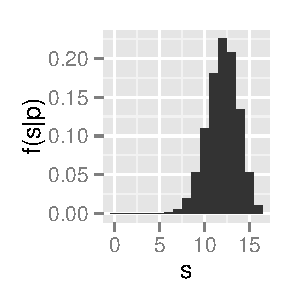
\includegraphics[width=0.25\textwidth]{figs/smallfig-binom}};}
\uncover<4-5>{%
\node at (-4.5,0) {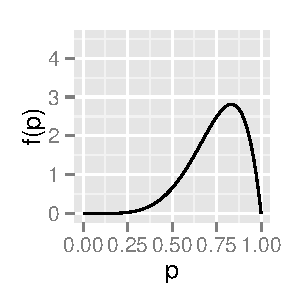
\includegraphics[width=0.25\textwidth]{figs/smallfig-prior}};}
\uncover<5>{%
\node at ( 3.5,0) {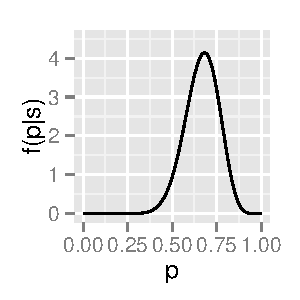
\includegraphics[width=0.25\textwidth]{figs/smallfig-posterior}};}
\end{tikzpicture}
\end{frame}

\begin{frame}{Bayesian Inference with Credal Sets}
\begin{block}{Bayesian inference with sets of priors}
\uncover<1->{%
set of priors $\MZ$ $\to$ sets of posteriors $\MN$\\
by updating element by element }\\[1ex]
\uncover<2->{%
the Generalized Bayes Rule \parencite[GBR,][]{1991:walley}\\
ensures \emph{coherence} (a consistency property) }\\[1ex]
\uncover<3->{%
Bounds for inferences (point estimate, \ldots) by min / max over $\MN$}
\end{block}
\uncover<4->{%
this offers advantages over usual Bayesian inference in case of}
\begin{itemize}
\item<4-> prior ignorance / weakly informative priors
\item<5-> prior-data conflict
\end{itemize}
\end{frame}

\begin{frame}{`Non-informative' Priors}
  How to construct a prior if we do not have a lot of information?
\pause
  \begin{block}{Laplace: Principle of Indifference}
    Use the uniform distribution.
  \end{block}
\pause
  Obvious issue: this depends on the parametrisation!
\pause
  \begin{exampleblock}{Example}
    An object of 1kg has uncertain volume $V$ between $1\ell$ and $2\ell$.
    \begin{itemize}
    \item<5-> Uniform distribution over volume $V$ $\implies$ $E(V)=1.5\ell$.
    \item<6-> Uniform distribution over density $\rho=1/V$ $\implies$ \\
      $E(V)=E(1/\rho)=\int_{0.5}^1 2/\rho\, \dd\rho=2(\ln 1-\ln 0.5)=1.39\ell$
    \end{itemize}
  \end{exampleblock}
\uncover<7->{%
  \alert{The uniform distribution does not really model prior ignorance!}}
\uncover<8->{%
  {\small (Jeffreys prior is transformation-invariant,\\ but depends on the sample space and can break decision making!)}}
\end{frame}

\begin{frame}{Prior Ignorance via Sets of Probabilities}
   How to construct a prior if we do not have a lot of information?
\pause
  \begin{block}{Boole: Probability Bounding}
    Use the set of all probability distributions (\alert{vacuous model}).
  \end{block}
  Results no longer depend on parametrisation!
\pause
  \begin{exampleblock}{Example}
    An object of 1kg has uncertain volume $V$ between $1\ell$ and $2\ell$.
    \begin{itemize}
    \item<4-> Set of all distributions over volume $V$ $\implies$ $E(V)\in[1,2]$.
    \item<5-> Set of all distributions over density $\rho=1/V$\\
      \hspace*{31ex} $\implies$ $E(V)=E(1/\rho)\in[1,2]$
    \end{itemize}
  \end{exampleblock}
\vspace*{8.25ex}
\end{frame}

\begin{frame}{Prior Ignorance via Sets of Probabilities}
  \begin{theorem}
    The set of posterior distributions
    resulting from a vacuous set of prior distributions
    is again vacuous,
    regardless of the likelihood.
  \end{theorem}
  \alert{We can never learn anything when starting from a vacuous set of priors!}
\pause
  \begin{alertblock}{Solution: Near-Vacuous Sets of Priors}
    Only insist that the prior predictive, or other classes of inferences,\\ are vacuous.
  \end{alertblock}
  This can be done using sets of conjugate priors\\
  (\cite{1996:walley::idm}; Benavoli and Zaffalon \cite*{2012:benavolizaffalon,2015:benavolizaffalon}).
\end{frame}

\begin{frame}{Example: Imprecise Beta Model (IBM)}
\begin{itemize}[<+->]
\item Bernoulli observations: 0/1 observations (failure/success)
\item given: $s$ successes in $n$ i.i.d.\ trials and strong prior information
\item we are, e.g., interested in probability for success in next trial
\end{itemize}
\vspace*{-2ex}
\begin{tikzpicture}
\uncover<4>{%
\node {\parbox{\textwidth}{%
\begin{block}{Beta-Binomial Model}
\begin{tabular}{r|lcll}
data :           & $s \mid p$        & $\sim$ & $\bin(n,p)$   \\ %[0.5ex]
conjugate prior: & $p \mid \az, \bz$ & $\sim$ & $\be(\az,\, \bz)$ & \phantom{$\be(\nzg, \yzr)$} \rule{0ex}{2.5ex}\\[0.5ex]
\cline{1-4}
posterior:       & $p \mid \an, \bn$ & $\sim$ & $\be(\an,\, \bn)$ & \phantom{$\be(\nng, \ynr)$} \rule{0ex}{2.5ex}
%\quad ($\frac{\tau(\x)}{n} = \frac{s}{n}$)\rule{0ex}{2.5ex}
\end{tabular}
\end{block}}};}
\uncover<5->{%
\node {\parbox{\textwidth}{%
\begin{block}{Beta-Binomial Model}
\begin{tabular}{r|lcll}
data :           & $s \mid p$        & $\sim$ & $\bin(n,p)$   \\ %[0.5ex]
conjugate prior: & $p \mid \az, \bz$ & $\sim$ & \cancel{$\be(\az,\, \bz)$} & $\be(\nzg, \yzr)$ \rule{0ex}{2.5ex} \\[0.5ex]
\cline{1-4}
posterior:       & $p \mid \an, \bn$ & $\sim$ & \cancel{$\be(\an,\, \bn)$} & $\be(\nng, \ynr)$ \rule{0ex}{2.5ex}
%\quad ($\frac{\tau(\x)}{n} = \frac{s}{n}$)\rule{0ex}{2.5ex}
\end{tabular}
\end{block}}};}
\end{tikzpicture}
%where $s$ = number of successes in the $n$ observed trials\\[1ex] %}
\uncover<6->{%
Vary hyperparameters $(\nzg, \yzr)$ in a set $\PZc$ \play\ set of priors $\MZ$\\[1ex] }
\uncover<7->{%
Set of posteriors $\MN$ via $\PNc = \big\{(\nng,\ynr) \colon (\nzg,\yzr) \in \PZc \big\}$\\[1ex]
Bounds for inferences (point estimate, \ldots) by min/max over $\PZc$. }
\end{frame}

\begin{frame}{Reparametrisation of the Beta Distribution}
\uncover<1->{\play\ reparametrisation helps to understand the parameter update:\\} %effect of prior-data conflict:\\}
\begin{tikzpicture}
[pfeil/.style={-latex', line width=1mm, color=tuered, shorten <=1mm},
 cyanrand/.style={rounded corners, text centered, draw=tuecyan!50, inner sep=1mm, line width=0.7mm},
 redbrace/.style={draw=tuered, decoration=brace, decorate, line width=0.8mm},
 redbox/.style={text centered, draw=tuered, inner sep=1.5mm, line width=1mm, minimum width=0.75\textwidth}]
\uncover<1->{%
\node at (0,0.2) {\parbox[c]{\textwidth}{%
\begin{align*}
\nzg &= \az + \bz\,,
&
\yzr &= \frac{\az}{\az + \bz}\,, \quad \text{which are updated as}\\%[1.5ex]
%\\
%\end{align*}
%\intertext{%
%such that
%$\lambda \sim \ig(\nz+1,\nz\yz)$ and $\lambda\mid\mbf{t} \sim \ig(\nell+1,\nell\yell)$,
%where}%
%\begin{align*}
\nng &= \nzg + n\,, 
&
\ynr &=  \frac{\nzg}{\nzg + n} \, \yzr + \frac{n}{\nzg + n} \cdot \frac{s}{n}
\end{align*}
}};}
\uncover<2->{%
\node[cyanrand] (yz) at (-0.9,-1.9) {$\yzr = \E[p]$};
\draw [pfeil] (yz.north east) to [out= 30,in=260] ( 0.9,-0.65);
\draw [pfeil] (yz.north west) to [out=130,in=240] (-1.7,0.4);}
\uncover<3->{%
\node[cyanrand] (yn) at ( 1.4,-1.9) {$\ynr = \E[p \mid s]$};
\draw [pfeil] (yn.north)      to [out=130,in=280] (-1.4,-0.65);}
\uncover<4->{%
\node[cyanrand] (ml) at ( 4.3,-1.9) {ML estimator $\hat{p}$};
\draw [pfeil] (ml.north)      to [out=100,in=330] (3.6,-0.65);}
\uncover<5->{%
\node[cyanrand] (nz) at (-4  ,-1.9) {$\nzg =$ pseudocounts};
\draw [pfeil] (nz.north)      to [out=90,in=270] (-4.0,-0.65);
\draw [pfeil] (nz.north west) to [out=95,in=240] (-5.2, 0.5);}
\uncover<6->{%
\node[redbox] at (0,-2.8) {$\E[p \mid s] = \ynr$ is a weighted average of $\E[p]$ and $\hat{p}$!};}
\uncover<7->{%
\node[redbox] at (0,-4.0) {$\V[p \mid s] = \dfrac{\ynr (1-\ynr)}{\nng + 1}$ decreases with $n$!};}
\end{tikzpicture}
\end{frame}

\begin{frame}{Beta-Binomial Model (BBM)}
\hspace*{-12ex}
\begin{columns}%[T]
\begin{column}{0.55\textwidth}
\begin{tikzpicture}
\pgftransformscale{0.025}
\uncover<1>{
% Created by tikzDevice version 0.10.1 on 2016-12-05 21:56:13
% !TEX encoding = UTF-8 Unicode
\definecolor{fillColor}{RGB}{255,255,255}
\path[use as bounding box,fill=fillColor,fill opacity=0.00] (0,0) rectangle (252.94,289.08);
\begin{scope}
\path[clip] (  0.00,  0.00) rectangle (252.94,289.08);
\definecolor{drawColor}{RGB}{0,0,0}

\path[draw=drawColor,line width= 0.4pt,line join=round,line cap=round] ( 85.06, 49.20) -- (211.08, 49.20);

\path[draw=drawColor,line width= 0.4pt,line join=round,line cap=round] ( 85.06, 49.20) -- ( 85.06, 43.20);

\path[draw=drawColor,line width= 0.4pt,line join=round,line cap=round] (127.07, 49.20) -- (127.07, 43.20);

\path[draw=drawColor,line width= 0.4pt,line join=round,line cap=round] (169.07, 49.20) -- (169.07, 43.20);

\path[draw=drawColor,line width= 0.4pt,line join=round,line cap=round] (211.08, 49.20) -- (211.08, 43.20);

\node[text=drawColor,anchor=base,inner sep=0pt, outer sep=0pt, scale=  1.00] at ( 85.06, 27.60) {0};

\node[text=drawColor,anchor=base,inner sep=0pt, outer sep=0pt, scale=  1.00] at (127.07, 27.60) {5};

\node[text=drawColor,anchor=base,inner sep=0pt, outer sep=0pt, scale=  1.00] at (169.07, 27.60) {10};

\node[text=drawColor,anchor=base,inner sep=0pt, outer sep=0pt, scale=  1.00] at (211.08, 27.60) {15};

\path[draw=drawColor,line width= 0.4pt,line join=round,line cap=round] ( 61.20, 55.82) -- ( 61.20,221.26);

\path[draw=drawColor,line width= 0.4pt,line join=round,line cap=round] ( 61.20, 55.82) -- ( 55.20, 55.82);

\path[draw=drawColor,line width= 0.4pt,line join=round,line cap=round] ( 61.20, 88.91) -- ( 55.20, 88.91);

\path[draw=drawColor,line width= 0.4pt,line join=round,line cap=round] ( 61.20,122.00) -- ( 55.20,122.00);

\path[draw=drawColor,line width= 0.4pt,line join=round,line cap=round] ( 61.20,155.08) -- ( 55.20,155.08);

\path[draw=drawColor,line width= 0.4pt,line join=round,line cap=round] ( 61.20,188.17) -- ( 55.20,188.17);

\path[draw=drawColor,line width= 0.4pt,line join=round,line cap=round] ( 61.20,221.26) -- ( 55.20,221.26);

\node[text=drawColor,rotate= 90.00,anchor=base,inner sep=0pt, outer sep=0pt, scale=  1.00] at ( 46.80, 55.82) {0.0};

\node[text=drawColor,rotate= 90.00,anchor=base,inner sep=0pt, outer sep=0pt, scale=  1.00] at ( 46.80, 88.91) {0.2};

\node[text=drawColor,rotate= 90.00,anchor=base,inner sep=0pt, outer sep=0pt, scale=  1.00] at ( 46.80,122.00) {0.4};

\node[text=drawColor,rotate= 90.00,anchor=base,inner sep=0pt, outer sep=0pt, scale=  1.00] at ( 46.80,155.08) {0.6};

\node[text=drawColor,rotate= 90.00,anchor=base,inner sep=0pt, outer sep=0pt, scale=  1.00] at ( 46.80,188.17) {0.8};

\node[text=drawColor,rotate= 90.00,anchor=base,inner sep=0pt, outer sep=0pt, scale=  1.00] at ( 46.80,221.26) {1.0};

\path[draw=drawColor,line width= 0.4pt,line join=round,line cap=round] ( 61.20, 49.20) --
	(251.74, 49.20) --
	(251.74,227.88) --
	( 61.20,227.88) --
	( 61.20, 49.20);
\end{scope}
\begin{scope}
\path[clip] ( 61.20, 49.20) rectangle (251.74,227.88);
\definecolor{drawColor}{RGB}{0,0,0}
\definecolor{fillColor}{RGB}{190,190,190}

\path[draw=drawColor,line width= 0.4pt,line join=round,line cap=round,fill=fillColor] (101.86,138.54) --
	(101.86,138.54) --
	(101.86,138.54) --
	(101.86,138.54) --
	cycle;
\end{scope}
\begin{scope}
\path[clip] (  0.00,  0.00) rectangle (252.94,289.08);
\definecolor{drawColor}{RGB}{0,0,0}

\node[text=drawColor,anchor=base,inner sep=0pt, outer sep=0pt, scale=  1.00] at (156.47,  3.60) {$\nzg$ resp. $\nng$};

\node[text=drawColor,rotate= 90.00,anchor=base,inner sep=0pt, outer sep=0pt, scale=  1.00] at ( 22.80,138.54) {$\yzr$ resp. $\ynr$};
\end{scope}
\begin{scope}
\path[clip] ( 61.20, 49.20) rectangle (251.74,227.88);
\definecolor{drawColor}{RGB}{0,0,0}
\definecolor{fillColor}{RGB}{0,0,0}

\path[draw=drawColor,line width= 0.4pt,line join=round,line cap=round,fill=fillColor] (101.86,138.54) circle (  2.25);
\end{scope}

}
\uncover<2>{
% Created by tikzDevice version 0.10.1 on 2016-12-05 21:56:18
% !TEX encoding = UTF-8 Unicode
\definecolor{fillColor}{RGB}{255,255,255}
\path[use as bounding box,fill=fillColor,fill opacity=0.00] (0,0) rectangle (252.94,289.08);
\begin{scope}
\path[clip] (  0.00,  0.00) rectangle (252.94,289.08);
\definecolor{drawColor}{RGB}{0,0,0}

\path[draw=drawColor,line width= 0.4pt,line join=round,line cap=round] ( 85.06, 49.20) -- (211.08, 49.20);

\path[draw=drawColor,line width= 0.4pt,line join=round,line cap=round] ( 85.06, 49.20) -- ( 85.06, 43.20);

\path[draw=drawColor,line width= 0.4pt,line join=round,line cap=round] (127.07, 49.20) -- (127.07, 43.20);

\path[draw=drawColor,line width= 0.4pt,line join=round,line cap=round] (169.07, 49.20) -- (169.07, 43.20);

\path[draw=drawColor,line width= 0.4pt,line join=round,line cap=round] (211.08, 49.20) -- (211.08, 43.20);

\node[text=drawColor,anchor=base,inner sep=0pt, outer sep=0pt, scale=  1.00] at ( 85.06, 27.60) {0};

\node[text=drawColor,anchor=base,inner sep=0pt, outer sep=0pt, scale=  1.00] at (127.07, 27.60) {5};

\node[text=drawColor,anchor=base,inner sep=0pt, outer sep=0pt, scale=  1.00] at (169.07, 27.60) {10};

\node[text=drawColor,anchor=base,inner sep=0pt, outer sep=0pt, scale=  1.00] at (211.08, 27.60) {15};

\path[draw=drawColor,line width= 0.4pt,line join=round,line cap=round] ( 61.20, 55.82) -- ( 61.20,221.26);

\path[draw=drawColor,line width= 0.4pt,line join=round,line cap=round] ( 61.20, 55.82) -- ( 55.20, 55.82);

\path[draw=drawColor,line width= 0.4pt,line join=round,line cap=round] ( 61.20, 88.91) -- ( 55.20, 88.91);

\path[draw=drawColor,line width= 0.4pt,line join=round,line cap=round] ( 61.20,122.00) -- ( 55.20,122.00);

\path[draw=drawColor,line width= 0.4pt,line join=round,line cap=round] ( 61.20,155.08) -- ( 55.20,155.08);

\path[draw=drawColor,line width= 0.4pt,line join=round,line cap=round] ( 61.20,188.17) -- ( 55.20,188.17);

\path[draw=drawColor,line width= 0.4pt,line join=round,line cap=round] ( 61.20,221.26) -- ( 55.20,221.26);

\node[text=drawColor,rotate= 90.00,anchor=base,inner sep=0pt, outer sep=0pt, scale=  1.00] at ( 46.80, 55.82) {0.0};

\node[text=drawColor,rotate= 90.00,anchor=base,inner sep=0pt, outer sep=0pt, scale=  1.00] at ( 46.80, 88.91) {0.2};

\node[text=drawColor,rotate= 90.00,anchor=base,inner sep=0pt, outer sep=0pt, scale=  1.00] at ( 46.80,122.00) {0.4};

\node[text=drawColor,rotate= 90.00,anchor=base,inner sep=0pt, outer sep=0pt, scale=  1.00] at ( 46.80,155.08) {0.6};

\node[text=drawColor,rotate= 90.00,anchor=base,inner sep=0pt, outer sep=0pt, scale=  1.00] at ( 46.80,188.17) {0.8};

\node[text=drawColor,rotate= 90.00,anchor=base,inner sep=0pt, outer sep=0pt, scale=  1.00] at ( 46.80,221.26) {1.0};

\path[draw=drawColor,line width= 0.4pt,line join=round,line cap=round] ( 61.20, 49.20) --
	(251.74, 49.20) --
	(251.74,227.88) --
	( 61.20,227.88) --
	( 61.20, 49.20);
\end{scope}
\begin{scope}
\path[clip] ( 61.20, 49.20) rectangle (251.74,227.88);
\definecolor{drawColor}{RGB}{0,0,0}
\definecolor{fillColor}{RGB}{190,190,190}

\path[draw=drawColor,line width= 0.4pt,line join=round,line cap=round,fill=fillColor] (101.86,138.54) --
	(101.86,138.54) --
	(101.86,138.54) --
	(101.86,138.54) --
	cycle;

\path[draw=drawColor,line width= 0.4pt,line join=round,line cap=round,fill=fillColor] (236.29,175.31) --
	(236.29,175.31) --
	(236.29,175.31) --
	(236.29,175.31) --
	(236.29,175.31) --
	(236.29,175.31) --
	(236.29,175.31) --
	(236.29,175.31) --
	(236.29,175.31) --
	(236.29,175.31) --
	(236.29,175.31) --
	(236.29,175.31) --
	(236.29,175.31) --
	(236.29,175.31) --
	(236.29,175.31) --
	(236.29,175.31) --
	(236.29,175.31) --
	(236.29,175.31) --
	(236.29,175.31) --
	(236.29,175.31) --
	(236.29,175.31) --
	(236.29,175.31) --
	(236.29,175.31) --
	(236.29,175.31) --
	(236.29,175.31) --
	(236.29,175.31) --
	(236.29,175.31) --
	(236.29,175.31) --
	(236.29,175.31) --
	(236.29,175.31) --
	(236.29,175.31) --
	(236.29,175.31) --
	(236.29,175.31) --
	(236.29,175.31) --
	(236.29,175.31) --
	(236.29,175.31) --
	(236.29,175.31) --
	(236.29,175.31) --
	(236.29,175.31) --
	(236.29,175.31) --
	(236.29,175.31) --
	(236.29,175.31) --
	(236.29,175.31) --
	(236.29,175.31) --
	(236.29,175.31) --
	(236.29,175.31) --
	(236.29,175.31) --
	(236.29,175.31) --
	(236.29,175.31) --
	(236.29,175.31) --
	(236.29,175.31) --
	(236.29,175.31) --
	(236.29,175.31) --
	(236.29,175.31) --
	(236.29,175.31) --
	(236.29,175.31) --
	(236.29,175.31) --
	(236.29,175.31) --
	(236.29,175.31) --
	(236.29,175.31) --
	(236.29,175.31) --
	(236.29,175.31) --
	(236.29,175.31) --
	(236.29,175.31) --
	(236.29,175.31) --
	(236.29,175.31) --
	(236.29,175.31) --
	(236.29,175.31) --
	(236.29,175.31) --
	(236.29,175.31) --
	(236.29,175.31) --
	(236.29,175.31) --
	(236.29,175.31) --
	(236.29,175.31) --
	(236.29,175.31) --
	(236.29,175.31) --
	(236.29,175.31) --
	(236.29,175.31) --
	(236.29,175.31) --
	(236.29,175.31) --
	(236.29,175.31) --
	(236.29,175.31) --
	(236.29,175.31) --
	(236.29,175.31) --
	(236.29,175.31) --
	(236.29,175.31) --
	(236.29,175.31) --
	(236.29,175.31) --
	(236.29,175.31) --
	(236.29,175.31) --
	(236.29,175.31) --
	(236.29,175.31) --
	(236.29,175.31) --
	(236.29,175.31) --
	(236.29,175.31) --
	(236.29,175.31) --
	(236.29,175.31) --
	(236.29,175.31) --
	(236.29,175.31) --
	(236.29,175.31) --
	(236.29,175.31) --
	(236.29,175.31) --
	(236.29,175.31) --
	(236.29,175.31) --
	(236.29,175.31) --
	(236.29,175.31) --
	(236.29,175.31) --
	(236.29,175.31) --
	(236.29,175.31) --
	(236.29,175.31) --
	(236.29,175.31) --
	(236.29,175.31) --
	(236.29,175.31) --
	(236.29,175.31) --
	(236.29,175.31) --
	(236.29,175.31) --
	(236.29,175.31) --
	(236.29,175.31) --
	(236.29,175.31) --
	(236.29,175.31) --
	(236.29,175.31) --
	(236.29,175.31) --
	(236.29,175.31) --
	(236.29,175.31) --
	(236.29,175.31) --
	(236.29,175.31) --
	(236.29,175.31) --
	(236.29,175.31) --
	(236.29,175.31) --
	(236.29,175.31) --
	(236.29,175.31) --
	(236.29,175.31) --
	(236.29,175.31) --
	(236.29,175.31) --
	(236.29,175.31) --
	(236.29,175.31) --
	(236.29,175.31) --
	(236.29,175.31) --
	(236.29,175.31) --
	(236.29,175.31) --
	(236.29,175.31) --
	(236.29,175.31) --
	(236.29,175.31) --
	(236.29,175.31) --
	(236.29,175.31) --
	(236.29,175.31) --
	(236.29,175.31) --
	(236.29,175.31) --
	(236.29,175.31) --
	(236.29,175.31) --
	(236.29,175.31) --
	(236.29,175.31) --
	(236.29,175.31) --
	(236.29,175.31) --
	(236.29,175.31) --
	(236.29,175.31) --
	(236.29,175.31) --
	(236.29,175.31) --
	(236.29,175.31) --
	(236.29,175.31) --
	(236.29,175.31) --
	(236.29,175.31) --
	(236.29,175.31) --
	(236.29,175.31) --
	(236.29,175.31) --
	(236.29,175.31) --
	(236.29,175.31) --
	(236.29,175.31) --
	(236.29,175.31) --
	(236.29,175.31) --
	(236.29,175.31) --
	(236.29,175.31) --
	(236.29,175.31) --
	(236.29,175.31) --
	(236.29,175.31) --
	(236.29,175.31) --
	(236.29,175.31) --
	(236.29,175.31) --
	(236.29,175.31) --
	(236.29,175.31) --
	(236.29,175.31) --
	(236.29,175.31) --
	(236.29,175.31) --
	(236.29,175.31) --
	(236.29,175.31) --
	(236.29,175.31) --
	(236.29,175.31) --
	(236.29,175.31) --
	(236.29,175.31) --
	(236.29,175.31) --
	(236.29,175.31) --
	(236.29,175.31) --
	(236.29,175.31) --
	(236.29,175.31) --
	(236.29,175.31) --
	(236.29,175.31) --
	(236.29,175.31) --
	(236.29,175.31) --
	(236.29,175.31) --
	(236.29,175.31) --
	cycle;
\end{scope}
\begin{scope}
\path[clip] (  0.00,  0.00) rectangle (252.94,289.08);
\definecolor{drawColor}{RGB}{0,0,0}

\node[text=drawColor,anchor=base,inner sep=0pt, outer sep=0pt, scale=  1.00] at (156.47,  3.60) {$\nzg$ resp. $\nng$};

\node[text=drawColor,rotate= 90.00,anchor=base,inner sep=0pt, outer sep=0pt, scale=  1.00] at ( 22.80,138.54) {$\yzr$ resp. $\ynr$};
\end{scope}
\begin{scope}
\path[clip] ( 61.20, 49.20) rectangle (251.74,227.88);
\definecolor{drawColor}{RGB}{0,0,0}
\definecolor{fillColor}{RGB}{0,0,0}

\path[draw=drawColor,line width= 0.4pt,line join=round,line cap=round,fill=fillColor] (101.86,138.54) circle (  2.25);

\path[draw=drawColor,line width= 0.4pt,line join=round,line cap=round,fill=fillColor] (236.29,175.31) circle (  2.25);
\end{scope}

\draw[-stealth,very thick] (115,142) -- (225,172) node [above,midway, sloped] {12 out of 16};
}
\uncover<3->{
% Created by tikzDevice version 0.10.1 on 2016-12-05 21:56:35
% !TEX encoding = UTF-8 Unicode
\definecolor{fillColor}{RGB}{255,255,255}
\path[use as bounding box,fill=fillColor,fill opacity=0.00] (0,0) rectangle (252.94,289.08);
\begin{scope}
\path[clip] (  0.00,  0.00) rectangle (252.94,289.08);
\definecolor{drawColor}{RGB}{0,0,0}

\path[draw=drawColor,line width= 0.4pt,line join=round,line cap=round] ( 85.06, 49.20) -- (211.08, 49.20);

\path[draw=drawColor,line width= 0.4pt,line join=round,line cap=round] ( 85.06, 49.20) -- ( 85.06, 43.20);

\path[draw=drawColor,line width= 0.4pt,line join=round,line cap=round] (127.07, 49.20) -- (127.07, 43.20);

\path[draw=drawColor,line width= 0.4pt,line join=round,line cap=round] (169.07, 49.20) -- (169.07, 43.20);

\path[draw=drawColor,line width= 0.4pt,line join=round,line cap=round] (211.08, 49.20) -- (211.08, 43.20);

\node[text=drawColor,anchor=base,inner sep=0pt, outer sep=0pt, scale=  1.00] at ( 85.06, 27.60) {0};

\node[text=drawColor,anchor=base,inner sep=0pt, outer sep=0pt, scale=  1.00] at (127.07, 27.60) {5};

\node[text=drawColor,anchor=base,inner sep=0pt, outer sep=0pt, scale=  1.00] at (169.07, 27.60) {10};

\node[text=drawColor,anchor=base,inner sep=0pt, outer sep=0pt, scale=  1.00] at (211.08, 27.60) {15};

\path[draw=drawColor,line width= 0.4pt,line join=round,line cap=round] ( 61.20, 55.82) -- ( 61.20,221.26);

\path[draw=drawColor,line width= 0.4pt,line join=round,line cap=round] ( 61.20, 55.82) -- ( 55.20, 55.82);

\path[draw=drawColor,line width= 0.4pt,line join=round,line cap=round] ( 61.20, 88.91) -- ( 55.20, 88.91);

\path[draw=drawColor,line width= 0.4pt,line join=round,line cap=round] ( 61.20,122.00) -- ( 55.20,122.00);

\path[draw=drawColor,line width= 0.4pt,line join=round,line cap=round] ( 61.20,155.08) -- ( 55.20,155.08);

\path[draw=drawColor,line width= 0.4pt,line join=round,line cap=round] ( 61.20,188.17) -- ( 55.20,188.17);

\path[draw=drawColor,line width= 0.4pt,line join=round,line cap=round] ( 61.20,221.26) -- ( 55.20,221.26);

\node[text=drawColor,rotate= 90.00,anchor=base,inner sep=0pt, outer sep=0pt, scale=  1.00] at ( 46.80, 55.82) {0.0};

\node[text=drawColor,rotate= 90.00,anchor=base,inner sep=0pt, outer sep=0pt, scale=  1.00] at ( 46.80, 88.91) {0.2};

\node[text=drawColor,rotate= 90.00,anchor=base,inner sep=0pt, outer sep=0pt, scale=  1.00] at ( 46.80,122.00) {0.4};

\node[text=drawColor,rotate= 90.00,anchor=base,inner sep=0pt, outer sep=0pt, scale=  1.00] at ( 46.80,155.08) {0.6};

\node[text=drawColor,rotate= 90.00,anchor=base,inner sep=0pt, outer sep=0pt, scale=  1.00] at ( 46.80,188.17) {0.8};

\node[text=drawColor,rotate= 90.00,anchor=base,inner sep=0pt, outer sep=0pt, scale=  1.00] at ( 46.80,221.26) {1.0};

\path[draw=drawColor,line width= 0.4pt,line join=round,line cap=round] ( 61.20, 49.20) --
	(251.74, 49.20) --
	(251.74,227.88) --
	( 61.20,227.88) --
	( 61.20, 49.20);
\end{scope}
\begin{scope}
\path[clip] ( 61.20, 49.20) rectangle (251.74,227.88);
\definecolor{drawColor}{RGB}{0,0,0}
\definecolor{fillColor}{RGB}{190,190,190}

\path[draw=drawColor,line width= 0.4pt,line join=round,line cap=round,fill=fillColor] (101.86,138.54) --
	(101.86,138.54) --
	(101.86,138.54) --
	(101.86,138.54) --
	cycle;

\path[draw=drawColor,line width= 0.4pt,line join=round,line cap=round,fill=fillColor] (236.29,175.31) --
	(236.29,175.31) --
	(236.29,175.31) --
	(236.29,175.31) --
	(236.29,175.31) --
	(236.29,175.31) --
	(236.29,175.31) --
	(236.29,175.31) --
	(236.29,175.31) --
	(236.29,175.31) --
	(236.29,175.31) --
	(236.29,175.31) --
	(236.29,175.31) --
	(236.29,175.31) --
	(236.29,175.31) --
	(236.29,175.31) --
	(236.29,175.31) --
	(236.29,175.31) --
	(236.29,175.31) --
	(236.29,175.31) --
	(236.29,175.31) --
	(236.29,175.31) --
	(236.29,175.31) --
	(236.29,175.31) --
	(236.29,175.31) --
	(236.29,175.31) --
	(236.29,175.31) --
	(236.29,175.31) --
	(236.29,175.31) --
	(236.29,175.31) --
	(236.29,175.31) --
	(236.29,175.31) --
	(236.29,175.31) --
	(236.29,175.31) --
	(236.29,175.31) --
	(236.29,175.31) --
	(236.29,175.31) --
	(236.29,175.31) --
	(236.29,175.31) --
	(236.29,175.31) --
	(236.29,175.31) --
	(236.29,175.31) --
	(236.29,175.31) --
	(236.29,175.31) --
	(236.29,175.31) --
	(236.29,175.31) --
	(236.29,175.31) --
	(236.29,175.31) --
	(236.29,175.31) --
	(236.29,175.31) --
	(236.29,175.31) --
	(236.29,175.31) --
	(236.29,175.31) --
	(236.29,175.31) --
	(236.29,175.31) --
	(236.29,175.31) --
	(236.29,175.31) --
	(236.29,175.31) --
	(236.29,175.31) --
	(236.29,175.31) --
	(236.29,175.31) --
	(236.29,175.31) --
	(236.29,175.31) --
	(236.29,175.31) --
	(236.29,175.31) --
	(236.29,175.31) --
	(236.29,175.31) --
	(236.29,175.31) --
	(236.29,175.31) --
	(236.29,175.31) --
	(236.29,175.31) --
	(236.29,175.31) --
	(236.29,175.31) --
	(236.29,175.31) --
	(236.29,175.31) --
	(236.29,175.31) --
	(236.29,175.31) --
	(236.29,175.31) --
	(236.29,175.31) --
	(236.29,175.31) --
	(236.29,175.31) --
	(236.29,175.31) --
	(236.29,175.31) --
	(236.29,175.31) --
	(236.29,175.31) --
	(236.29,175.31) --
	(236.29,175.31) --
	(236.29,175.31) --
	(236.29,175.31) --
	(236.29,175.31) --
	(236.29,175.31) --
	(236.29,175.31) --
	(236.29,175.31) --
	(236.29,175.31) --
	(236.29,175.31) --
	(236.29,175.31) --
	(236.29,175.31) --
	(236.29,175.31) --
	(236.29,175.31) --
	(236.29,175.31) --
	(236.29,175.31) --
	(236.29,175.31) --
	(236.29,175.31) --
	(236.29,175.31) --
	(236.29,175.31) --
	(236.29,175.31) --
	(236.29,175.31) --
	(236.29,175.31) --
	(236.29,175.31) --
	(236.29,175.31) --
	(236.29,175.31) --
	(236.29,175.31) --
	(236.29,175.31) --
	(236.29,175.31) --
	(236.29,175.31) --
	(236.29,175.31) --
	(236.29,175.31) --
	(236.29,175.31) --
	(236.29,175.31) --
	(236.29,175.31) --
	(236.29,175.31) --
	(236.29,175.31) --
	(236.29,175.31) --
	(236.29,175.31) --
	(236.29,175.31) --
	(236.29,175.31) --
	(236.29,175.31) --
	(236.29,175.31) --
	(236.29,175.31) --
	(236.29,175.31) --
	(236.29,175.31) --
	(236.29,175.31) --
	(236.29,175.31) --
	(236.29,175.31) --
	(236.29,175.31) --
	(236.29,175.31) --
	(236.29,175.31) --
	(236.29,175.31) --
	(236.29,175.31) --
	(236.29,175.31) --
	(236.29,175.31) --
	(236.29,175.31) --
	(236.29,175.31) --
	(236.29,175.31) --
	(236.29,175.31) --
	(236.29,175.31) --
	(236.29,175.31) --
	(236.29,175.31) --
	(236.29,175.31) --
	(236.29,175.31) --
	(236.29,175.31) --
	(236.29,175.31) --
	(236.29,175.31) --
	(236.29,175.31) --
	(236.29,175.31) --
	(236.29,175.31) --
	(236.29,175.31) --
	(236.29,175.31) --
	(236.29,175.31) --
	(236.29,175.31) --
	(236.29,175.31) --
	(236.29,175.31) --
	(236.29,175.31) --
	(236.29,175.31) --
	(236.29,175.31) --
	(236.29,175.31) --
	(236.29,175.31) --
	(236.29,175.31) --
	(236.29,175.31) --
	(236.29,175.31) --
	(236.29,175.31) --
	(236.29,175.31) --
	(236.29,175.31) --
	(236.29,175.31) --
	(236.29,175.31) --
	(236.29,175.31) --
	(236.29,175.31) --
	(236.29,175.31) --
	(236.29,175.31) --
	(236.29,175.31) --
	(236.29,175.31) --
	(236.29,175.31) --
	(236.29,175.31) --
	(236.29,175.31) --
	(236.29,175.31) --
	(236.29,175.31) --
	(236.29,175.31) --
	(236.29,175.31) --
	(236.29,175.31) --
	(236.29,175.31) --
	(236.29,175.31) --
	(236.29,175.31) --
	(236.29,175.31) --
	(236.29,175.31) --
	(236.29,175.31) --
	(236.29,175.31) --
	(236.29,175.31) --
	(236.29,175.31) --
	(236.29,175.31) --
	(236.29,175.31) --
	cycle;
\end{scope}
\begin{scope}
\path[clip] (  0.00,  0.00) rectangle (252.94,289.08);
\definecolor{drawColor}{RGB}{0,0,0}

\node[text=drawColor,anchor=base,inner sep=0pt, outer sep=0pt, scale=  1.00] at (156.47,  3.60) {$\nzg$ resp. $\nng$};

\node[text=drawColor,rotate= 90.00,anchor=base,inner sep=0pt, outer sep=0pt, scale=  1.00] at ( 22.80,138.54) {$\yzr$ resp. $\ynr$};
\end{scope}
\begin{scope}
\path[clip] ( 61.20, 49.20) rectangle (251.74,227.88);
\definecolor{drawColor}{RGB}{190,190,190}
\definecolor{fillColor}{RGB}{190,190,190}

\path[draw=drawColor,line width= 0.4pt,line join=round,line cap=round,fill=fillColor] (101.86,138.54) circle (  2.25);

\path[draw=drawColor,line width= 0.4pt,line join=round,line cap=round,fill=fillColor] (236.29,175.31) circle (  2.25);
\definecolor{drawColor}{RGB}{0,0,0}

\path[draw=drawColor,line width= 0.9pt,line join=round,line cap=round,fill=fillColor] (101.86, 55.82) --
	(101.86, 55.82) --
	(101.86,221.26) --
	(101.86,221.26) --
	cycle;
\end{scope}

\draw[-stealth,very thick, gray] (115,142) -- (225,172) node [above,midway,sloped,gray] {12 out of 16};
}
\uncover<4->{
% Created by tikzDevice version 0.10.1 on 2016-12-05 21:56:43
% !TEX encoding = UTF-8 Unicode
\definecolor{fillColor}{RGB}{255,255,255}
\path[use as bounding box,fill=fillColor,fill opacity=0.00] (0,0) rectangle (252.94,289.08);
\begin{scope}
\path[clip] (  0.00,  0.00) rectangle (252.94,289.08);
\definecolor{drawColor}{RGB}{0,0,0}

\path[draw=drawColor,line width= 0.4pt,line join=round,line cap=round] ( 85.06, 49.20) -- (211.08, 49.20);

\path[draw=drawColor,line width= 0.4pt,line join=round,line cap=round] ( 85.06, 49.20) -- ( 85.06, 43.20);

\path[draw=drawColor,line width= 0.4pt,line join=round,line cap=round] (127.07, 49.20) -- (127.07, 43.20);

\path[draw=drawColor,line width= 0.4pt,line join=round,line cap=round] (169.07, 49.20) -- (169.07, 43.20);

\path[draw=drawColor,line width= 0.4pt,line join=round,line cap=round] (211.08, 49.20) -- (211.08, 43.20);

\node[text=drawColor,anchor=base,inner sep=0pt, outer sep=0pt, scale=  1.00] at ( 85.06, 27.60) {0};

\node[text=drawColor,anchor=base,inner sep=0pt, outer sep=0pt, scale=  1.00] at (127.07, 27.60) {5};

\node[text=drawColor,anchor=base,inner sep=0pt, outer sep=0pt, scale=  1.00] at (169.07, 27.60) {10};

\node[text=drawColor,anchor=base,inner sep=0pt, outer sep=0pt, scale=  1.00] at (211.08, 27.60) {15};

\path[draw=drawColor,line width= 0.4pt,line join=round,line cap=round] ( 61.20, 55.82) -- ( 61.20,221.26);

\path[draw=drawColor,line width= 0.4pt,line join=round,line cap=round] ( 61.20, 55.82) -- ( 55.20, 55.82);

\path[draw=drawColor,line width= 0.4pt,line join=round,line cap=round] ( 61.20, 88.91) -- ( 55.20, 88.91);

\path[draw=drawColor,line width= 0.4pt,line join=round,line cap=round] ( 61.20,122.00) -- ( 55.20,122.00);

\path[draw=drawColor,line width= 0.4pt,line join=round,line cap=round] ( 61.20,155.08) -- ( 55.20,155.08);

\path[draw=drawColor,line width= 0.4pt,line join=round,line cap=round] ( 61.20,188.17) -- ( 55.20,188.17);

\path[draw=drawColor,line width= 0.4pt,line join=round,line cap=round] ( 61.20,221.26) -- ( 55.20,221.26);

\node[text=drawColor,rotate= 90.00,anchor=base,inner sep=0pt, outer sep=0pt, scale=  1.00] at ( 46.80, 55.82) {0.0};

\node[text=drawColor,rotate= 90.00,anchor=base,inner sep=0pt, outer sep=0pt, scale=  1.00] at ( 46.80, 88.91) {0.2};

\node[text=drawColor,rotate= 90.00,anchor=base,inner sep=0pt, outer sep=0pt, scale=  1.00] at ( 46.80,122.00) {0.4};

\node[text=drawColor,rotate= 90.00,anchor=base,inner sep=0pt, outer sep=0pt, scale=  1.00] at ( 46.80,155.08) {0.6};

\node[text=drawColor,rotate= 90.00,anchor=base,inner sep=0pt, outer sep=0pt, scale=  1.00] at ( 46.80,188.17) {0.8};

\node[text=drawColor,rotate= 90.00,anchor=base,inner sep=0pt, outer sep=0pt, scale=  1.00] at ( 46.80,221.26) {1.0};

\path[draw=drawColor,line width= 0.4pt,line join=round,line cap=round] ( 61.20, 49.20) --
	(251.74, 49.20) --
	(251.74,227.88) --
	( 61.20,227.88) --
	( 61.20, 49.20);
\end{scope}
\begin{scope}
\path[clip] ( 61.20, 49.20) rectangle (251.74,227.88);
\definecolor{drawColor}{RGB}{0,0,0}
\definecolor{fillColor}{RGB}{190,190,190}

\path[draw=drawColor,line width= 0.4pt,line join=round,line cap=round,fill=fillColor] (101.86,138.54) --
	(101.86,138.54) --
	(101.86,138.54) --
	(101.86,138.54) --
	cycle;

\path[draw=drawColor,line width= 0.4pt,line join=round,line cap=round,fill=fillColor] (236.29,175.31) --
	(236.29,175.31) --
	(236.29,175.31) --
	(236.29,175.31) --
	(236.29,175.31) --
	(236.29,175.31) --
	(236.29,175.31) --
	(236.29,175.31) --
	(236.29,175.31) --
	(236.29,175.31) --
	(236.29,175.31) --
	(236.29,175.31) --
	(236.29,175.31) --
	(236.29,175.31) --
	(236.29,175.31) --
	(236.29,175.31) --
	(236.29,175.31) --
	(236.29,175.31) --
	(236.29,175.31) --
	(236.29,175.31) --
	(236.29,175.31) --
	(236.29,175.31) --
	(236.29,175.31) --
	(236.29,175.31) --
	(236.29,175.31) --
	(236.29,175.31) --
	(236.29,175.31) --
	(236.29,175.31) --
	(236.29,175.31) --
	(236.29,175.31) --
	(236.29,175.31) --
	(236.29,175.31) --
	(236.29,175.31) --
	(236.29,175.31) --
	(236.29,175.31) --
	(236.29,175.31) --
	(236.29,175.31) --
	(236.29,175.31) --
	(236.29,175.31) --
	(236.29,175.31) --
	(236.29,175.31) --
	(236.29,175.31) --
	(236.29,175.31) --
	(236.29,175.31) --
	(236.29,175.31) --
	(236.29,175.31) --
	(236.29,175.31) --
	(236.29,175.31) --
	(236.29,175.31) --
	(236.29,175.31) --
	(236.29,175.31) --
	(236.29,175.31) --
	(236.29,175.31) --
	(236.29,175.31) --
	(236.29,175.31) --
	(236.29,175.31) --
	(236.29,175.31) --
	(236.29,175.31) --
	(236.29,175.31) --
	(236.29,175.31) --
	(236.29,175.31) --
	(236.29,175.31) --
	(236.29,175.31) --
	(236.29,175.31) --
	(236.29,175.31) --
	(236.29,175.31) --
	(236.29,175.31) --
	(236.29,175.31) --
	(236.29,175.31) --
	(236.29,175.31) --
	(236.29,175.31) --
	(236.29,175.31) --
	(236.29,175.31) --
	(236.29,175.31) --
	(236.29,175.31) --
	(236.29,175.31) --
	(236.29,175.31) --
	(236.29,175.31) --
	(236.29,175.31) --
	(236.29,175.31) --
	(236.29,175.31) --
	(236.29,175.31) --
	(236.29,175.31) --
	(236.29,175.31) --
	(236.29,175.31) --
	(236.29,175.31) --
	(236.29,175.31) --
	(236.29,175.31) --
	(236.29,175.31) --
	(236.29,175.31) --
	(236.29,175.31) --
	(236.29,175.31) --
	(236.29,175.31) --
	(236.29,175.31) --
	(236.29,175.31) --
	(236.29,175.31) --
	(236.29,175.31) --
	(236.29,175.31) --
	(236.29,175.31) --
	(236.29,175.31) --
	(236.29,175.31) --
	(236.29,175.31) --
	(236.29,175.31) --
	(236.29,175.31) --
	(236.29,175.31) --
	(236.29,175.31) --
	(236.29,175.31) --
	(236.29,175.31) --
	(236.29,175.31) --
	(236.29,175.31) --
	(236.29,175.31) --
	(236.29,175.31) --
	(236.29,175.31) --
	(236.29,175.31) --
	(236.29,175.31) --
	(236.29,175.31) --
	(236.29,175.31) --
	(236.29,175.31) --
	(236.29,175.31) --
	(236.29,175.31) --
	(236.29,175.31) --
	(236.29,175.31) --
	(236.29,175.31) --
	(236.29,175.31) --
	(236.29,175.31) --
	(236.29,175.31) --
	(236.29,175.31) --
	(236.29,175.31) --
	(236.29,175.31) --
	(236.29,175.31) --
	(236.29,175.31) --
	(236.29,175.31) --
	(236.29,175.31) --
	(236.29,175.31) --
	(236.29,175.31) --
	(236.29,175.31) --
	(236.29,175.31) --
	(236.29,175.31) --
	(236.29,175.31) --
	(236.29,175.31) --
	(236.29,175.31) --
	(236.29,175.31) --
	(236.29,175.31) --
	(236.29,175.31) --
	(236.29,175.31) --
	(236.29,175.31) --
	(236.29,175.31) --
	(236.29,175.31) --
	(236.29,175.31) --
	(236.29,175.31) --
	(236.29,175.31) --
	(236.29,175.31) --
	(236.29,175.31) --
	(236.29,175.31) --
	(236.29,175.31) --
	(236.29,175.31) --
	(236.29,175.31) --
	(236.29,175.31) --
	(236.29,175.31) --
	(236.29,175.31) --
	(236.29,175.31) --
	(236.29,175.31) --
	(236.29,175.31) --
	(236.29,175.31) --
	(236.29,175.31) --
	(236.29,175.31) --
	(236.29,175.31) --
	(236.29,175.31) --
	(236.29,175.31) --
	(236.29,175.31) --
	(236.29,175.31) --
	(236.29,175.31) --
	(236.29,175.31) --
	(236.29,175.31) --
	(236.29,175.31) --
	(236.29,175.31) --
	(236.29,175.31) --
	(236.29,175.31) --
	(236.29,175.31) --
	(236.29,175.31) --
	(236.29,175.31) --
	(236.29,175.31) --
	(236.29,175.31) --
	(236.29,175.31) --
	(236.29,175.31) --
	(236.29,175.31) --
	(236.29,175.31) --
	(236.29,175.31) --
	(236.29,175.31) --
	(236.29,175.31) --
	(236.29,175.31) --
	(236.29,175.31) --
	(236.29,175.31) --
	(236.29,175.31) --
	(236.29,175.31) --
	(236.29,175.31) --
	(236.29,175.31) --
	(236.29,175.31) --
	(236.29,175.31) --
	(236.29,175.31) --
	cycle;
\end{scope}
\begin{scope}
\path[clip] (  0.00,  0.00) rectangle (252.94,289.08);
\definecolor{drawColor}{RGB}{0,0,0}

\node[text=drawColor,anchor=base,inner sep=0pt, outer sep=0pt, scale=  1.00] at (156.47,  3.60) {$\nzg$ resp. $\nng$};

\node[text=drawColor,rotate= 90.00,anchor=base,inner sep=0pt, outer sep=0pt, scale=  1.00] at ( 22.80,138.54) {$\yzr$ resp. $\ynr$};
\end{scope}
\begin{scope}
\path[clip] ( 61.20, 49.20) rectangle (251.74,227.88);
\definecolor{drawColor}{RGB}{190,190,190}
\definecolor{fillColor}{RGB}{190,190,190}

\path[draw=drawColor,line width= 0.4pt,line join=round,line cap=round,fill=fillColor] (101.86,138.54) circle (  2.25);

\path[draw=drawColor,line width= 0.4pt,line join=round,line cap=round,fill=fillColor] (236.29,175.31) circle (  2.25);
\definecolor{drawColor}{RGB}{0,0,0}

\path[draw=drawColor,line width= 0.9pt,line join=round,line cap=round,fill=fillColor] (101.86, 55.82) --
	(101.86, 55.82) --
	(101.86,221.26) --
	(101.86,221.26) --
	cycle;

\path[draw=drawColor,line width= 0.9pt,line join=round,line cap=round,fill=fillColor] (236.29,166.11) --
	(236.29,166.11) --
	(236.29,166.11) --
	(236.29,166.11) --
	(236.29,166.11) --
	(236.29,166.11) --
	(236.29,166.11) --
	(236.29,166.11) --
	(236.29,166.11) --
	(236.29,166.11) --
	(236.29,166.11) --
	(236.29,166.11) --
	(236.29,166.11) --
	(236.29,166.11) --
	(236.29,166.11) --
	(236.29,166.11) --
	(236.29,166.11) --
	(236.29,166.11) --
	(236.29,166.11) --
	(236.29,166.11) --
	(236.29,166.11) --
	(236.29,166.11) --
	(236.29,166.11) --
	(236.29,166.11) --
	(236.29,166.11) --
	(236.29,166.11) --
	(236.29,166.11) --
	(236.29,166.11) --
	(236.29,166.11) --
	(236.29,166.11) --
	(236.29,166.11) --
	(236.29,166.11) --
	(236.29,166.11) --
	(236.29,166.11) --
	(236.29,166.11) --
	(236.29,166.11) --
	(236.29,166.11) --
	(236.29,166.11) --
	(236.29,166.11) --
	(236.29,166.11) --
	(236.29,166.11) --
	(236.29,166.11) --
	(236.29,166.11) --
	(236.29,166.11) --
	(236.29,166.11) --
	(236.29,166.11) --
	(236.29,166.11) --
	(236.29,166.11) --
	(236.29,166.11) --
	(236.29,166.11) --
	(236.29,166.11) --
	(236.29,166.11) --
	(236.29,166.11) --
	(236.29,166.11) --
	(236.29,166.11) --
	(236.29,166.11) --
	(236.29,166.11) --
	(236.29,166.11) --
	(236.29,166.11) --
	(236.29,166.11) --
	(236.29,166.11) --
	(236.29,166.11) --
	(236.29,166.11) --
	(236.29,166.11) --
	(236.29,166.11) --
	(236.29,166.11) --
	(236.29,166.11) --
	(236.29,166.11) --
	(236.29,166.11) --
	(236.29,166.11) --
	(236.29,166.11) --
	(236.29,166.11) --
	(236.29,166.11) --
	(236.29,166.11) --
	(236.29,166.11) --
	(236.29,166.11) --
	(236.29,166.11) --
	(236.29,166.11) --
	(236.29,166.11) --
	(236.29,166.11) --
	(236.29,166.11) --
	(236.29,166.11) --
	(236.29,166.11) --
	(236.29,166.11) --
	(236.29,166.11) --
	(236.29,166.11) --
	(236.29,166.11) --
	(236.29,166.11) --
	(236.29,166.11) --
	(236.29,166.11) --
	(236.29,166.11) --
	(236.29,166.11) --
	(236.29,166.11) --
	(236.29,166.11) --
	(236.29,166.11) --
	(236.29,166.11) --
	(236.29,166.11) --
	(236.29,166.11) --
	(236.29,166.11) --
	(236.29,166.11) --
	(236.29,184.50) --
	(236.29,184.50) --
	(236.29,184.50) --
	(236.29,184.50) --
	(236.29,184.50) --
	(236.29,184.50) --
	(236.29,184.50) --
	(236.29,184.50) --
	(236.29,184.50) --
	(236.29,184.50) --
	(236.29,184.50) --
	(236.29,184.50) --
	(236.29,184.50) --
	(236.29,184.50) --
	(236.29,184.50) --
	(236.29,184.50) --
	(236.29,184.50) --
	(236.29,184.50) --
	(236.29,184.50) --
	(236.29,184.50) --
	(236.29,184.50) --
	(236.29,184.50) --
	(236.29,184.50) --
	(236.29,184.50) --
	(236.29,184.50) --
	(236.29,184.50) --
	(236.29,184.50) --
	(236.29,184.50) --
	(236.29,184.50) --
	(236.29,184.50) --
	(236.29,184.50) --
	(236.29,184.50) --
	(236.29,184.50) --
	(236.29,184.50) --
	(236.29,184.50) --
	(236.29,184.50) --
	(236.29,184.50) --
	(236.29,184.50) --
	(236.29,184.50) --
	(236.29,184.50) --
	(236.29,184.50) --
	(236.29,184.50) --
	(236.29,184.50) --
	(236.29,184.50) --
	(236.29,184.50) --
	(236.29,184.50) --
	(236.29,184.50) --
	(236.29,184.50) --
	(236.29,184.50) --
	(236.29,184.50) --
	(236.29,184.50) --
	(236.29,184.50) --
	(236.29,184.50) --
	(236.29,184.50) --
	(236.29,184.50) --
	(236.29,184.50) --
	(236.29,184.50) --
	(236.29,184.50) --
	(236.29,184.50) --
	(236.29,184.50) --
	(236.29,184.50) --
	(236.29,184.50) --
	(236.29,184.50) --
	(236.29,184.50) --
	(236.29,184.50) --
	(236.29,184.50) --
	(236.29,184.50) --
	(236.29,184.50) --
	(236.29,184.50) --
	(236.29,184.50) --
	(236.29,184.50) --
	(236.29,184.50) --
	(236.29,184.50) --
	(236.29,184.50) --
	(236.29,184.50) --
	(236.29,184.50) --
	(236.29,184.50) --
	(236.29,184.50) --
	(236.29,184.50) --
	(236.29,184.50) --
	(236.29,184.50) --
	(236.29,184.50) --
	(236.29,184.50) --
	(236.29,184.50) --
	(236.29,184.50) --
	(236.29,184.50) --
	(236.29,184.50) --
	(236.29,184.50) --
	(236.29,184.50) --
	(236.29,184.50) --
	(236.29,184.50) --
	(236.29,184.50) --
	(236.29,184.50) --
	(236.29,184.50) --
	(236.29,184.50) --
	(236.29,184.50) --
	(236.29,184.50) --
	(236.29,184.50) --
	(236.29,184.50) --
	(236.29,184.50) --
	cycle;
\end{scope}

\draw[-stealth,very thick] (115,142) -- (225,172) node [above,midway, sloped] {12 out of 16};
}
\end{tikzpicture}
\end{column}
\begin{column}{0.45\textwidth}
\uncover<1->{%
\begin{block}{single prior (uniform)}
prior $\nzg = 2$, $\yzr = 0.5$\\
data $s/n = 12/16 = 0.75$
\end{block}
} %
\uncover<2->{%
\vspace*{-1.5ex}\centerline{\color{tueblue} $\blacktriangledown$}\vspace*{-1.5ex}
\begin{block}{}
$\nng = 18$, $\ynr = 0.72$
\end{block}
} %
%\uncover<0>{%
%\vspace*{-1.5ex}\centerline{\color{tueblue} $\blacktriangle$}\vspace*{-1.5ex}
%}
\uncover<3->{%
\begin{block}{near-noninf.\ set of priors}
prior $\nzg = 2$, $\yzr \in (0,1)$\\
data $s/n = 12/16 = 0.75$
\end{block}
} %
\uncover<4->{%
\vspace*{-1.5ex}\centerline{\color{tueblue} $\blacktriangledown$}\vspace*{-1.5ex}
\begin{block}{}
$\nng = 18$, $\ynr \in (0.67, 0.77)$
\end{block}
} %
\end{column}
\end{columns}
\end{frame}

\begin{frame}{Prior-Data Conflict}
\uncover<1->{What if expert information and data tell different stories?\\[1ex]}
\uncover<2->{%
\begin{block}{Prior-Data Conflict}
\begin{itemize}
\item \emph{informative prior beliefs} and \emph{trusted data}\\ %\rule{0ex}{3ex}\\
(sampling model correct, no outliers, etc.) are in conflict%\\%[2ex]
\item ``[\ldots] the prior [places] its mass primarily on distributions
in the sampling model for which the observed data is surprising''\\
\parencite{2006:evans}
\item there are not enough data to overrule the prior
\end{itemize}
\end{block}}
%\uncover<3->{}
%\uncover<4->{\play\ reparametrization helps to understand effect of prior-data conflict:\\}
\end{frame}

\begin{frame}{Beta-Binomial Model (BBM)}
\hspace*{-12ex}
\begin{columns}%[T]
\begin{column}{0.55\textwidth}
\begin{tikzpicture}
\pgftransformscale{0.025}
\uncover<1>{
% Created by tikzDevice version 0.5.0 on 2011-07-18 16:47:19
\begin{scope}
\path[clip] ( 55.20, 49.20) rectangle (250.54,221.74);
\definecolor[named]{drawColor}{rgb}{0.82,0.27,0.19}
\definecolor[named]{fillColor}{rgb}{0.88,0.08,0.52}
\definecolor[named]{drawColor}{rgb}{0.00,0.00,0.00}
\definecolor[named]{fillColor}{rgb}{0.00,0.00,0.00}

\draw[color=drawColor,line cap=round,line join=round,fill=fillColor,] ( 96.89,175.41) circle (  2.25);
\end{scope}
\begin{scope}
\path[clip] (  0.00,  0.00) rectangle (252.94,252.94);
\definecolor[named]{drawColor}{rgb}{0.82,0.27,0.19}
\definecolor[named]{fillColor}{rgb}{0.88,0.08,0.52}
\definecolor[named]{drawColor}{rgb}{0.00,0.00,0.00}

\draw[color=drawColor,line cap=round,line join=round,fill opacity=0.00,] ( 71.05, 49.20) -- (243.31, 49.20);

\draw[color=drawColor,line cap=round,line join=round,fill opacity=0.00,] ( 71.05, 49.20) -- ( 71.05, 43.20);

\draw[color=drawColor,line cap=round,line join=round,fill opacity=0.00,] (114.11, 49.20) -- (114.11, 43.20);

\draw[color=drawColor,line cap=round,line join=round,fill opacity=0.00,] (157.18, 49.20) -- (157.18, 43.20);

\draw[color=drawColor,line cap=round,line join=round,fill opacity=0.00,] (200.24, 49.20) -- (200.24, 43.20);

\draw[color=drawColor,line cap=round,line join=round,fill opacity=0.00,] (243.31, 49.20) -- (243.31, 43.20);

\node[color=drawColor,anchor=base,inner sep=0pt, outer sep=0pt, scale=  0.90] at ( 71.05, 25.20) {5%
};

\node[color=drawColor,anchor=base,inner sep=0pt, outer sep=0pt, scale=  0.90] at (114.11, 25.20) {10%
};

\node[color=drawColor,anchor=base,inner sep=0pt, outer sep=0pt, scale=  0.90] at (157.18, 25.20) {15%
};

\node[color=drawColor,anchor=base,inner sep=0pt, outer sep=0pt, scale=  0.90] at (200.24, 25.20) {20%
};

\node[color=drawColor,anchor=base,inner sep=0pt, outer sep=0pt, scale=  0.90] at (243.31, 25.20) {25%
};

\draw[color=drawColor,line cap=round,line join=round,fill opacity=0.00,] ( 55.20, 55.59) -- ( 55.20,215.35);

\draw[color=drawColor,line cap=round,line join=round,fill opacity=0.00,] ( 55.20, 55.59) -- ( 49.20, 55.59);

\draw[color=drawColor,line cap=round,line join=round,fill opacity=0.00,] ( 55.20, 87.54) -- ( 49.20, 87.54);

\draw[color=drawColor,line cap=round,line join=round,fill opacity=0.00,] ( 55.20,119.50) -- ( 49.20,119.50);

\draw[color=drawColor,line cap=round,line join=round,fill opacity=0.00,] ( 55.20,151.45) -- ( 49.20,151.45);

\draw[color=drawColor,line cap=round,line join=round,fill opacity=0.00,] ( 55.20,183.40) -- ( 49.20,183.40);

\draw[color=drawColor,line cap=round,line join=round,fill opacity=0.00,] ( 55.20,215.35) -- ( 49.20,215.35);

\node[rotate= 90.00,color=drawColor,anchor=base,inner sep=0pt, outer sep=0pt, scale=  0.90] at ( 43.20, 55.59) {0.0%
};

\node[rotate= 90.00,color=drawColor,anchor=base,inner sep=0pt, outer sep=0pt, scale=  0.90] at ( 43.20, 87.54) {0.2%
};

\node[rotate= 90.00,color=drawColor,anchor=base,inner sep=0pt, outer sep=0pt, scale=  0.90] at ( 43.20,119.50) {0.4%
};

\node[rotate= 90.00,color=drawColor,anchor=base,inner sep=0pt, outer sep=0pt, scale=  0.90] at ( 43.20,151.45) {0.6%
};

\node[rotate= 90.00,color=drawColor,anchor=base,inner sep=0pt, outer sep=0pt, scale=  0.90] at ( 43.20,183.40) {0.8%
};

\node[rotate= 90.00,color=drawColor,anchor=base,inner sep=0pt, outer sep=0pt, scale=  0.90] at ( 43.20,215.35) {1.0%
};

\draw[color=drawColor,line cap=round,line join=round,fill opacity=0.00,] ( 55.20, 49.20) --
    (250.54, 49.20) --
    (250.54,221.74) --
    ( 55.20,221.74) --
    ( 55.20, 49.20);
\end{scope}
\begin{scope}
\path[clip] (  0.00,  0.00) rectangle (252.94,252.94);
\definecolor[named]{drawColor}{rgb}{0.82,0.27,0.19}
\definecolor[named]{fillColor}{rgb}{0.88,0.08,0.52}
\definecolor[named]{drawColor}{rgb}{0.00,0.00,0.00}

\node[color=drawColor,anchor=base,inner sep=0pt, outer sep=0pt, scale=  1.00] at (152.87,  1.20) {$\gruen{\nz}$ resp. $\gruen{\nn}$%
};

\node[rotate= 90.00,color=drawColor,anchor=base,inner sep=0pt, outer sep=0pt, scale=  1.00] at ( 19.20,135.47) {$\rot{\yz}$ resp. $\rot{\yn}$%
};
\end{scope}

}
\uncover<2>{
% Created by tikzDevice version 0.5.0 on 2011-07-18 12:18:44
\begin{scope}
\path[clip] ( 55.20, 49.20) rectangle (250.54,221.74);
\definecolor[named]{fillColor}{rgb}{0.88,0.08,0.52}
\definecolor[named]{drawColor}{rgb}{0.00,0.00,0.00}
\definecolor[named]{fillColor}{rgb}{0.00,0.00,0.00}

\draw[color=drawColor,line cap=round,line join=round,fill=fillColor,] ( 96.89,175.41) circle (  2.25);

\draw[color=drawColor,line cap=round,line join=round,fill=fillColor,] (234.70,175.41) circle (  2.25);
\end{scope}
\begin{scope}
\path[clip] (  0.00,  0.00) rectangle (252.94,252.94);
\definecolor[named]{fillColor}{rgb}{0.88,0.08,0.52}
\definecolor[named]{drawColor}{rgb}{0.00,0.00,0.00}

\draw[color=drawColor,line cap=round,line join=round,fill opacity=0.00,] ( 71.05, 49.20) -- (243.31, 49.20);

\draw[color=drawColor,line cap=round,line join=round,fill opacity=0.00,] ( 71.05, 49.20) -- ( 71.05, 43.20);

\draw[color=drawColor,line cap=round,line join=round,fill opacity=0.00,] (114.11, 49.20) -- (114.11, 43.20);

\draw[color=drawColor,line cap=round,line join=round,fill opacity=0.00,] (157.18, 49.20) -- (157.18, 43.20);

\draw[color=drawColor,line cap=round,line join=round,fill opacity=0.00,] (200.24, 49.20) -- (200.24, 43.20);

\draw[color=drawColor,line cap=round,line join=round,fill opacity=0.00,] (243.31, 49.20) -- (243.31, 43.20);

\node[color=drawColor,anchor=base,inner sep=0pt, outer sep=0pt, scale=  0.90] at ( 71.05, 25.20) {5%
};

\node[color=drawColor,anchor=base,inner sep=0pt, outer sep=0pt, scale=  0.90] at (114.11, 25.20) {10%
};

\node[color=drawColor,anchor=base,inner sep=0pt, outer sep=0pt, scale=  0.90] at (157.18, 25.20) {15%
};

\node[color=drawColor,anchor=base,inner sep=0pt, outer sep=0pt, scale=  0.90] at (200.24, 25.20) {20%
};

\node[color=drawColor,anchor=base,inner sep=0pt, outer sep=0pt, scale=  0.90] at (243.31, 25.20) {25%
};

\draw[color=drawColor,line cap=round,line join=round,fill opacity=0.00,] ( 55.20, 55.59) -- ( 55.20,215.35);

\draw[color=drawColor,line cap=round,line join=round,fill opacity=0.00,] ( 55.20, 55.59) -- ( 49.20, 55.59);

\draw[color=drawColor,line cap=round,line join=round,fill opacity=0.00,] ( 55.20, 87.54) -- ( 49.20, 87.54);

\draw[color=drawColor,line cap=round,line join=round,fill opacity=0.00,] ( 55.20,119.50) -- ( 49.20,119.50);

\draw[color=drawColor,line cap=round,line join=round,fill opacity=0.00,] ( 55.20,151.45) -- ( 49.20,151.45);

\draw[color=drawColor,line cap=round,line join=round,fill opacity=0.00,] ( 55.20,183.40) -- ( 49.20,183.40);

\draw[color=drawColor,line cap=round,line join=round,fill opacity=0.00,] ( 55.20,215.35) -- ( 49.20,215.35);

\node[rotate= 90.00,color=drawColor,anchor=base,inner sep=0pt, outer sep=0pt, scale=  0.90] at ( 43.20, 55.59) {0.0%
};

\node[rotate= 90.00,color=drawColor,anchor=base,inner sep=0pt, outer sep=0pt, scale=  0.90] at ( 43.20, 87.54) {0.2%
};

\node[rotate= 90.00,color=drawColor,anchor=base,inner sep=0pt, outer sep=0pt, scale=  0.90] at ( 43.20,119.50) {0.4%
};

\node[rotate= 90.00,color=drawColor,anchor=base,inner sep=0pt, outer sep=0pt, scale=  0.90] at ( 43.20,151.45) {0.6%
};

\node[rotate= 90.00,color=drawColor,anchor=base,inner sep=0pt, outer sep=0pt, scale=  0.90] at ( 43.20,183.40) {0.8%
};

\node[rotate= 90.00,color=drawColor,anchor=base,inner sep=0pt, outer sep=0pt, scale=  0.90] at ( 43.20,215.35) {1.0%
};

\draw[color=drawColor,line cap=round,line join=round,fill opacity=0.00,] ( 55.20, 49.20) --
    (250.54, 49.20) --
    (250.54,221.74) --
    ( 55.20,221.74) --
    ( 55.20, 49.20);
\end{scope}
\begin{scope}
\path[clip] (  0.00,  0.00) rectangle (252.94,252.94);
\definecolor[named]{fillColor}{rgb}{0.88,0.08,0.52}
\definecolor[named]{drawColor}{rgb}{0.00,0.00,0.00}

\node[color=drawColor,anchor=base,inner sep=0pt, outer sep=0pt, scale=  1.00] at (152.87,  1.20) {$\gruen{\nz}$ resp. $\gruen{\nn}$%
};

\node[rotate= 90.00,color=drawColor,anchor=base,inner sep=0pt, outer sep=0pt, scale=  1.00] at ( 19.20,135.47) {$\rot{\yz}$ resp. $\rot{\yn}$%
};
\end{scope}

\draw[-stealth,very thick] (110,175) -- (220,175) node [above,midway] {12 out of 16};
}
\uncover<3->{
% Created by tikzDevice version 0.5.0 on 2011-07-18 12:18:48
\begin{scope}
\path[clip] ( 55.20, 49.20) rectangle (250.54,221.74);
\definecolor[named]{drawColor}{rgb}{0.60,0.27,0.19}
\definecolor[named]{fillColor}{rgb}{0.88,0.08,0.52}
\definecolor[named]{drawColor}{rgb}{0.00,0.00,0.00}
\definecolor[named]{fillColor}{rgb}{0.00,0.00,0.00}

\draw[color=drawColor,line cap=round,line join=round,fill=fillColor,] ( 96.89, 95.53) circle (  2.25);

\draw[color=drawColor,line cap=round,line join=round,fill=fillColor,] ( 96.89,175.41) circle (  2.25);

\draw[color=drawColor,line cap=round,line join=round,fill=fillColor,] (234.70,175.41) circle (  2.25);
\end{scope}
\begin{scope}
\path[clip] (  0.00,  0.00) rectangle (252.94,252.94);
\definecolor[named]{drawColor}{rgb}{0.60,0.27,0.19}
\definecolor[named]{fillColor}{rgb}{0.88,0.08,0.52}
\definecolor[named]{drawColor}{rgb}{0.00,0.00,0.00}

\draw[color=drawColor,line cap=round,line join=round,fill opacity=0.00,] ( 71.05, 49.20) -- (243.31, 49.20);

\draw[color=drawColor,line cap=round,line join=round,fill opacity=0.00,] ( 71.05, 49.20) -- ( 71.05, 43.20);

\draw[color=drawColor,line cap=round,line join=round,fill opacity=0.00,] (114.11, 49.20) -- (114.11, 43.20);

\draw[color=drawColor,line cap=round,line join=round,fill opacity=0.00,] (157.18, 49.20) -- (157.18, 43.20);

\draw[color=drawColor,line cap=round,line join=round,fill opacity=0.00,] (200.24, 49.20) -- (200.24, 43.20);

\draw[color=drawColor,line cap=round,line join=round,fill opacity=0.00,] (243.31, 49.20) -- (243.31, 43.20);

\node[color=drawColor,anchor=base,inner sep=0pt, outer sep=0pt, scale=  0.90] at ( 71.05, 25.20) {5%
};

\node[color=drawColor,anchor=base,inner sep=0pt, outer sep=0pt, scale=  0.90] at (114.11, 25.20) {10%
};

\node[color=drawColor,anchor=base,inner sep=0pt, outer sep=0pt, scale=  0.90] at (157.18, 25.20) {15%
};

\node[color=drawColor,anchor=base,inner sep=0pt, outer sep=0pt, scale=  0.90] at (200.24, 25.20) {20%
};

\node[color=drawColor,anchor=base,inner sep=0pt, outer sep=0pt, scale=  0.90] at (243.31, 25.20) {25%
};

\draw[color=drawColor,line cap=round,line join=round,fill opacity=0.00,] ( 55.20, 55.59) -- ( 55.20,215.35);

\draw[color=drawColor,line cap=round,line join=round,fill opacity=0.00,] ( 55.20, 55.59) -- ( 49.20, 55.59);

\draw[color=drawColor,line cap=round,line join=round,fill opacity=0.00,] ( 55.20, 87.54) -- ( 49.20, 87.54);

\draw[color=drawColor,line cap=round,line join=round,fill opacity=0.00,] ( 55.20,119.50) -- ( 49.20,119.50);

\draw[color=drawColor,line cap=round,line join=round,fill opacity=0.00,] ( 55.20,151.45) -- ( 49.20,151.45);

\draw[color=drawColor,line cap=round,line join=round,fill opacity=0.00,] ( 55.20,183.40) -- ( 49.20,183.40);

\draw[color=drawColor,line cap=round,line join=round,fill opacity=0.00,] ( 55.20,215.35) -- ( 49.20,215.35);

\node[rotate= 90.00,color=drawColor,anchor=base,inner sep=0pt, outer sep=0pt, scale=  0.90] at ( 43.20, 55.59) {0.0%
};

\node[rotate= 90.00,color=drawColor,anchor=base,inner sep=0pt, outer sep=0pt, scale=  0.90] at ( 43.20, 87.54) {0.2%
};

\node[rotate= 90.00,color=drawColor,anchor=base,inner sep=0pt, outer sep=0pt, scale=  0.90] at ( 43.20,119.50) {0.4%
};

\node[rotate= 90.00,color=drawColor,anchor=base,inner sep=0pt, outer sep=0pt, scale=  0.90] at ( 43.20,151.45) {0.6%
};

\node[rotate= 90.00,color=drawColor,anchor=base,inner sep=0pt, outer sep=0pt, scale=  0.90] at ( 43.20,183.40) {0.8%
};

\node[rotate= 90.00,color=drawColor,anchor=base,inner sep=0pt, outer sep=0pt, scale=  0.90] at ( 43.20,215.35) {1.0%
};

\draw[color=drawColor,line cap=round,line join=round,fill opacity=0.00,] ( 55.20, 49.20) --
    (250.54, 49.20) --
    (250.54,221.74) --
    ( 55.20,221.74) --
    ( 55.20, 49.20);
\end{scope}
\begin{scope}
\path[clip] (  0.00,  0.00) rectangle (252.94,252.94);
\definecolor[named]{drawColor}{rgb}{0.60,0.27,0.19}
\definecolor[named]{fillColor}{rgb}{0.88,0.08,0.52}
\definecolor[named]{drawColor}{rgb}{0.00,0.00,0.00}

\node[color=drawColor,anchor=base,inner sep=0pt, outer sep=0pt, scale=  1.00] at (152.87,  1.20) {$\gruen{\nz}$ resp. $\gruen{\nn}$%
};

\node[rotate= 90.00,color=drawColor,anchor=base,inner sep=0pt, outer sep=0pt, scale=  1.00] at ( 19.20,135.47) {$\rot{\yz}$ resp. $\rot{\yn}$%
};
\end{scope}

\draw[-stealth,very thick,gray] (110,175) -- (220,175) node [above,midway,gray] {12 out of 16};
}
\uncover<4->{
\draw[-stealth,very thick] (110,102) -- (220,167) node [above,midway,sloped] {16 out of 16};
}
\end{tikzpicture}
\end{column}
\begin{column}{0.45\textwidth}
\uncover<1->{%
\begin{block}{no conflict:}
prior $\nzg = 8$, $\yzr = 0.75$\\
data $s/n = 12/16 = 0.75$
\end{block}
} %
\uncover<2->{%
\vspace*{-1.5ex}\centerline{\color{tueblue} $\blacktriangledown$}\vspace*{-1.5ex}
\begin{block}{}
$\nng = 24$, $\ynr = 0.75$
\end{block}
} %
\uncover<4->{%
\vspace*{-1.5ex}\centerline{\color{tueblue} $\blacktriangle$}\vspace*{-1.5ex}
}
\uncover<3->{%
\begin{block}{prior-data conflict:}
prior $\nzg = 8$, $\yzr = 0.25$\\
data $s/n = 16/16 = 1$
\end{block}
} %
\uncover<0>{%
\vspace*{-1.5ex}\centerline{\color{tueblue} $\blacktriangledown$}\vspace*{-1.5ex}
\begin{block}{}
$\nng \in [20, 24]$, $\ynr \in [0.73, 0.86]$
\end{block}
} %
%\uncover<5->{ %
%\then\ same predictive prob.\ P!
%}
\end{column}
\end{columns}
\end{frame}

\begin{frame}{Imprecise BBM} %with $\nz$ fixed}
%IDM (Walley 1996)\\ Quaghebeur \& de Cooman (2005)
IDM \parencite{1996:walley::idm}; \textcite{2005:quaeghebeurcooman}
\hspace*{-12ex}
\begin{columns}%[T]
\begin{column}{0.55\textwidth}
\begin{tikzpicture}
\pgftransformscale{0.025}
\uncover<1>{
% Created by tikzDevice version 0.5.0 on 2011-07-19 12:27:34
\begin{scope}
\path[clip] ( 55.20, 49.20) rectangle (250.54,221.74);
\definecolor[named]{drawColor}{rgb}{0.38,0.64,0.19}
\definecolor[named]{fillColor}{rgb}{0.88,0.08,0.52}
\definecolor[named]{drawColor}{rgb}{0.75,0.75,0.75}
\definecolor[named]{fillColor}{rgb}{0.75,0.75,0.75}

\draw[color=drawColor,line cap=rect,line join=round,fill=fillColor,] ( 96.89, 95.53) circle (  2.25);

\draw[color=drawColor,line cap=rect,line join=round,fill=fillColor,] ( 96.89,175.41) circle (  2.25);

\draw[color=drawColor,line cap=rect,line join=round,fill=fillColor,] (234.70,175.41) circle (  2.25);
\end{scope}
\begin{scope}
\path[clip] (  0.00,  0.00) rectangle (252.94,252.94);
\definecolor[named]{drawColor}{rgb}{0.38,0.64,0.19}
\definecolor[named]{fillColor}{rgb}{0.88,0.08,0.52}
\definecolor[named]{drawColor}{rgb}{0.00,0.00,0.00}

\draw[color=drawColor,line cap=rect,line join=round,fill opacity=0.00,] ( 71.05, 49.20) -- (243.31, 49.20);

\draw[color=drawColor,line cap=rect,line join=round,fill opacity=0.00,] ( 71.05, 49.20) -- ( 71.05, 43.20);

\draw[color=drawColor,line cap=rect,line join=round,fill opacity=0.00,] (114.11, 49.20) -- (114.11, 43.20);

\draw[color=drawColor,line cap=rect,line join=round,fill opacity=0.00,] (157.18, 49.20) -- (157.18, 43.20);

\draw[color=drawColor,line cap=rect,line join=round,fill opacity=0.00,] (200.24, 49.20) -- (200.24, 43.20);

\draw[color=drawColor,line cap=rect,line join=round,fill opacity=0.00,] (243.31, 49.20) -- (243.31, 43.20);

\node[color=drawColor,anchor=base,inner sep=0pt, outer sep=0pt, scale=  0.90] at ( 71.05, 25.20) {5%
};

\node[color=drawColor,anchor=base,inner sep=0pt, outer sep=0pt, scale=  0.90] at (114.11, 25.20) {10%
};

\node[color=drawColor,anchor=base,inner sep=0pt, outer sep=0pt, scale=  0.90] at (157.18, 25.20) {15%
};

\node[color=drawColor,anchor=base,inner sep=0pt, outer sep=0pt, scale=  0.90] at (200.24, 25.20) {20%
};

\node[color=drawColor,anchor=base,inner sep=0pt, outer sep=0pt, scale=  0.90] at (243.31, 25.20) {25%
};

\draw[color=drawColor,line cap=rect,line join=round,fill opacity=0.00,] ( 55.20, 55.59) -- ( 55.20,215.35);

\draw[color=drawColor,line cap=rect,line join=round,fill opacity=0.00,] ( 55.20, 55.59) -- ( 49.20, 55.59);

\draw[color=drawColor,line cap=rect,line join=round,fill opacity=0.00,] ( 55.20, 87.54) -- ( 49.20, 87.54);

\draw[color=drawColor,line cap=rect,line join=round,fill opacity=0.00,] ( 55.20,119.50) -- ( 49.20,119.50);

\draw[color=drawColor,line cap=rect,line join=round,fill opacity=0.00,] ( 55.20,151.45) -- ( 49.20,151.45);

\draw[color=drawColor,line cap=rect,line join=round,fill opacity=0.00,] ( 55.20,183.40) -- ( 49.20,183.40);

\draw[color=drawColor,line cap=rect,line join=round,fill opacity=0.00,] ( 55.20,215.35) -- ( 49.20,215.35);

\node[rotate= 90.00,color=drawColor,anchor=base,inner sep=0pt, outer sep=0pt, scale=  0.90] at ( 43.20, 55.59) {0.0%
};

\node[rotate= 90.00,color=drawColor,anchor=base,inner sep=0pt, outer sep=0pt, scale=  0.90] at ( 43.20, 87.54) {0.2%
};

\node[rotate= 90.00,color=drawColor,anchor=base,inner sep=0pt, outer sep=0pt, scale=  0.90] at ( 43.20,119.50) {0.4%
};

\node[rotate= 90.00,color=drawColor,anchor=base,inner sep=0pt, outer sep=0pt, scale=  0.90] at ( 43.20,151.45) {0.6%
};

\node[rotate= 90.00,color=drawColor,anchor=base,inner sep=0pt, outer sep=0pt, scale=  0.90] at ( 43.20,183.40) {0.8%
};

\node[rotate= 90.00,color=drawColor,anchor=base,inner sep=0pt, outer sep=0pt, scale=  0.90] at ( 43.20,215.35) {1.0%
};

\draw[color=drawColor,line cap=rect,line join=round,fill opacity=0.00,] ( 55.20, 49.20) --
    (250.54, 49.20) --
    (250.54,221.74) --
    ( 55.20,221.74) --
    ( 55.20, 49.20);
\end{scope}
\begin{scope}
\path[clip] (  0.00,  0.00) rectangle (252.94,252.94);
\definecolor[named]{drawColor}{rgb}{0.38,0.64,0.19}
\definecolor[named]{fillColor}{rgb}{0.88,0.08,0.52}
\definecolor[named]{drawColor}{rgb}{0.00,0.00,0.00}

\node[color=drawColor,anchor=base,inner sep=0pt, outer sep=0pt, scale=  1.00] at (152.87,  1.20) {$\nzg$ resp. $\nng$%
};

\node[rotate= 90.00,color=drawColor,anchor=base,inner sep=0pt, outer sep=0pt, scale=  1.00] at ( 19.20,135.47) {$\yzr$ resp. $\ynr$%
};
\end{scope}
\begin{scope}
\path[clip] ( 55.20, 49.20) rectangle (250.54,221.74);
\definecolor[named]{drawColor}{rgb}{0.38,0.64,0.19}
\definecolor[named]{fillColor}{rgb}{0.88,0.08,0.52}
\definecolor[named]{drawColor}{rgb}{0.00,0.00,0.00}
\definecolor[named]{fillColor}{rgb}{0.75,0.75,0.75}

\draw[color=drawColor,line width= 1.2pt,line cap=rect,line join=round,fill=fillColor,] ( 96.89,167.43) --
    ( 96.89,167.43) --
    ( 96.89,183.40) --
    ( 96.89,183.40) --
    cycle;
\end{scope}

}
\uncover<2>{
% Created by tikzDevice version 0.5.0 on 2011-07-19 12:27:41
\begin{scope}
\path[clip] ( 55.20, 49.20) rectangle (250.54,221.74);
\definecolor[named]{drawColor}{rgb}{0.38,0.14,0.19}
\definecolor[named]{fillColor}{rgb}{0.88,0.08,0.52}
\definecolor[named]{drawColor}{rgb}{0.75,0.75,0.75}
\definecolor[named]{fillColor}{rgb}{0.75,0.75,0.75}

\draw[color=drawColor,line cap=rect,line join=round,fill=fillColor,] ( 96.89, 95.53) circle (  2.25);

\draw[color=drawColor,line cap=rect,line join=round,fill=fillColor,] ( 96.89,175.41) circle (  2.25);

\draw[color=drawColor,line cap=rect,line join=round,fill=fillColor,] (234.70,175.41) circle (  2.25);
\end{scope}
\begin{scope}
\path[clip] (  0.00,  0.00) rectangle (252.94,252.94);
\definecolor[named]{drawColor}{rgb}{0.38,0.14,0.19}
\definecolor[named]{fillColor}{rgb}{0.88,0.08,0.52}
\definecolor[named]{drawColor}{rgb}{0.00,0.00,0.00}

\draw[color=drawColor,line cap=rect,line join=round,fill opacity=0.00,] ( 71.05, 49.20) -- (243.31, 49.20);

\draw[color=drawColor,line cap=rect,line join=round,fill opacity=0.00,] ( 71.05, 49.20) -- ( 71.05, 43.20);

\draw[color=drawColor,line cap=rect,line join=round,fill opacity=0.00,] (114.11, 49.20) -- (114.11, 43.20);

\draw[color=drawColor,line cap=rect,line join=round,fill opacity=0.00,] (157.18, 49.20) -- (157.18, 43.20);

\draw[color=drawColor,line cap=rect,line join=round,fill opacity=0.00,] (200.24, 49.20) -- (200.24, 43.20);

\draw[color=drawColor,line cap=rect,line join=round,fill opacity=0.00,] (243.31, 49.20) -- (243.31, 43.20);

\node[color=drawColor,anchor=base,inner sep=0pt, outer sep=0pt, scale=  0.90] at ( 71.05, 25.20) {5%
};

\node[color=drawColor,anchor=base,inner sep=0pt, outer sep=0pt, scale=  0.90] at (114.11, 25.20) {10%
};

\node[color=drawColor,anchor=base,inner sep=0pt, outer sep=0pt, scale=  0.90] at (157.18, 25.20) {15%
};

\node[color=drawColor,anchor=base,inner sep=0pt, outer sep=0pt, scale=  0.90] at (200.24, 25.20) {20%
};

\node[color=drawColor,anchor=base,inner sep=0pt, outer sep=0pt, scale=  0.90] at (243.31, 25.20) {25%
};

\draw[color=drawColor,line cap=rect,line join=round,fill opacity=0.00,] ( 55.20, 55.59) -- ( 55.20,215.35);

\draw[color=drawColor,line cap=rect,line join=round,fill opacity=0.00,] ( 55.20, 55.59) -- ( 49.20, 55.59);

\draw[color=drawColor,line cap=rect,line join=round,fill opacity=0.00,] ( 55.20, 87.54) -- ( 49.20, 87.54);

\draw[color=drawColor,line cap=rect,line join=round,fill opacity=0.00,] ( 55.20,119.50) -- ( 49.20,119.50);

\draw[color=drawColor,line cap=rect,line join=round,fill opacity=0.00,] ( 55.20,151.45) -- ( 49.20,151.45);

\draw[color=drawColor,line cap=rect,line join=round,fill opacity=0.00,] ( 55.20,183.40) -- ( 49.20,183.40);

\draw[color=drawColor,line cap=rect,line join=round,fill opacity=0.00,] ( 55.20,215.35) -- ( 49.20,215.35);

\node[rotate= 90.00,color=drawColor,anchor=base,inner sep=0pt, outer sep=0pt, scale=  0.90] at ( 43.20, 55.59) {0.0%
};

\node[rotate= 90.00,color=drawColor,anchor=base,inner sep=0pt, outer sep=0pt, scale=  0.90] at ( 43.20, 87.54) {0.2%
};

\node[rotate= 90.00,color=drawColor,anchor=base,inner sep=0pt, outer sep=0pt, scale=  0.90] at ( 43.20,119.50) {0.4%
};

\node[rotate= 90.00,color=drawColor,anchor=base,inner sep=0pt, outer sep=0pt, scale=  0.90] at ( 43.20,151.45) {0.6%
};

\node[rotate= 90.00,color=drawColor,anchor=base,inner sep=0pt, outer sep=0pt, scale=  0.90] at ( 43.20,183.40) {0.8%
};

\node[rotate= 90.00,color=drawColor,anchor=base,inner sep=0pt, outer sep=0pt, scale=  0.90] at ( 43.20,215.35) {1.0%
};

\draw[color=drawColor,line cap=rect,line join=round,fill opacity=0.00,] ( 55.20, 49.20) --
    (250.54, 49.20) --
    (250.54,221.74) --
    ( 55.20,221.74) --
    ( 55.20, 49.20);
\end{scope}
\begin{scope}
\path[clip] (  0.00,  0.00) rectangle (252.94,252.94);
\definecolor[named]{drawColor}{rgb}{0.38,0.14,0.19}
\definecolor[named]{fillColor}{rgb}{0.88,0.08,0.52}
\definecolor[named]{drawColor}{rgb}{0.00,0.00,0.00}

\node[color=drawColor,anchor=base,inner sep=0pt, outer sep=0pt, scale=  1.00] at (152.87,  1.20) {$\nzg$ resp. $\nng$%
};

\node[rotate= 90.00,color=drawColor,anchor=base,inner sep=0pt, outer sep=0pt, scale=  1.00] at ( 19.20,135.47) {$\yzr$ resp. $\ynr$%
};
\end{scope}
\begin{scope}
\path[clip] ( 55.20, 49.20) rectangle (250.54,221.74);
\definecolor[named]{drawColor}{rgb}{0.38,0.14,0.19}
\definecolor[named]{fillColor}{rgb}{0.88,0.08,0.52}
\definecolor[named]{drawColor}{rgb}{0.00,0.00,0.00}
\definecolor[named]{fillColor}{rgb}{0.75,0.75,0.75}

\draw[color=drawColor,line width= 1.2pt,line cap=rect,line join=round,fill=fillColor,] ( 96.89,167.43) --
    ( 96.89,167.43) --
    ( 96.89,183.40) --
    ( 96.89,183.40) --
    cycle;

\draw[color=drawColor,line width= 1.2pt,line cap=rect,line join=round,fill=fillColor,] (234.70,172.75) --
    (234.70,172.75) --
    (234.70,172.75) --
    (234.70,172.75) --
    (234.70,172.75) --
    (234.70,172.75) --
    (234.70,172.75) --
    (234.70,172.75) --
    (234.70,172.75) --
    (234.70,172.75) --
    (234.70,172.75) --
    (234.70,172.75) --
    (234.70,172.75) --
    (234.70,172.75) --
    (234.70,172.75) --
    (234.70,172.75) --
    (234.70,172.75) --
    (234.70,172.75) --
    (234.70,172.75) --
    (234.70,172.75) --
    (234.70,172.75) --
    (234.70,172.75) --
    (234.70,172.75) --
    (234.70,172.75) --
    (234.70,172.75) --
    (234.70,172.75) --
    (234.70,172.75) --
    (234.70,172.75) --
    (234.70,172.75) --
    (234.70,172.75) --
    (234.70,172.75) --
    (234.70,172.75) --
    (234.70,172.75) --
    (234.70,172.75) --
    (234.70,172.75) --
    (234.70,172.75) --
    (234.70,172.75) --
    (234.70,172.75) --
    (234.70,172.75) --
    (234.70,172.75) --
    (234.70,172.75) --
    (234.70,172.75) --
    (234.70,172.75) --
    (234.70,172.75) --
    (234.70,172.75) --
    (234.70,172.75) --
    (234.70,172.75) --
    (234.70,172.75) --
    (234.70,172.75) --
    (234.70,172.75) --
    (234.70,172.75) --
    (234.70,172.75) --
    (234.70,172.75) --
    (234.70,172.75) --
    (234.70,172.75) --
    (234.70,172.75) --
    (234.70,172.75) --
    (234.70,172.75) --
    (234.70,172.75) --
    (234.70,172.75) --
    (234.70,172.75) --
    (234.70,172.75) --
    (234.70,172.75) --
    (234.70,172.75) --
    (234.70,172.75) --
    (234.70,172.75) --
    (234.70,172.75) --
    (234.70,172.75) --
    (234.70,172.75) --
    (234.70,172.75) --
    (234.70,172.75) --
    (234.70,172.75) --
    (234.70,172.75) --
    (234.70,172.75) --
    (234.70,172.75) --
    (234.70,172.75) --
    (234.70,172.75) --
    (234.70,172.75) --
    (234.70,172.75) --
    (234.70,172.75) --
    (234.70,172.75) --
    (234.70,172.75) --
    (234.70,172.75) --
    (234.70,172.75) --
    (234.70,172.75) --
    (234.70,172.75) --
    (234.70,172.75) --
    (234.70,172.75) --
    (234.70,172.75) --
    (234.70,172.75) --
    (234.70,172.75) --
    (234.70,172.75) --
    (234.70,172.75) --
    (234.70,172.75) --
    (234.70,172.75) --
    (234.70,172.75) --
    (234.70,172.75) --
    (234.70,172.75) --
    (234.70,172.75) --
    (234.70,172.75) --
    (234.70,178.08) --
    (234.70,178.08) --
    (234.70,178.08) --
    (234.70,178.08) --
    (234.70,178.08) --
    (234.70,178.08) --
    (234.70,178.08) --
    (234.70,178.08) --
    (234.70,178.08) --
    (234.70,178.08) --
    (234.70,178.08) --
    (234.70,178.08) --
    (234.70,178.08) --
    (234.70,178.08) --
    (234.70,178.08) --
    (234.70,178.08) --
    (234.70,178.08) --
    (234.70,178.08) --
    (234.70,178.08) --
    (234.70,178.08) --
    (234.70,178.08) --
    (234.70,178.08) --
    (234.70,178.08) --
    (234.70,178.08) --
    (234.70,178.08) --
    (234.70,178.08) --
    (234.70,178.08) --
    (234.70,178.08) --
    (234.70,178.08) --
    (234.70,178.08) --
    (234.70,178.08) --
    (234.70,178.08) --
    (234.70,178.08) --
    (234.70,178.08) --
    (234.70,178.08) --
    (234.70,178.08) --
    (234.70,178.08) --
    (234.70,178.08) --
    (234.70,178.08) --
    (234.70,178.08) --
    (234.70,178.08) --
    (234.70,178.08) --
    (234.70,178.08) --
    (234.70,178.08) --
    (234.70,178.08) --
    (234.70,178.08) --
    (234.70,178.08) --
    (234.70,178.08) --
    (234.70,178.08) --
    (234.70,178.08) --
    (234.70,178.08) --
    (234.70,178.08) --
    (234.70,178.08) --
    (234.70,178.08) --
    (234.70,178.08) --
    (234.70,178.08) --
    (234.70,178.08) --
    (234.70,178.08) --
    (234.70,178.08) --
    (234.70,178.08) --
    (234.70,178.08) --
    (234.70,178.08) --
    (234.70,178.08) --
    (234.70,178.08) --
    (234.70,178.08) --
    (234.70,178.08) --
    (234.70,178.08) --
    (234.70,178.08) --
    (234.70,178.08) --
    (234.70,178.08) --
    (234.70,178.08) --
    (234.70,178.08) --
    (234.70,178.08) --
    (234.70,178.08) --
    (234.70,178.08) --
    (234.70,178.08) --
    (234.70,178.08) --
    (234.70,178.08) --
    (234.70,178.08) --
    (234.70,178.08) --
    (234.70,178.08) --
    (234.70,178.08) --
    (234.70,178.08) --
    (234.70,178.08) --
    (234.70,178.08) --
    (234.70,178.08) --
    (234.70,178.08) --
    (234.70,178.08) --
    (234.70,178.08) --
    (234.70,178.08) --
    (234.70,178.08) --
    (234.70,178.08) --
    (234.70,178.08) --
    (234.70,178.08) --
    (234.70,178.08) --
    (234.70,178.08) --
    (234.70,178.08) --
    (234.70,178.08) --
    (234.70,178.08) --
    (234.70,178.08) --
    cycle;
\end{scope}

\draw[-stealth,very thick] (110,175) -- (220,175) node [above,midway] {12 out of 16};
}
\uncover<3->{
% Created by tikzDevice version 0.5.0 on 2011-07-19 12:27:48
\begin{scope}
\path[clip] ( 55.20, 49.20) rectangle (250.54,221.74);
\definecolor[named]{drawColor}{rgb}{0.19,0.42,0.19}
\definecolor[named]{fillColor}{rgb}{0.88,0.08,0.52}
\definecolor[named]{drawColor}{rgb}{0.75,0.75,0.75}
\definecolor[named]{fillColor}{rgb}{0.75,0.75,0.75}

\draw[color=drawColor,line cap=rect,line join=round,fill=fillColor,] ( 96.89, 95.53) circle (  2.25);

\draw[color=drawColor,line cap=rect,line join=round,fill=fillColor,] ( 96.89,175.41) circle (  2.25);

\draw[color=drawColor,line cap=rect,line join=round,fill=fillColor,] (234.70,175.41) circle (  2.25);
\end{scope}
\begin{scope}
\path[clip] (  0.00,  0.00) rectangle (252.94,252.94);
\definecolor[named]{drawColor}{rgb}{0.19,0.42,0.19}
\definecolor[named]{fillColor}{rgb}{0.88,0.08,0.52}
\definecolor[named]{drawColor}{rgb}{0.00,0.00,0.00}

\draw[color=drawColor,line cap=rect,line join=round,fill opacity=0.00,] ( 71.05, 49.20) -- (243.31, 49.20);

\draw[color=drawColor,line cap=rect,line join=round,fill opacity=0.00,] ( 71.05, 49.20) -- ( 71.05, 43.20);

\draw[color=drawColor,line cap=rect,line join=round,fill opacity=0.00,] (114.11, 49.20) -- (114.11, 43.20);

\draw[color=drawColor,line cap=rect,line join=round,fill opacity=0.00,] (157.18, 49.20) -- (157.18, 43.20);

\draw[color=drawColor,line cap=rect,line join=round,fill opacity=0.00,] (200.24, 49.20) -- (200.24, 43.20);

\draw[color=drawColor,line cap=rect,line join=round,fill opacity=0.00,] (243.31, 49.20) -- (243.31, 43.20);

\node[color=drawColor,anchor=base,inner sep=0pt, outer sep=0pt, scale=  0.90] at ( 71.05, 25.20) {5%
};

\node[color=drawColor,anchor=base,inner sep=0pt, outer sep=0pt, scale=  0.90] at (114.11, 25.20) {10%
};

\node[color=drawColor,anchor=base,inner sep=0pt, outer sep=0pt, scale=  0.90] at (157.18, 25.20) {15%
};

\node[color=drawColor,anchor=base,inner sep=0pt, outer sep=0pt, scale=  0.90] at (200.24, 25.20) {20%
};

\node[color=drawColor,anchor=base,inner sep=0pt, outer sep=0pt, scale=  0.90] at (243.31, 25.20) {25%
};

\draw[color=drawColor,line cap=rect,line join=round,fill opacity=0.00,] ( 55.20, 55.59) -- ( 55.20,215.35);

\draw[color=drawColor,line cap=rect,line join=round,fill opacity=0.00,] ( 55.20, 55.59) -- ( 49.20, 55.59);

\draw[color=drawColor,line cap=rect,line join=round,fill opacity=0.00,] ( 55.20, 87.54) -- ( 49.20, 87.54);

\draw[color=drawColor,line cap=rect,line join=round,fill opacity=0.00,] ( 55.20,119.50) -- ( 49.20,119.50);

\draw[color=drawColor,line cap=rect,line join=round,fill opacity=0.00,] ( 55.20,151.45) -- ( 49.20,151.45);

\draw[color=drawColor,line cap=rect,line join=round,fill opacity=0.00,] ( 55.20,183.40) -- ( 49.20,183.40);

\draw[color=drawColor,line cap=rect,line join=round,fill opacity=0.00,] ( 55.20,215.35) -- ( 49.20,215.35);

\node[rotate= 90.00,color=drawColor,anchor=base,inner sep=0pt, outer sep=0pt, scale=  0.90] at ( 43.20, 55.59) {0.0%
};

\node[rotate= 90.00,color=drawColor,anchor=base,inner sep=0pt, outer sep=0pt, scale=  0.90] at ( 43.20, 87.54) {0.2%
};

\node[rotate= 90.00,color=drawColor,anchor=base,inner sep=0pt, outer sep=0pt, scale=  0.90] at ( 43.20,119.50) {0.4%
};

\node[rotate= 90.00,color=drawColor,anchor=base,inner sep=0pt, outer sep=0pt, scale=  0.90] at ( 43.20,151.45) {0.6%
};

\node[rotate= 90.00,color=drawColor,anchor=base,inner sep=0pt, outer sep=0pt, scale=  0.90] at ( 43.20,183.40) {0.8%
};

\node[rotate= 90.00,color=drawColor,anchor=base,inner sep=0pt, outer sep=0pt, scale=  0.90] at ( 43.20,215.35) {1.0%
};

\draw[color=drawColor,line cap=rect,line join=round,fill opacity=0.00,] ( 55.20, 49.20) --
    (250.54, 49.20) --
    (250.54,221.74) --
    ( 55.20,221.74) --
    ( 55.20, 49.20);
\end{scope}
\begin{scope}
\path[clip] (  0.00,  0.00) rectangle (252.94,252.94);
\definecolor[named]{drawColor}{rgb}{0.19,0.42,0.19}
\definecolor[named]{fillColor}{rgb}{0.88,0.08,0.52}
\definecolor[named]{drawColor}{rgb}{0.00,0.00,0.00}

\node[color=drawColor,anchor=base,inner sep=0pt, outer sep=0pt, scale=  1.00] at (152.87,  1.20) {$\nzg$ resp. $\nng$%
};

\node[rotate= 90.00,color=drawColor,anchor=base,inner sep=0pt, outer sep=0pt, scale=  1.00] at ( 19.20,135.47) {$\yzr$ resp. $\ynr$%
};
\end{scope}
\begin{scope}
\path[clip] ( 55.20, 49.20) rectangle (250.54,221.74);
\definecolor[named]{drawColor}{rgb}{0.19,0.42,0.19}
\definecolor[named]{fillColor}{rgb}{0.88,0.08,0.52}
\definecolor[named]{drawColor}{rgb}{0.00,0.00,0.00}
\definecolor[named]{fillColor}{rgb}{0.75,0.75,0.75}

\draw[color=drawColor,line width= 1.2pt,line cap=rect,line join=round,fill=fillColor,] ( 96.89,167.43) --
    ( 96.89,167.43) --
    ( 96.89,183.40) --
    ( 96.89,183.40) --
    cycle;

\draw[color=drawColor,line width= 1.2pt,line cap=rect,line join=round,fill=fillColor,] (234.70,172.75) --
    (234.70,172.75) --
    (234.70,172.75) --
    (234.70,172.75) --
    (234.70,172.75) --
    (234.70,172.75) --
    (234.70,172.75) --
    (234.70,172.75) --
    (234.70,172.75) --
    (234.70,172.75) --
    (234.70,172.75) --
    (234.70,172.75) --
    (234.70,172.75) --
    (234.70,172.75) --
    (234.70,172.75) --
    (234.70,172.75) --
    (234.70,172.75) --
    (234.70,172.75) --
    (234.70,172.75) --
    (234.70,172.75) --
    (234.70,172.75) --
    (234.70,172.75) --
    (234.70,172.75) --
    (234.70,172.75) --
    (234.70,172.75) --
    (234.70,172.75) --
    (234.70,172.75) --
    (234.70,172.75) --
    (234.70,172.75) --
    (234.70,172.75) --
    (234.70,172.75) --
    (234.70,172.75) --
    (234.70,172.75) --
    (234.70,172.75) --
    (234.70,172.75) --
    (234.70,172.75) --
    (234.70,172.75) --
    (234.70,172.75) --
    (234.70,172.75) --
    (234.70,172.75) --
    (234.70,172.75) --
    (234.70,172.75) --
    (234.70,172.75) --
    (234.70,172.75) --
    (234.70,172.75) --
    (234.70,172.75) --
    (234.70,172.75) --
    (234.70,172.75) --
    (234.70,172.75) --
    (234.70,172.75) --
    (234.70,172.75) --
    (234.70,172.75) --
    (234.70,172.75) --
    (234.70,172.75) --
    (234.70,172.75) --
    (234.70,172.75) --
    (234.70,172.75) --
    (234.70,172.75) --
    (234.70,172.75) --
    (234.70,172.75) --
    (234.70,172.75) --
    (234.70,172.75) --
    (234.70,172.75) --
    (234.70,172.75) --
    (234.70,172.75) --
    (234.70,172.75) --
    (234.70,172.75) --
    (234.70,172.75) --
    (234.70,172.75) --
    (234.70,172.75) --
    (234.70,172.75) --
    (234.70,172.75) --
    (234.70,172.75) --
    (234.70,172.75) --
    (234.70,172.75) --
    (234.70,172.75) --
    (234.70,172.75) --
    (234.70,172.75) --
    (234.70,172.75) --
    (234.70,172.75) --
    (234.70,172.75) --
    (234.70,172.75) --
    (234.70,172.75) --
    (234.70,172.75) --
    (234.70,172.75) --
    (234.70,172.75) --
    (234.70,172.75) --
    (234.70,172.75) --
    (234.70,172.75) --
    (234.70,172.75) --
    (234.70,172.75) --
    (234.70,172.75) --
    (234.70,172.75) --
    (234.70,172.75) --
    (234.70,172.75) --
    (234.70,172.75) --
    (234.70,172.75) --
    (234.70,172.75) --
    (234.70,172.75) --
    (234.70,172.75) --
    (234.70,178.08) --
    (234.70,178.08) --
    (234.70,178.08) --
    (234.70,178.08) --
    (234.70,178.08) --
    (234.70,178.08) --
    (234.70,178.08) --
    (234.70,178.08) --
    (234.70,178.08) --
    (234.70,178.08) --
    (234.70,178.08) --
    (234.70,178.08) --
    (234.70,178.08) --
    (234.70,178.08) --
    (234.70,178.08) --
    (234.70,178.08) --
    (234.70,178.08) --
    (234.70,178.08) --
    (234.70,178.08) --
    (234.70,178.08) --
    (234.70,178.08) --
    (234.70,178.08) --
    (234.70,178.08) --
    (234.70,178.08) --
    (234.70,178.08) --
    (234.70,178.08) --
    (234.70,178.08) --
    (234.70,178.08) --
    (234.70,178.08) --
    (234.70,178.08) --
    (234.70,178.08) --
    (234.70,178.08) --
    (234.70,178.08) --
    (234.70,178.08) --
    (234.70,178.08) --
    (234.70,178.08) --
    (234.70,178.08) --
    (234.70,178.08) --
    (234.70,178.08) --
    (234.70,178.08) --
    (234.70,178.08) --
    (234.70,178.08) --
    (234.70,178.08) --
    (234.70,178.08) --
    (234.70,178.08) --
    (234.70,178.08) --
    (234.70,178.08) --
    (234.70,178.08) --
    (234.70,178.08) --
    (234.70,178.08) --
    (234.70,178.08) --
    (234.70,178.08) --
    (234.70,178.08) --
    (234.70,178.08) --
    (234.70,178.08) --
    (234.70,178.08) --
    (234.70,178.08) --
    (234.70,178.08) --
    (234.70,178.08) --
    (234.70,178.08) --
    (234.70,178.08) --
    (234.70,178.08) --
    (234.70,178.08) --
    (234.70,178.08) --
    (234.70,178.08) --
    (234.70,178.08) --
    (234.70,178.08) --
    (234.70,178.08) --
    (234.70,178.08) --
    (234.70,178.08) --
    (234.70,178.08) --
    (234.70,178.08) --
    (234.70,178.08) --
    (234.70,178.08) --
    (234.70,178.08) --
    (234.70,178.08) --
    (234.70,178.08) --
    (234.70,178.08) --
    (234.70,178.08) --
    (234.70,178.08) --
    (234.70,178.08) --
    (234.70,178.08) --
    (234.70,178.08) --
    (234.70,178.08) --
    (234.70,178.08) --
    (234.70,178.08) --
    (234.70,178.08) --
    (234.70,178.08) --
    (234.70,178.08) --
    (234.70,178.08) --
    (234.70,178.08) --
    (234.70,178.08) --
    (234.70,178.08) --
    (234.70,178.08) --
    (234.70,178.08) --
    (234.70,178.08) --
    (234.70,178.08) --
    (234.70,178.08) --
    (234.70,178.08) --
    (234.70,178.08) --
    cycle;

\draw[color=drawColor,line width= 1.2pt,line cap=rect,line join=round,fill=fillColor,] ( 96.89, 87.54) --
    ( 96.89, 87.54) --
    ( 96.89,103.52) --
    ( 96.89,103.52) --
    cycle;
\end{scope}

\draw[-stealth,very thick,gray] (110,175) -- (220,175) node [above,midway,gray] {12 out of 16};
}
\uncover<4->{
\draw[-stealth,very thick] (110,102) -- (220,167) node [above,midway,sloped] {16 out of 16};
}
\end{tikzpicture}
\end{column}
\begin{column}{0.45\textwidth}
\uncover<1->{%
\begin{block}{no conflict:}
prior $\nzg = 8$, $\yzr \in [0.7, 0.8]$\\
data $s/n = 12/16 = 0.75$
\end{block}
} %
\uncover<2->{%
\vspace*{-1.5ex}\centerline{\color{tueblue} $\blacktriangledown$}\vspace*{-1.5ex}
\begin{block}{}
$\nng = 24$, $\ynr \in [0.73, 0.77]$
\end{block}
} %
\uncover<4->{%
\vspace*{-1.5ex}\centerline{\color{tueblue} $\blacktriangle$}\vspace*{-1.5ex}
}
\uncover<3->{%
\begin{block}{prior data conflict:}
prior $\nzg = 8$, $\yzr \in [0.2, 0.3]$\\
data $s/n = 16/16 = 1$
\end{block}
} %
\uncover<0>{%
\vspace*{-1.5ex}\centerline{\color{tueblue} $\blacktriangledown$}\vspace*{-1.5ex}
\begin{block}{}
$\nng \in [20, 24]$, $\ynr \in [0.73, 0.86]$
\end{block}
} %
%\uncover<5->{ %
%\then\ same imprecise predictive prob.\ $[\Pl,\Pu]$!
%}
\end{column}
\end{columns}
\end{frame}

\begin{frame}{Imprecise BBM with $\nz$ interval}
%Walley (1991, \S 5.4.3)\\ Walter \& Augustin (2009)
\textcite[\S 5.4.3]{1991:walley}; \textcite{2009:WalterAugustin}; \textcite{2013:diss-gw}
\hspace*{-12ex}
\begin{columns}%[T]
\begin{column}{0.55\textwidth}
\begin{tikzpicture}
\pgftransformscale{0.025}
\uncover<1>{
% Created by tikzDevice version 0.5.0 on 2011-07-19 12:36:59
\begin{scope}
\path[clip] ( 55.20, 49.20) rectangle (250.54,221.74);
\definecolor[named]{drawColor}{rgb}{0.97,1.00,0.19}
\definecolor[named]{fillColor}{rgb}{0.88,0.08,0.52}
\definecolor[named]{drawColor}{rgb}{0.75,0.75,0.75}
\definecolor[named]{fillColor}{rgb}{0.75,0.75,0.75}

\draw[color=drawColor,line cap=round,line join=round,fill=fillColor,] ( 96.89, 95.53) circle (  2.25);

\draw[color=drawColor,line cap=round,line join=round,fill=fillColor,] ( 96.89,175.41) circle (  2.25);

\draw[color=drawColor,line cap=round,line join=round,fill=fillColor,] (234.70,175.41) circle (  2.25);
\end{scope}
\begin{scope}
\path[clip] (  0.00,  0.00) rectangle (252.94,252.94);
\definecolor[named]{drawColor}{rgb}{0.97,1.00,0.19}
\definecolor[named]{fillColor}{rgb}{0.88,0.08,0.52}
\definecolor[named]{drawColor}{rgb}{0.00,0.00,0.00}

\draw[color=drawColor,line cap=round,line join=round,fill opacity=0.00,] ( 71.05, 49.20) -- (243.31, 49.20);

\draw[color=drawColor,line cap=round,line join=round,fill opacity=0.00,] ( 71.05, 49.20) -- ( 71.05, 43.20);

\draw[color=drawColor,line cap=round,line join=round,fill opacity=0.00,] (114.11, 49.20) -- (114.11, 43.20);

\draw[color=drawColor,line cap=round,line join=round,fill opacity=0.00,] (157.18, 49.20) -- (157.18, 43.20);

\draw[color=drawColor,line cap=round,line join=round,fill opacity=0.00,] (200.24, 49.20) -- (200.24, 43.20);

\draw[color=drawColor,line cap=round,line join=round,fill opacity=0.00,] (243.31, 49.20) -- (243.31, 43.20);

\node[color=drawColor,anchor=base,inner sep=0pt, outer sep=0pt, scale=  0.90] at ( 71.05, 25.20) {5%
};

\node[color=drawColor,anchor=base,inner sep=0pt, outer sep=0pt, scale=  0.90] at (114.11, 25.20) {10%
};

\node[color=drawColor,anchor=base,inner sep=0pt, outer sep=0pt, scale=  0.90] at (157.18, 25.20) {15%
};

\node[color=drawColor,anchor=base,inner sep=0pt, outer sep=0pt, scale=  0.90] at (200.24, 25.20) {20%
};

\node[color=drawColor,anchor=base,inner sep=0pt, outer sep=0pt, scale=  0.90] at (243.31, 25.20) {25%
};

\draw[color=drawColor,line cap=round,line join=round,fill opacity=0.00,] ( 55.20, 55.59) -- ( 55.20,215.35);

\draw[color=drawColor,line cap=round,line join=round,fill opacity=0.00,] ( 55.20, 55.59) -- ( 49.20, 55.59);

\draw[color=drawColor,line cap=round,line join=round,fill opacity=0.00,] ( 55.20, 87.54) -- ( 49.20, 87.54);

\draw[color=drawColor,line cap=round,line join=round,fill opacity=0.00,] ( 55.20,119.50) -- ( 49.20,119.50);

\draw[color=drawColor,line cap=round,line join=round,fill opacity=0.00,] ( 55.20,151.45) -- ( 49.20,151.45);

\draw[color=drawColor,line cap=round,line join=round,fill opacity=0.00,] ( 55.20,183.40) -- ( 49.20,183.40);

\draw[color=drawColor,line cap=round,line join=round,fill opacity=0.00,] ( 55.20,215.35) -- ( 49.20,215.35);

\node[rotate= 90.00,color=drawColor,anchor=base,inner sep=0pt, outer sep=0pt, scale=  0.90] at ( 43.20, 55.59) {0.0%
};

\node[rotate= 90.00,color=drawColor,anchor=base,inner sep=0pt, outer sep=0pt, scale=  0.90] at ( 43.20, 87.54) {0.2%
};

\node[rotate= 90.00,color=drawColor,anchor=base,inner sep=0pt, outer sep=0pt, scale=  0.90] at ( 43.20,119.50) {0.4%
};

\node[rotate= 90.00,color=drawColor,anchor=base,inner sep=0pt, outer sep=0pt, scale=  0.90] at ( 43.20,151.45) {0.6%
};

\node[rotate= 90.00,color=drawColor,anchor=base,inner sep=0pt, outer sep=0pt, scale=  0.90] at ( 43.20,183.40) {0.8%
};

\node[rotate= 90.00,color=drawColor,anchor=base,inner sep=0pt, outer sep=0pt, scale=  0.90] at ( 43.20,215.35) {1.0%
};

\draw[color=drawColor,line cap=round,line join=round,fill opacity=0.00,] ( 55.20, 49.20) --
    (250.54, 49.20) --
    (250.54,221.74) --
    ( 55.20,221.74) --
    ( 55.20, 49.20);
\end{scope}
\begin{scope}
\path[clip] (  0.00,  0.00) rectangle (252.94,252.94);
\definecolor[named]{drawColor}{rgb}{0.97,1.00,0.19}
\definecolor[named]{fillColor}{rgb}{0.88,0.08,0.52}
\definecolor[named]{drawColor}{rgb}{0.00,0.00,0.00}

\node[color=drawColor,anchor=base,inner sep=0pt, outer sep=0pt, scale=  1.00] at (152.87,  1.20) {$\gruen{\nz}$ resp. $\gruen{\nn}$%
};

\node[rotate= 90.00,color=drawColor,anchor=base,inner sep=0pt, outer sep=0pt, scale=  1.00] at ( 19.20,135.47) {$\rot{\yz}$ resp. $\rot{\yn}$%
};
\end{scope}
\begin{scope}
\path[clip] ( 55.20, 49.20) rectangle (250.54,221.74);
\definecolor[named]{drawColor}{rgb}{0.97,1.00,0.19}
\definecolor[named]{fillColor}{rgb}{0.88,0.08,0.52}
\definecolor[named]{drawColor}{rgb}{0.00,0.00,0.00}
\definecolor[named]{fillColor}{rgb}{0.75,0.75,0.75}

\draw[color=drawColor,line cap=round,line join=round,fill=fillColor,] ( 62.43,167.43) --
    ( 96.89,167.43) --
    ( 96.89,183.40) --
    ( 62.43,183.40) --
    cycle;
\end{scope}

}
\uncover<2>{
% Created by tikzDevice version 0.5.0 on 2011-07-19 12:37:03
\begin{scope}
\path[clip] ( 55.20, 49.20) rectangle (250.54,221.74);
\definecolor[named]{drawColor}{rgb}{0.00,0.13,0.19}
\definecolor[named]{fillColor}{rgb}{0.88,0.08,0.52}
\definecolor[named]{drawColor}{rgb}{0.75,0.75,0.75}
\definecolor[named]{fillColor}{rgb}{0.75,0.75,0.75}

\draw[color=drawColor,line cap=round,line join=round,fill=fillColor,] ( 96.89, 95.53) circle (  2.25);

\draw[color=drawColor,line cap=round,line join=round,fill=fillColor,] ( 96.89,175.41) circle (  2.25);

\draw[color=drawColor,line cap=round,line join=round,fill=fillColor,] (234.70,175.41) circle (  2.25);
\end{scope}
\begin{scope}
\path[clip] (  0.00,  0.00) rectangle (252.94,252.94);
\definecolor[named]{drawColor}{rgb}{0.00,0.13,0.19}
\definecolor[named]{fillColor}{rgb}{0.88,0.08,0.52}
\definecolor[named]{drawColor}{rgb}{0.00,0.00,0.00}

\draw[color=drawColor,line cap=round,line join=round,fill opacity=0.00,] ( 71.05, 49.20) -- (243.31, 49.20);

\draw[color=drawColor,line cap=round,line join=round,fill opacity=0.00,] ( 71.05, 49.20) -- ( 71.05, 43.20);

\draw[color=drawColor,line cap=round,line join=round,fill opacity=0.00,] (114.11, 49.20) -- (114.11, 43.20);

\draw[color=drawColor,line cap=round,line join=round,fill opacity=0.00,] (157.18, 49.20) -- (157.18, 43.20);

\draw[color=drawColor,line cap=round,line join=round,fill opacity=0.00,] (200.24, 49.20) -- (200.24, 43.20);

\draw[color=drawColor,line cap=round,line join=round,fill opacity=0.00,] (243.31, 49.20) -- (243.31, 43.20);

\node[color=drawColor,anchor=base,inner sep=0pt, outer sep=0pt, scale=  0.90] at ( 71.05, 25.20) {5%
};

\node[color=drawColor,anchor=base,inner sep=0pt, outer sep=0pt, scale=  0.90] at (114.11, 25.20) {10%
};

\node[color=drawColor,anchor=base,inner sep=0pt, outer sep=0pt, scale=  0.90] at (157.18, 25.20) {15%
};

\node[color=drawColor,anchor=base,inner sep=0pt, outer sep=0pt, scale=  0.90] at (200.24, 25.20) {20%
};

\node[color=drawColor,anchor=base,inner sep=0pt, outer sep=0pt, scale=  0.90] at (243.31, 25.20) {25%
};

\draw[color=drawColor,line cap=round,line join=round,fill opacity=0.00,] ( 55.20, 55.59) -- ( 55.20,215.35);

\draw[color=drawColor,line cap=round,line join=round,fill opacity=0.00,] ( 55.20, 55.59) -- ( 49.20, 55.59);

\draw[color=drawColor,line cap=round,line join=round,fill opacity=0.00,] ( 55.20, 87.54) -- ( 49.20, 87.54);

\draw[color=drawColor,line cap=round,line join=round,fill opacity=0.00,] ( 55.20,119.50) -- ( 49.20,119.50);

\draw[color=drawColor,line cap=round,line join=round,fill opacity=0.00,] ( 55.20,151.45) -- ( 49.20,151.45);

\draw[color=drawColor,line cap=round,line join=round,fill opacity=0.00,] ( 55.20,183.40) -- ( 49.20,183.40);

\draw[color=drawColor,line cap=round,line join=round,fill opacity=0.00,] ( 55.20,215.35) -- ( 49.20,215.35);

\node[rotate= 90.00,color=drawColor,anchor=base,inner sep=0pt, outer sep=0pt, scale=  0.90] at ( 43.20, 55.59) {0.0%
};

\node[rotate= 90.00,color=drawColor,anchor=base,inner sep=0pt, outer sep=0pt, scale=  0.90] at ( 43.20, 87.54) {0.2%
};

\node[rotate= 90.00,color=drawColor,anchor=base,inner sep=0pt, outer sep=0pt, scale=  0.90] at ( 43.20,119.50) {0.4%
};

\node[rotate= 90.00,color=drawColor,anchor=base,inner sep=0pt, outer sep=0pt, scale=  0.90] at ( 43.20,151.45) {0.6%
};

\node[rotate= 90.00,color=drawColor,anchor=base,inner sep=0pt, outer sep=0pt, scale=  0.90] at ( 43.20,183.40) {0.8%
};

\node[rotate= 90.00,color=drawColor,anchor=base,inner sep=0pt, outer sep=0pt, scale=  0.90] at ( 43.20,215.35) {1.0%
};

\draw[color=drawColor,line cap=round,line join=round,fill opacity=0.00,] ( 55.20, 49.20) --
    (250.54, 49.20) --
    (250.54,221.74) --
    ( 55.20,221.74) --
    ( 55.20, 49.20);
\end{scope}
\begin{scope}
\path[clip] (  0.00,  0.00) rectangle (252.94,252.94);
\definecolor[named]{drawColor}{rgb}{0.00,0.13,0.19}
\definecolor[named]{fillColor}{rgb}{0.88,0.08,0.52}
\definecolor[named]{drawColor}{rgb}{0.00,0.00,0.00}

\node[color=drawColor,anchor=base,inner sep=0pt, outer sep=0pt, scale=  1.00] at (152.87,  1.20) {$\gruen{\nz}$ resp. $\gruen{\nn}$%
};

\node[rotate= 90.00,color=drawColor,anchor=base,inner sep=0pt, outer sep=0pt, scale=  1.00] at ( 19.20,135.47) {$\rot{\yz}$ resp. $\rot{\yn}$%
};
\end{scope}
\begin{scope}
\path[clip] ( 55.20, 49.20) rectangle (250.54,221.74);
\definecolor[named]{drawColor}{rgb}{0.00,0.13,0.19}
\definecolor[named]{fillColor}{rgb}{0.88,0.08,0.52}
\definecolor[named]{drawColor}{rgb}{0.00,0.00,0.00}
\definecolor[named]{fillColor}{rgb}{0.75,0.75,0.75}

\draw[color=drawColor,line cap=round,line join=round,fill=fillColor,] ( 62.43,167.43) --
    ( 96.89,167.43) --
    ( 96.89,183.40) --
    ( 62.43,183.40) --
    cycle;

\draw[color=drawColor,line cap=round,line join=round,fill=fillColor,] (200.24,173.82) --
    (200.59,173.80) --
    (200.94,173.79) --
    (201.29,173.78) --
    (201.64,173.76) --
    (201.98,173.75) --
    (202.33,173.74) --
    (202.68,173.73) --
    (203.03,173.71) --
    (203.38,173.70) --
    (203.72,173.69) --
    (204.07,173.68) --
    (204.42,173.66) --
    (204.77,173.65) --
    (205.12,173.64) --
    (205.46,173.63) --
    (205.81,173.62) --
    (206.16,173.60) --
    (206.51,173.59) --
    (206.86,173.58) --
    (207.20,173.57) --
    (207.55,173.56) --
    (207.90,173.54) --
    (208.25,173.53) --
    (208.60,173.52) --
    (208.94,173.51) --
    (209.29,173.50) --
    (209.64,173.49) --
    (209.99,173.47) --
    (210.34,173.46) --
    (210.68,173.45) --
    (211.03,173.44) --
    (211.38,173.43) --
    (211.73,173.42) --
    (212.08,173.41) --
    (212.42,173.39) --
    (212.77,173.38) --
    (213.12,173.37) --
    (213.47,173.36) --
    (213.82,173.35) --
    (214.16,173.34) --
    (214.51,173.33) --
    (214.86,173.32) --
    (215.21,173.31) --
    (215.56,173.29) --
    (215.90,173.28) --
    (216.25,173.27) --
    (216.60,173.26) --
    (216.95,173.25) --
    (217.30,173.24) --
    (217.64,173.23) --
    (217.99,173.22) --
    (218.34,173.21) --
    (218.69,173.20) --
    (219.04,173.19) --
    (219.38,173.18) --
    (219.73,173.17) --
    (220.08,173.16) --
    (220.43,173.15) --
    (220.78,173.14) --
    (221.12,173.12) --
    (221.47,173.11) --
    (221.82,173.10) --
    (222.17,173.09) --
    (222.52,173.08) --
    (222.86,173.07) --
    (223.21,173.06) --
    (223.56,173.05) --
    (223.91,173.04) --
    (224.26,173.03) --
    (224.60,173.02) --
    (224.95,173.01) --
    (225.30,173.00) --
    (225.65,172.99) --
    (226.00,172.98) --
    (226.34,172.97) --
    (226.69,172.97) --
    (227.04,172.96) --
    (227.39,172.95) --
    (227.74,172.94) --
    (228.08,172.93) --
    (228.43,172.92) --
    (228.78,172.91) --
    (229.13,172.90) --
    (229.48,172.89) --
    (229.82,172.88) --
    (230.17,172.87) --
    (230.52,172.86) --
    (230.87,172.85) --
    (231.22,172.84) --
    (231.56,172.83) --
    (231.91,172.82) --
    (232.26,172.81) --
    (232.61,172.81) --
    (232.96,172.80) --
    (233.30,172.79) --
    (233.65,172.78) --
    (234.00,172.77) --
    (234.35,172.76) --
    (234.70,172.75) --
    (234.70,178.08) --
    (234.35,178.07) --
    (234.00,178.06) --
    (233.65,178.05) --
    (233.30,178.04) --
    (232.96,178.03) --
    (232.61,178.02) --
    (232.26,178.01) --
    (231.91,178.00) --
    (231.56,177.99) --
    (231.22,177.99) --
    (230.87,177.98) --
    (230.52,177.97) --
    (230.17,177.96) --
    (229.82,177.95) --
    (229.48,177.94) --
    (229.13,177.93) --
    (228.78,177.92) --
    (228.43,177.91) --
    (228.08,177.90) --
    (227.74,177.89) --
    (227.39,177.88) --
    (227.04,177.87) --
    (226.69,177.86) --
    (226.34,177.85) --
    (226.00,177.84) --
    (225.65,177.83) --
    (225.30,177.82) --
    (224.95,177.81) --
    (224.60,177.80) --
    (224.26,177.79) --
    (223.91,177.78) --
    (223.56,177.77) --
    (223.21,177.76) --
    (222.86,177.75) --
    (222.52,177.74) --
    (222.17,177.73) --
    (221.82,177.72) --
    (221.47,177.71) --
    (221.12,177.70) --
    (220.78,177.69) --
    (220.43,177.68) --
    (220.08,177.67) --
    (219.73,177.66) --
    (219.38,177.65) --
    (219.04,177.64) --
    (218.69,177.63) --
    (218.34,177.62) --
    (217.99,177.61) --
    (217.64,177.60) --
    (217.30,177.59) --
    (216.95,177.58) --
    (216.60,177.57) --
    (216.25,177.55) --
    (215.90,177.54) --
    (215.56,177.53) --
    (215.21,177.52) --
    (214.86,177.51) --
    (214.51,177.50) --
    (214.16,177.49) --
    (213.82,177.48) --
    (213.47,177.47) --
    (213.12,177.46) --
    (212.77,177.44) --
    (212.42,177.43) --
    (212.08,177.42) --
    (211.73,177.41) --
    (211.38,177.40) --
    (211.03,177.39) --
    (210.68,177.38) --
    (210.34,177.36) --
    (209.99,177.35) --
    (209.64,177.34) --
    (209.29,177.33) --
    (208.94,177.32) --
    (208.60,177.31) --
    (208.25,177.29) --
    (207.90,177.28) --
    (207.55,177.27) --
    (207.20,177.26) --
    (206.86,177.25) --
    (206.51,177.24) --
    (206.16,177.22) --
    (205.81,177.21) --
    (205.46,177.20) --
    (205.12,177.19) --
    (204.77,177.17) --
    (204.42,177.16) --
    (204.07,177.15) --
    (203.72,177.14) --
    (203.38,177.13) --
    (203.03,177.11) --
    (202.68,177.10) --
    (202.33,177.09) --
    (201.98,177.08) --
    (201.64,177.06) --
    (201.29,177.05) --
    (200.94,177.04) --
    (200.59,177.02) --
    (200.24,177.01) --
    cycle;

\draw[color=drawColor,line cap=round,line join=round,fill opacity=0.00,] (234.70,172.75) circle (  2.25);

\draw[color=drawColor,line cap=round,line join=round,fill opacity=0.00,] (234.70,178.08) circle (  2.25);
\end{scope}

\draw[-stealth,very thick] (110,175) -- (193,175) node [above,midway] {12 out of 16};
}
\uncover<3>{
% Created by tikzDevice version 0.5.0 on 2011-07-18 17:01:36
\begin{scope}
\path[clip] ( 55.20, 49.20) rectangle (250.54,221.74);
\definecolor[named]{drawColor}{rgb}{0.88,0.87,0.52}
\definecolor[named]{fillColor}{rgb}{0.88,0.08,0.52}
\definecolor[named]{drawColor}{rgb}{0.75,0.75,0.75}
\definecolor[named]{fillColor}{rgb}{0.75,0.75,0.75}

\draw[color=drawColor,line cap=round,line join=round,fill=fillColor,] ( 96.89, 95.53) circle (  2.25);

\draw[color=drawColor,line cap=round,line join=round,fill=fillColor,] ( 96.89,175.41) circle (  2.25);

\draw[color=drawColor,line cap=round,line join=round,fill=fillColor,] (234.70,175.41) circle (  2.25);
\end{scope}
\begin{scope}
\path[clip] (  0.00,  0.00) rectangle (252.94,252.94);
\definecolor[named]{drawColor}{rgb}{0.88,0.87,0.52}
\definecolor[named]{fillColor}{rgb}{0.88,0.08,0.52}
\definecolor[named]{drawColor}{rgb}{0.00,0.00,0.00}

\draw[color=drawColor,line cap=round,line join=round,fill opacity=0.00,] ( 71.05, 49.20) -- (243.31, 49.20);

\draw[color=drawColor,line cap=round,line join=round,fill opacity=0.00,] ( 71.05, 49.20) -- ( 71.05, 43.20);

\draw[color=drawColor,line cap=round,line join=round,fill opacity=0.00,] (114.11, 49.20) -- (114.11, 43.20);

\draw[color=drawColor,line cap=round,line join=round,fill opacity=0.00,] (157.18, 49.20) -- (157.18, 43.20);

\draw[color=drawColor,line cap=round,line join=round,fill opacity=0.00,] (200.24, 49.20) -- (200.24, 43.20);

\draw[color=drawColor,line cap=round,line join=round,fill opacity=0.00,] (243.31, 49.20) -- (243.31, 43.20);

\node[color=drawColor,anchor=base,inner sep=0pt, outer sep=0pt, scale=  0.90] at ( 71.05, 25.20) {5%
};

\node[color=drawColor,anchor=base,inner sep=0pt, outer sep=0pt, scale=  0.90] at (114.11, 25.20) {10%
};

\node[color=drawColor,anchor=base,inner sep=0pt, outer sep=0pt, scale=  0.90] at (157.18, 25.20) {15%
};

\node[color=drawColor,anchor=base,inner sep=0pt, outer sep=0pt, scale=  0.90] at (200.24, 25.20) {20%
};

\node[color=drawColor,anchor=base,inner sep=0pt, outer sep=0pt, scale=  0.90] at (243.31, 25.20) {25%
};

\draw[color=drawColor,line cap=round,line join=round,fill opacity=0.00,] ( 55.20, 55.59) -- ( 55.20,215.35);

\draw[color=drawColor,line cap=round,line join=round,fill opacity=0.00,] ( 55.20, 55.59) -- ( 49.20, 55.59);

\draw[color=drawColor,line cap=round,line join=round,fill opacity=0.00,] ( 55.20, 87.54) -- ( 49.20, 87.54);

\draw[color=drawColor,line cap=round,line join=round,fill opacity=0.00,] ( 55.20,119.50) -- ( 49.20,119.50);

\draw[color=drawColor,line cap=round,line join=round,fill opacity=0.00,] ( 55.20,151.45) -- ( 49.20,151.45);

\draw[color=drawColor,line cap=round,line join=round,fill opacity=0.00,] ( 55.20,183.40) -- ( 49.20,183.40);

\draw[color=drawColor,line cap=round,line join=round,fill opacity=0.00,] ( 55.20,215.35) -- ( 49.20,215.35);

\node[rotate= 90.00,color=drawColor,anchor=base,inner sep=0pt, outer sep=0pt, scale=  0.90] at ( 43.20, 55.59) {0.0%
};

\node[rotate= 90.00,color=drawColor,anchor=base,inner sep=0pt, outer sep=0pt, scale=  0.90] at ( 43.20, 87.54) {0.2%
};

\node[rotate= 90.00,color=drawColor,anchor=base,inner sep=0pt, outer sep=0pt, scale=  0.90] at ( 43.20,119.50) {0.4%
};

\node[rotate= 90.00,color=drawColor,anchor=base,inner sep=0pt, outer sep=0pt, scale=  0.90] at ( 43.20,151.45) {0.6%
};

\node[rotate= 90.00,color=drawColor,anchor=base,inner sep=0pt, outer sep=0pt, scale=  0.90] at ( 43.20,183.40) {0.8%
};

\node[rotate= 90.00,color=drawColor,anchor=base,inner sep=0pt, outer sep=0pt, scale=  0.90] at ( 43.20,215.35) {1.0%
};

\draw[color=drawColor,line cap=round,line join=round,fill opacity=0.00,] ( 55.20, 49.20) --
    (250.54, 49.20) --
    (250.54,221.74) --
    ( 55.20,221.74) --
    ( 55.20, 49.20);
\end{scope}
\begin{scope}
\path[clip] (  0.00,  0.00) rectangle (252.94,252.94);
\definecolor[named]{drawColor}{rgb}{0.88,0.87,0.52}
\definecolor[named]{fillColor}{rgb}{0.88,0.08,0.52}
\definecolor[named]{drawColor}{rgb}{0.00,0.00,0.00}

\node[color=drawColor,anchor=base,inner sep=0pt, outer sep=0pt, scale=  1.00] at (152.87,  1.20) {$\gruen{\nz}$ resp. $\gruen{\nn}$%
};

\node[rotate= 90.00,color=drawColor,anchor=base,inner sep=0pt, outer sep=0pt, scale=  1.00] at ( 19.20,135.47) {$\rot{\yz}$ resp. $\rot{\yn}$%
};
\end{scope}
\begin{scope}
\path[clip] ( 55.20, 49.20) rectangle (250.54,221.74);
\definecolor[named]{drawColor}{rgb}{0.88,0.87,0.52}
\definecolor[named]{fillColor}{rgb}{0.88,0.08,0.52}
\definecolor[named]{drawColor}{rgb}{0.00,0.00,0.00}
\definecolor[named]{fillColor}{rgb}{0.75,0.75,0.75}

\draw[color=drawColor,line cap=round,line join=round,fill=fillColor,] ( 62.43,167.43) --
    ( 96.89,167.43) --
    ( 96.89,183.40) --
    ( 62.43,183.40) --
    cycle;

\draw[color=drawColor,line cap=round,line join=round,fill=fillColor,] (200.24,173.82) --
    (200.59,173.80) --
    (200.94,173.79) --
    (201.29,173.78) --
    (201.64,173.76) --
    (201.98,173.75) --
    (202.33,173.74) --
    (202.68,173.73) --
    (203.03,173.71) --
    (203.38,173.70) --
    (203.72,173.69) --
    (204.07,173.68) --
    (204.42,173.66) --
    (204.77,173.65) --
    (205.12,173.64) --
    (205.46,173.63) --
    (205.81,173.62) --
    (206.16,173.60) --
    (206.51,173.59) --
    (206.86,173.58) --
    (207.20,173.57) --
    (207.55,173.56) --
    (207.90,173.54) --
    (208.25,173.53) --
    (208.60,173.52) --
    (208.94,173.51) --
    (209.29,173.50) --
    (209.64,173.49) --
    (209.99,173.47) --
    (210.34,173.46) --
    (210.68,173.45) --
    (211.03,173.44) --
    (211.38,173.43) --
    (211.73,173.42) --
    (212.08,173.41) --
    (212.42,173.39) --
    (212.77,173.38) --
    (213.12,173.37) --
    (213.47,173.36) --
    (213.82,173.35) --
    (214.16,173.34) --
    (214.51,173.33) --
    (214.86,173.32) --
    (215.21,173.31) --
    (215.56,173.29) --
    (215.90,173.28) --
    (216.25,173.27) --
    (216.60,173.26) --
    (216.95,173.25) --
    (217.30,173.24) --
    (217.64,173.23) --
    (217.99,173.22) --
    (218.34,173.21) --
    (218.69,173.20) --
    (219.04,173.19) --
    (219.38,173.18) --
    (219.73,173.17) --
    (220.08,173.16) --
    (220.43,173.15) --
    (220.78,173.14) --
    (221.12,173.12) --
    (221.47,173.11) --
    (221.82,173.10) --
    (222.17,173.09) --
    (222.52,173.08) --
    (222.86,173.07) --
    (223.21,173.06) --
    (223.56,173.05) --
    (223.91,173.04) --
    (224.26,173.03) --
    (224.60,173.02) --
    (224.95,173.01) --
    (225.30,173.00) --
    (225.65,172.99) --
    (226.00,172.98) --
    (226.34,172.97) --
    (226.69,172.97) --
    (227.04,172.96) --
    (227.39,172.95) --
    (227.74,172.94) --
    (228.08,172.93) --
    (228.43,172.92) --
    (228.78,172.91) --
    (229.13,172.90) --
    (229.48,172.89) --
    (229.82,172.88) --
    (230.17,172.87) --
    (230.52,172.86) --
    (230.87,172.85) --
    (231.22,172.84) --
    (231.56,172.83) --
    (231.91,172.82) --
    (232.26,172.81) --
    (232.61,172.81) --
    (232.96,172.80) --
    (233.30,172.79) --
    (233.65,172.78) --
    (234.00,172.77) --
    (234.35,172.76) --
    (234.70,172.75) --
    (234.70,178.08) --
    (234.35,178.07) --
    (234.00,178.06) --
    (233.65,178.05) --
    (233.30,178.04) --
    (232.96,178.03) --
    (232.61,178.02) --
    (232.26,178.01) --
    (231.91,178.00) --
    (231.56,177.99) --
    (231.22,177.99) --
    (230.87,177.98) --
    (230.52,177.97) --
    (230.17,177.96) --
    (229.82,177.95) --
    (229.48,177.94) --
    (229.13,177.93) --
    (228.78,177.92) --
    (228.43,177.91) --
    (228.08,177.90) --
    (227.74,177.89) --
    (227.39,177.88) --
    (227.04,177.87) --
    (226.69,177.86) --
    (226.34,177.85) --
    (226.00,177.84) --
    (225.65,177.83) --
    (225.30,177.82) --
    (224.95,177.81) --
    (224.60,177.80) --
    (224.26,177.79) --
    (223.91,177.78) --
    (223.56,177.77) --
    (223.21,177.76) --
    (222.86,177.75) --
    (222.52,177.74) --
    (222.17,177.73) --
    (221.82,177.72) --
    (221.47,177.71) --
    (221.12,177.70) --
    (220.78,177.69) --
    (220.43,177.68) --
    (220.08,177.67) --
    (219.73,177.66) --
    (219.38,177.65) --
    (219.04,177.64) --
    (218.69,177.63) --
    (218.34,177.62) --
    (217.99,177.61) --
    (217.64,177.60) --
    (217.30,177.59) --
    (216.95,177.58) --
    (216.60,177.57) --
    (216.25,177.55) --
    (215.90,177.54) --
    (215.56,177.53) --
    (215.21,177.52) --
    (214.86,177.51) --
    (214.51,177.50) --
    (214.16,177.49) --
    (213.82,177.48) --
    (213.47,177.47) --
    (213.12,177.46) --
    (212.77,177.44) --
    (212.42,177.43) --
    (212.08,177.42) --
    (211.73,177.41) --
    (211.38,177.40) --
    (211.03,177.39) --
    (210.68,177.38) --
    (210.34,177.36) --
    (209.99,177.35) --
    (209.64,177.34) --
    (209.29,177.33) --
    (208.94,177.32) --
    (208.60,177.31) --
    (208.25,177.29) --
    (207.90,177.28) --
    (207.55,177.27) --
    (207.20,177.26) --
    (206.86,177.25) --
    (206.51,177.24) --
    (206.16,177.22) --
    (205.81,177.21) --
    (205.46,177.20) --
    (205.12,177.19) --
    (204.77,177.17) --
    (204.42,177.16) --
    (204.07,177.15) --
    (203.72,177.14) --
    (203.38,177.13) --
    (203.03,177.11) --
    (202.68,177.10) --
    (202.33,177.09) --
    (201.98,177.08) --
    (201.64,177.06) --
    (201.29,177.05) --
    (200.94,177.04) --
    (200.59,177.02) --
    (200.24,177.01) --
    cycle;

\draw[color=drawColor,line cap=round,line join=round,fill=fillColor,] ( 62.43, 87.54) --
    ( 96.89, 87.54) --
    ( 96.89,103.52) --
    ( 62.43,103.52) --
    cycle;
\definecolor[named]{drawColor}{rgb}{0.75,0.75,0.75}

\draw[color=drawColor,line cap=round,line join=round,fill opacity=0.00,] (234.70,172.75) circle (  2.25);

\draw[color=drawColor,line cap=round,line join=round,fill opacity=0.00,] (234.70,178.08) circle (  2.25);
\end{scope}

\draw[-stealth,very thick,gray] (110,175) -- (193,175) node [above,midway,gray] {12 out of 16};
}
\uncover<4>{
% Created by tikzDevice version 0.5.0 on 2011-07-18 17:01:45
\begin{scope}
\path[clip] ( 55.20, 49.20) rectangle (250.54,221.74);
\definecolor[named]{drawColor}{rgb}{0.60,0.10,0.52}
\definecolor[named]{fillColor}{rgb}{0.88,0.08,0.52}
\definecolor[named]{drawColor}{rgb}{0.75,0.75,0.75}
\definecolor[named]{fillColor}{rgb}{0.75,0.75,0.75}

\draw[color=drawColor,line cap=round,line join=round,fill=fillColor,] ( 96.89, 95.53) circle (  2.25);

\draw[color=drawColor,line cap=round,line join=round,fill=fillColor,] ( 96.89,175.41) circle (  2.25);

\draw[color=drawColor,line cap=round,line join=round,fill=fillColor,] (234.70,175.41) circle (  2.25);
\end{scope}
\begin{scope}
\path[clip] (  0.00,  0.00) rectangle (252.94,252.94);
\definecolor[named]{drawColor}{rgb}{0.60,0.10,0.52}
\definecolor[named]{fillColor}{rgb}{0.88,0.08,0.52}
\definecolor[named]{drawColor}{rgb}{0.00,0.00,0.00}

\draw[color=drawColor,line cap=round,line join=round,fill opacity=0.00,] ( 71.05, 49.20) -- (243.31, 49.20);

\draw[color=drawColor,line cap=round,line join=round,fill opacity=0.00,] ( 71.05, 49.20) -- ( 71.05, 43.20);

\draw[color=drawColor,line cap=round,line join=round,fill opacity=0.00,] (114.11, 49.20) -- (114.11, 43.20);

\draw[color=drawColor,line cap=round,line join=round,fill opacity=0.00,] (157.18, 49.20) -- (157.18, 43.20);

\draw[color=drawColor,line cap=round,line join=round,fill opacity=0.00,] (200.24, 49.20) -- (200.24, 43.20);

\draw[color=drawColor,line cap=round,line join=round,fill opacity=0.00,] (243.31, 49.20) -- (243.31, 43.20);

\node[color=drawColor,anchor=base,inner sep=0pt, outer sep=0pt, scale=  0.90] at ( 71.05, 25.20) {5%
};

\node[color=drawColor,anchor=base,inner sep=0pt, outer sep=0pt, scale=  0.90] at (114.11, 25.20) {10%
};

\node[color=drawColor,anchor=base,inner sep=0pt, outer sep=0pt, scale=  0.90] at (157.18, 25.20) {15%
};

\node[color=drawColor,anchor=base,inner sep=0pt, outer sep=0pt, scale=  0.90] at (200.24, 25.20) {20%
};

\node[color=drawColor,anchor=base,inner sep=0pt, outer sep=0pt, scale=  0.90] at (243.31, 25.20) {25%
};

\draw[color=drawColor,line cap=round,line join=round,fill opacity=0.00,] ( 55.20, 55.59) -- ( 55.20,215.35);

\draw[color=drawColor,line cap=round,line join=round,fill opacity=0.00,] ( 55.20, 55.59) -- ( 49.20, 55.59);

\draw[color=drawColor,line cap=round,line join=round,fill opacity=0.00,] ( 55.20, 87.54) -- ( 49.20, 87.54);

\draw[color=drawColor,line cap=round,line join=round,fill opacity=0.00,] ( 55.20,119.50) -- ( 49.20,119.50);

\draw[color=drawColor,line cap=round,line join=round,fill opacity=0.00,] ( 55.20,151.45) -- ( 49.20,151.45);

\draw[color=drawColor,line cap=round,line join=round,fill opacity=0.00,] ( 55.20,183.40) -- ( 49.20,183.40);

\draw[color=drawColor,line cap=round,line join=round,fill opacity=0.00,] ( 55.20,215.35) -- ( 49.20,215.35);

\node[rotate= 90.00,color=drawColor,anchor=base,inner sep=0pt, outer sep=0pt, scale=  0.90] at ( 43.20, 55.59) {0.0%
};

\node[rotate= 90.00,color=drawColor,anchor=base,inner sep=0pt, outer sep=0pt, scale=  0.90] at ( 43.20, 87.54) {0.2%
};

\node[rotate= 90.00,color=drawColor,anchor=base,inner sep=0pt, outer sep=0pt, scale=  0.90] at ( 43.20,119.50) {0.4%
};

\node[rotate= 90.00,color=drawColor,anchor=base,inner sep=0pt, outer sep=0pt, scale=  0.90] at ( 43.20,151.45) {0.6%
};

\node[rotate= 90.00,color=drawColor,anchor=base,inner sep=0pt, outer sep=0pt, scale=  0.90] at ( 43.20,183.40) {0.8%
};

\node[rotate= 90.00,color=drawColor,anchor=base,inner sep=0pt, outer sep=0pt, scale=  0.90] at ( 43.20,215.35) {1.0%
};

\draw[color=drawColor,line cap=round,line join=round,fill opacity=0.00,] ( 55.20, 49.20) --
    (250.54, 49.20) --
    (250.54,221.74) --
    ( 55.20,221.74) --
    ( 55.20, 49.20);
\end{scope}
\begin{scope}
\path[clip] (  0.00,  0.00) rectangle (252.94,252.94);
\definecolor[named]{drawColor}{rgb}{0.60,0.10,0.52}
\definecolor[named]{fillColor}{rgb}{0.88,0.08,0.52}
\definecolor[named]{drawColor}{rgb}{0.00,0.00,0.00}

\node[color=drawColor,anchor=base,inner sep=0pt, outer sep=0pt, scale=  1.00] at (152.87,  1.20) {$\gruen{\nz}$ resp. $\gruen{\nn}$%
};

\node[rotate= 90.00,color=drawColor,anchor=base,inner sep=0pt, outer sep=0pt, scale=  1.00] at ( 19.20,135.47) {$\rot{\yz}$ resp. $\rot{\yn}$%
};
\end{scope}
\begin{scope}
\path[clip] ( 55.20, 49.20) rectangle (250.54,221.74);
\definecolor[named]{drawColor}{rgb}{0.60,0.10,0.52}
\definecolor[named]{fillColor}{rgb}{0.88,0.08,0.52}
\definecolor[named]{drawColor}{rgb}{0.00,0.00,0.00}
\definecolor[named]{fillColor}{rgb}{0.75,0.75,0.75}

\draw[color=drawColor,line cap=round,line join=round,fill=fillColor,] ( 62.43,167.43) --
    ( 96.89,167.43) --
    ( 96.89,183.40) --
    ( 62.43,183.40) --
    cycle;

\draw[color=drawColor,line cap=round,line join=round,fill=fillColor,] (200.24,173.82) --
    (200.59,173.80) --
    (200.94,173.79) --
    (201.29,173.78) --
    (201.64,173.76) --
    (201.98,173.75) --
    (202.33,173.74) --
    (202.68,173.73) --
    (203.03,173.71) --
    (203.38,173.70) --
    (203.72,173.69) --
    (204.07,173.68) --
    (204.42,173.66) --
    (204.77,173.65) --
    (205.12,173.64) --
    (205.46,173.63) --
    (205.81,173.62) --
    (206.16,173.60) --
    (206.51,173.59) --
    (206.86,173.58) --
    (207.20,173.57) --
    (207.55,173.56) --
    (207.90,173.54) --
    (208.25,173.53) --
    (208.60,173.52) --
    (208.94,173.51) --
    (209.29,173.50) --
    (209.64,173.49) --
    (209.99,173.47) --
    (210.34,173.46) --
    (210.68,173.45) --
    (211.03,173.44) --
    (211.38,173.43) --
    (211.73,173.42) --
    (212.08,173.41) --
    (212.42,173.39) --
    (212.77,173.38) --
    (213.12,173.37) --
    (213.47,173.36) --
    (213.82,173.35) --
    (214.16,173.34) --
    (214.51,173.33) --
    (214.86,173.32) --
    (215.21,173.31) --
    (215.56,173.29) --
    (215.90,173.28) --
    (216.25,173.27) --
    (216.60,173.26) --
    (216.95,173.25) --
    (217.30,173.24) --
    (217.64,173.23) --
    (217.99,173.22) --
    (218.34,173.21) --
    (218.69,173.20) --
    (219.04,173.19) --
    (219.38,173.18) --
    (219.73,173.17) --
    (220.08,173.16) --
    (220.43,173.15) --
    (220.78,173.14) --
    (221.12,173.12) --
    (221.47,173.11) --
    (221.82,173.10) --
    (222.17,173.09) --
    (222.52,173.08) --
    (222.86,173.07) --
    (223.21,173.06) --
    (223.56,173.05) --
    (223.91,173.04) --
    (224.26,173.03) --
    (224.60,173.02) --
    (224.95,173.01) --
    (225.30,173.00) --
    (225.65,172.99) --
    (226.00,172.98) --
    (226.34,172.97) --
    (226.69,172.97) --
    (227.04,172.96) --
    (227.39,172.95) --
    (227.74,172.94) --
    (228.08,172.93) --
    (228.43,172.92) --
    (228.78,172.91) --
    (229.13,172.90) --
    (229.48,172.89) --
    (229.82,172.88) --
    (230.17,172.87) --
    (230.52,172.86) --
    (230.87,172.85) --
    (231.22,172.84) --
    (231.56,172.83) --
    (231.91,172.82) --
    (232.26,172.81) --
    (232.61,172.81) --
    (232.96,172.80) --
    (233.30,172.79) --
    (233.65,172.78) --
    (234.00,172.77) --
    (234.35,172.76) --
    (234.70,172.75) --
    (234.70,178.08) --
    (234.35,178.07) --
    (234.00,178.06) --
    (233.65,178.05) --
    (233.30,178.04) --
    (232.96,178.03) --
    (232.61,178.02) --
    (232.26,178.01) --
    (231.91,178.00) --
    (231.56,177.99) --
    (231.22,177.99) --
    (230.87,177.98) --
    (230.52,177.97) --
    (230.17,177.96) --
    (229.82,177.95) --
    (229.48,177.94) --
    (229.13,177.93) --
    (228.78,177.92) --
    (228.43,177.91) --
    (228.08,177.90) --
    (227.74,177.89) --
    (227.39,177.88) --
    (227.04,177.87) --
    (226.69,177.86) --
    (226.34,177.85) --
    (226.00,177.84) --
    (225.65,177.83) --
    (225.30,177.82) --
    (224.95,177.81) --
    (224.60,177.80) --
    (224.26,177.79) --
    (223.91,177.78) --
    (223.56,177.77) --
    (223.21,177.76) --
    (222.86,177.75) --
    (222.52,177.74) --
    (222.17,177.73) --
    (221.82,177.72) --
    (221.47,177.71) --
    (221.12,177.70) --
    (220.78,177.69) --
    (220.43,177.68) --
    (220.08,177.67) --
    (219.73,177.66) --
    (219.38,177.65) --
    (219.04,177.64) --
    (218.69,177.63) --
    (218.34,177.62) --
    (217.99,177.61) --
    (217.64,177.60) --
    (217.30,177.59) --
    (216.95,177.58) --
    (216.60,177.57) --
    (216.25,177.55) --
    (215.90,177.54) --
    (215.56,177.53) --
    (215.21,177.52) --
    (214.86,177.51) --
    (214.51,177.50) --
    (214.16,177.49) --
    (213.82,177.48) --
    (213.47,177.47) --
    (213.12,177.46) --
    (212.77,177.44) --
    (212.42,177.43) --
    (212.08,177.42) --
    (211.73,177.41) --
    (211.38,177.40) --
    (211.03,177.39) --
    (210.68,177.38) --
    (210.34,177.36) --
    (209.99,177.35) --
    (209.64,177.34) --
    (209.29,177.33) --
    (208.94,177.32) --
    (208.60,177.31) --
    (208.25,177.29) --
    (207.90,177.28) --
    (207.55,177.27) --
    (207.20,177.26) --
    (206.86,177.25) --
    (206.51,177.24) --
    (206.16,177.22) --
    (205.81,177.21) --
    (205.46,177.20) --
    (205.12,177.19) --
    (204.77,177.17) --
    (204.42,177.16) --
    (204.07,177.15) --
    (203.72,177.14) --
    (203.38,177.13) --
    (203.03,177.11) --
    (202.68,177.10) --
    (202.33,177.09) --
    (201.98,177.08) --
    (201.64,177.06) --
    (201.29,177.05) --
    (200.94,177.04) --
    (200.59,177.02) --
    (200.24,177.01) --
    cycle;

\draw[color=drawColor,line cap=round,line join=round,fill=fillColor,] ( 62.43, 87.54) --
    ( 96.89, 87.54) --
    ( 96.89,103.52) --
    ( 62.43,103.52) --
    cycle;
\definecolor[named]{drawColor}{rgb}{0.75,0.75,0.75}

\draw[color=drawColor,line cap=round,line join=round,fill opacity=0.00,] (234.70,172.75) circle (  2.25);

\draw[color=drawColor,line cap=round,line join=round,fill opacity=0.00,] (234.70,178.08) circle (  2.25);
\definecolor[named]{drawColor}{rgb}{0.00,0.00,0.00}

\draw[color=drawColor,line cap=round,line join=round,fill=fillColor,] (200.24,189.79) --
    (200.59,189.59) --
    (200.94,189.38) --
    (201.29,189.18) --
    (201.64,188.97) --
    (201.98,188.77) --
    (202.33,188.57) --
    (202.68,188.37) --
    (203.03,188.17) --
    (203.38,187.97) --
    (203.72,187.77) --
    (204.07,187.57) --
    (204.42,187.37) --
    (204.77,187.18) --
    (205.12,186.98) --
    (205.46,186.78) --
    (205.81,186.59) --
    (206.16,186.40) --
    (206.51,186.20) --
    (206.86,186.01) --
    (207.20,185.82) --
    (207.55,185.63) --
    (207.90,185.44) --
    (208.25,185.25) --
    (208.60,185.06) --
    (208.94,184.88) --
    (209.29,184.69) --
    (209.64,184.50) --
    (209.99,184.32) --
    (210.34,184.13) --
    (210.68,183.95) --
    (211.03,183.77) --
    (211.38,183.58) --
    (211.73,183.40) --
    (212.08,183.22) --
    (212.42,183.04) --
    (212.77,182.86) --
    (213.12,182.68) --
    (213.47,182.50) --
    (213.82,182.32) --
    (214.16,182.15) --
    (214.51,181.97) --
    (214.86,181.80) --
    (215.21,181.62) --
    (215.56,181.45) --
    (215.90,181.27) --
    (216.25,181.10) --
    (216.60,180.93) --
    (216.95,180.75) --
    (217.30,180.58) --
    (217.64,180.41) --
    (217.99,180.24) --
    (218.34,180.07) --
    (218.69,179.90) --
    (219.04,179.73) --
    (219.38,179.57) --
    (219.73,179.40) --
    (220.08,179.23) --
    (220.43,179.07) --
    (220.78,178.90) --
    (221.12,178.74) --
    (221.47,178.57) --
    (221.82,178.41) --
    (222.17,178.25) --
    (222.52,178.09) --
    (222.86,177.92) --
    (223.21,177.76) --
    (223.56,177.60) --
    (223.91,177.44) --
    (224.26,177.28) --
    (224.60,177.12) --
    (224.95,176.97) --
    (225.30,176.81) --
    (225.65,176.65) --
    (226.00,176.49) --
    (226.34,176.34) --
    (226.69,176.18) --
    (227.04,176.03) --
    (227.39,175.87) --
    (227.74,175.72) --
    (228.08,175.57) --
    (228.43,175.41) --
    (228.78,175.26) --
    (229.13,175.11) --
    (229.48,174.96) --
    (229.82,174.81) --
    (230.17,174.66) --
    (230.52,174.51) --
    (230.87,174.36) --
    (231.22,174.21) --
    (231.56,174.06) --
    (231.91,173.91) --
    (232.26,173.77) --
    (232.61,173.62) --
    (232.96,173.47) --
    (233.30,173.33) --
    (233.65,173.18) --
    (234.00,173.04) --
    (234.35,172.89) --
    (234.70,172.75) --
    (234.70,178.08) --
    (234.35,178.20) --
    (234.00,178.33) --
    (233.65,178.45) --
    (233.30,178.58) --
    (232.96,178.71) --
    (232.61,178.84) --
    (232.26,178.97) --
    (231.91,179.09) --
    (231.56,179.22) --
    (231.22,179.35) --
    (230.87,179.48) --
    (230.52,179.61) --
    (230.17,179.74) --
    (229.82,179.88) --
    (229.48,180.01) --
    (229.13,180.14) --
    (228.78,180.27) --
    (228.43,180.41) --
    (228.08,180.54) --
    (227.74,180.67) --
    (227.39,180.81) --
    (227.04,180.94) --
    (226.69,181.08) --
    (226.34,181.22) --
    (226.00,181.35) --
    (225.65,181.49) --
    (225.30,181.63) --
    (224.95,181.76) --
    (224.60,181.90) --
    (224.26,182.04) --
    (223.91,182.18) --
    (223.56,182.32) --
    (223.21,182.46) --
    (222.86,182.60) --
    (222.52,182.74) --
    (222.17,182.89) --
    (221.82,183.03) --
    (221.47,183.17) --
    (221.12,183.32) --
    (220.78,183.46) --
    (220.43,183.60) --
    (220.08,183.75) --
    (219.73,183.89) --
    (219.38,184.04) --
    (219.04,184.19) --
    (218.69,184.33) --
    (218.34,184.48) --
    (217.99,184.63) --
    (217.64,184.78) --
    (217.30,184.93) --
    (216.95,185.08) --
    (216.60,185.23) --
    (216.25,185.38) --
    (215.90,185.53) --
    (215.56,185.68) --
    (215.21,185.84) --
    (214.86,185.99) --
    (214.51,186.14) --
    (214.16,186.30) --
    (213.82,186.45) --
    (213.47,186.61) --
    (213.12,186.77) --
    (212.77,186.92) --
    (212.42,187.08) --
    (212.08,187.24) --
    (211.73,187.40) --
    (211.38,187.55) --
    (211.03,187.71) --
    (210.68,187.88) --
    (210.34,188.04) --
    (209.99,188.20) --
    (209.64,188.36) --
    (209.29,188.52) --
    (208.94,188.69) --
    (208.60,188.85) --
    (208.25,189.01) --
    (207.90,189.18) --
    (207.55,189.35) --
    (207.20,189.51) --
    (206.86,189.68) --
    (206.51,189.85) --
    (206.16,190.02) --
    (205.81,190.19) --
    (205.46,190.36) --
    (205.12,190.53) --
    (204.77,190.70) --
    (204.42,190.87) --
    (204.07,191.04) --
    (203.72,191.22) --
    (203.38,191.39) --
    (203.03,191.56) --
    (202.68,191.74) --
    (202.33,191.92) --
    (201.98,192.09) --
    (201.64,192.27) --
    (201.29,192.45) --
    (200.94,192.63) --
    (200.59,192.81) --
    (200.24,192.99) --
    cycle;

\draw[color=drawColor,line cap=round,line join=round,fill opacity=0.00,] (234.70,172.75) circle (  2.25);

\draw[color=drawColor,line cap=round,line join=round,fill opacity=0.00,] (200.24,192.99) circle (  2.25);
\end{scope}

\draw[-stealth,very thick,gray] (110,175) -- (193,175) node [above,midway,gray] {12 out of 16};
\draw[-stealth,very thick] (110,102) -- (213,180) node [above,midway,sloped] {16 out of 16};
%\draw[-stealth,very thick, postaction={decorate,decoration={raise=2pt,text along path, %
%                                       text={16 out of 16}}}] (110,95) .. controls +(right:30) and +(down:30) .. (210,183);
%\draw[-stealth,very thick] (110,95) .. controls +(right:10) and +(down:10) .. (210,183) node [below,midway,sloped] {16 out of 16};
}
\end{tikzpicture}
\end{column}
\begin{column}{0.45\textwidth}
\uncover<1->{%
\begin{block}{no conflict:}
prior $\nzg\! \in [4, 8]$, $\yzr\! \in [0.7, 0.8]$\\
data $s/n = 12/16 = 0.75$
\end{block}
} %
\uncover<2->{%
\vspace*{-1.5ex}\centerline{\color{tueblue} $\blacktriangledown$}\vspace*{-1.5ex}
\begin{block}{}
%$\gruen{\nn} \in [20, 24]$,
\centering $\ynr \in [0.73, 0.77]$
%\centering ``spotlight'' shape
\end{block}
} %
\uncover<3->{%
\begin{block}{prior-data conflict:}
prior $\nzg \in\! [4, 8]$, $\yzr\! \in [0.2, 0.3]$\\
data $s/n = 16/16 = 1$
\end{block}
} %
\uncover<4->{%
\vspace*{-1.5ex}\centerline{\color{tueblue} $\blacktriangledown$}\vspace*{-1.5ex}
\begin{block}{}
%$\gruen{\nn} \in [20, 24]$,
\centering $\ynr \in [0.73, 0.86]$
%\centering ``banana'' shape
\end{block}
} %
\end{column}
\end{columns}
\end{frame}

\begin{frame}{Example: Scaled Normal Data}
\begin{tikzpicture}
\uncover<1>{%
\node (0,0) {\begin{minipage}{0.99\textwidth}%
\begin{block}{Example: Scaled Normal Data}
\begin{tabular}{r|lcl}
Data :           & $\x\mid\mu$        & $\sim$ & $\norm(\mu,1)$\\[0.5ex] %\sigma_0^2)$ \quad ($\sigma_0^2$ known)\\[0.5ex]
conjugate prior: & $\mu\mid\nzg,\yzr$ & $\sim$ & $\norm(\yzr, 1/\nzg)$  \\[0.5ex]
\cline{1-4}
posterior:       & $\mu\mid\nng,\ynr$ & $\sim$ & $\norm(\ynr, 1/\nng)$ \quad ($\tau(\x)/n = \bar{x}$)\rule{0ex}{2.5ex} %& \\[0.5ex]
\end{tabular}
\end{block}\vspace*{18ex}\end{minipage}};}
\uncover<2>{%
\node (0,0) {%
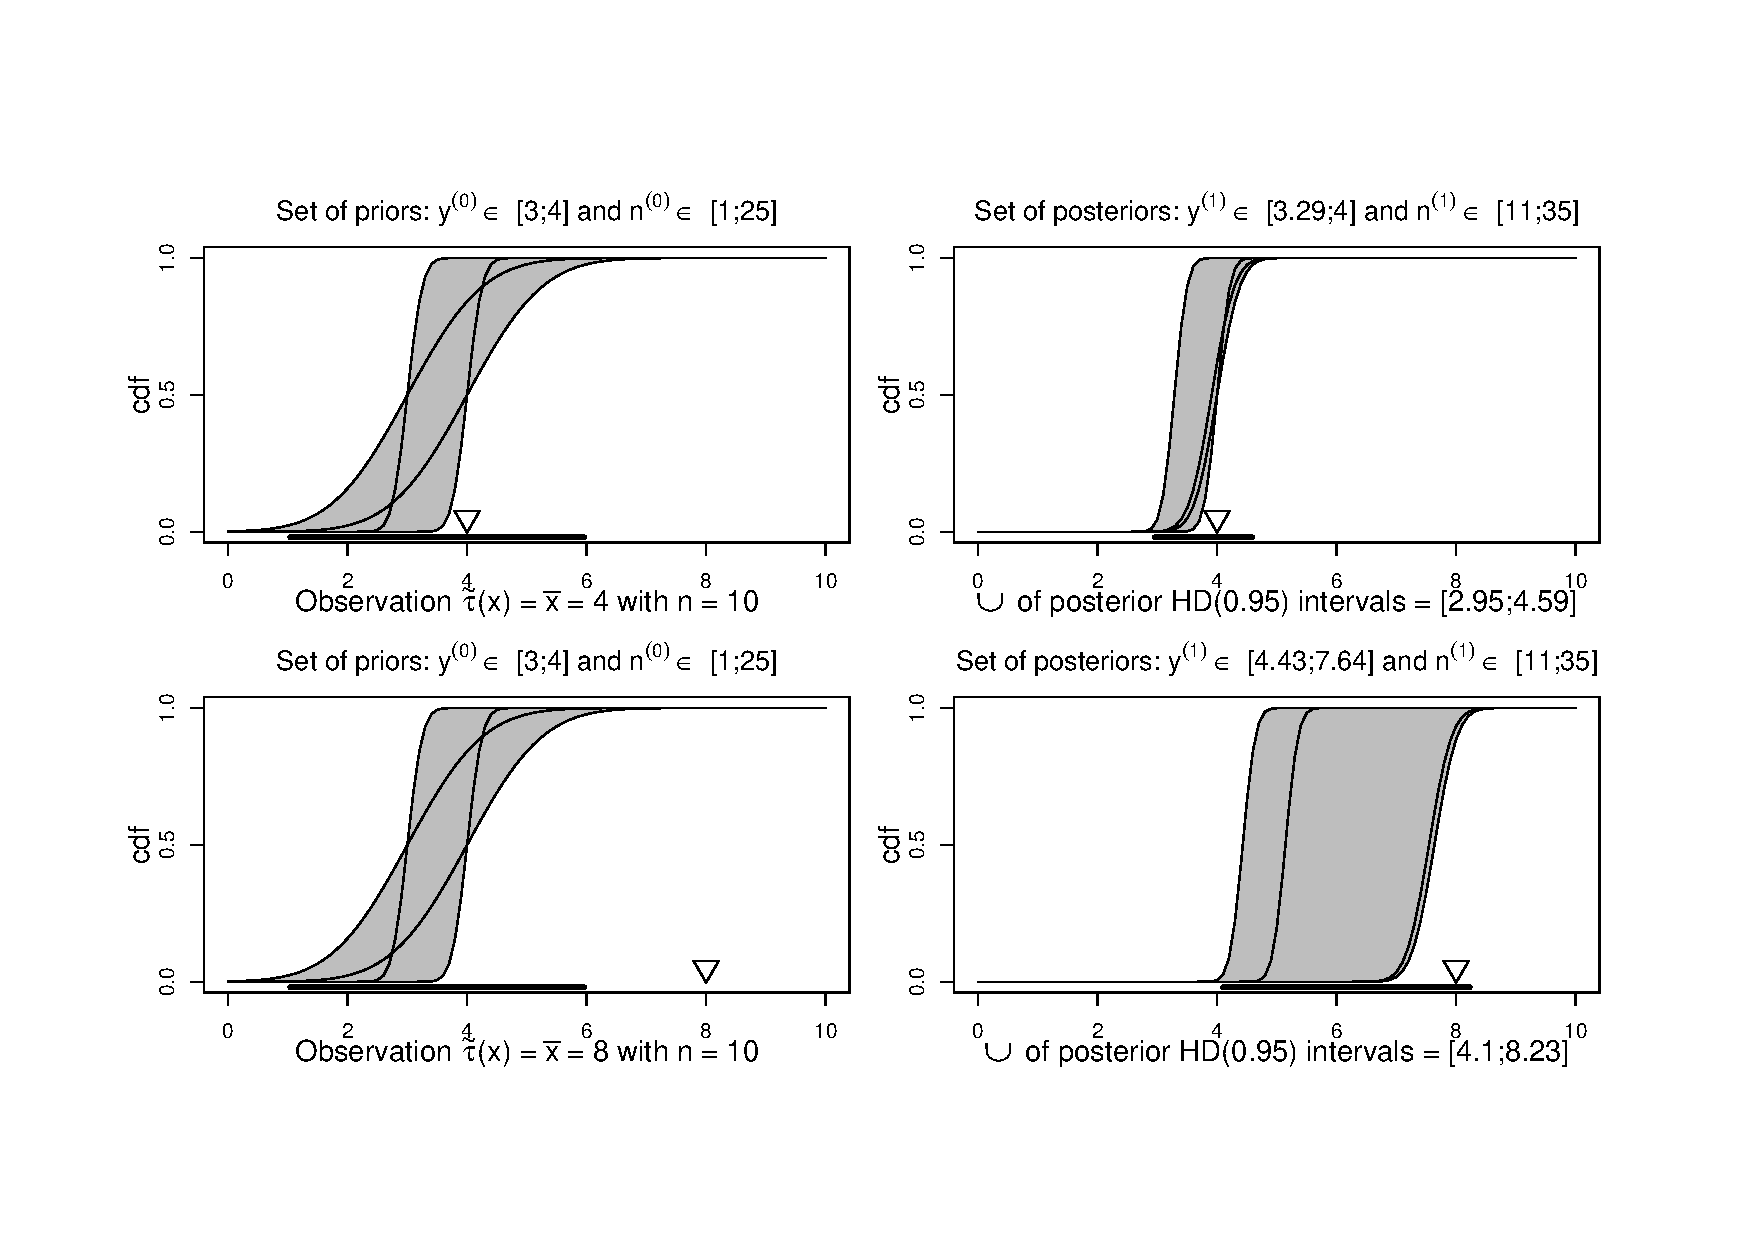
\includegraphics[trim = 20mm 20mm 20mm 25mm, clip, width=\textwidth]{figs/jstp-paper_nv_nvar_vertfu01_081128}};}
\end{tikzpicture}
\end{frame}

\begin{frame}{%General Framework for 
Canonical Exponential Families}
  Conjugate priors like the Beta can be constructed
  for sample distributions (likelihood) from:
  \begin{definition}[Canonical exponential family]
  \begin{equation*}
    f(x \mid \psi)=h(x)\exp\big\{\psib^T\tau(x) - \bpsib) \big\}
  \end{equation*}
  \vspace*{-2.5ex}
  \begin{itemize}
  \item includes multinomial, normal, Poisson, exponential, \dots
  \item $\psi$ generally a transformation of original parameter $\theta$
  \end{itemize}
  \pause
  \end{definition}
  \vspace*{-0.5ex}
  \begin{definition}[Family of conjugate priors]
  A family of priors for i.i.d.\ sampling from the can.\ exp.\ family:
  \begin{equation*}
    f(\psib\mid\nzg,\yzr)
    \propto \exp\big\{ \nzg \big[\psib^T \yzr - \bpsib\big]\big\}
  \end{equation*}
  with hyper-parameters $\nzg$ and $\yzr$.
  \end{definition}
\end{frame}

\begin{frame}
    \end{equation*}
    where
    \begin{align*}
      \vec{x} &= (x_1,\dots,x_n) &
      \tau(\vec{x}) &= \sum_{i=1}^n \tau(x_i) \\
      \nng &= \nzg + n &
      \ynr &= \frac{\nzg}{\nzg + n} \cdot \yzr + \frac{n}{\nzg + n} \cdot \frac{\tau(\vec{x})}{n}
    \end{align*}
  \end{theorem}
\begin{itemize}
\item $\yzr$ = \alert{prior expectation} of $\tau(\vec{x})/n$
\item $\nzg$ determines \alert{spread} and \alert{learning speed}
\end{itemize}
\end{frame}

\iffalse
\begin{frame}{%General Framework for 
IP with Canonical Exponential Families}
%\pause
\begin{itemize}
\item usefulness of this framework for IP / robust Bayes\\ discovered by \textcite{2005:quaeghebeurcooman} %Quaghebeur \& de Cooman
\item near-noninformative sets of priors\\ developed by Benavoli and Zaffalon \parencite*{2012:benavolizaffalon,2015:benavolizaffalon}
\item for informative sets of priors, \textcite{2009:WalterAugustin} %Walter \& Augustin
  suggest to use parameter sets $\PZ = [\nzlg,\nzug] \times [\yzlr, \yzur]$
\end{itemize}
\end{frame}
\fi

\begin{frame}{General Model Properties}
\uncover<1->{%
Good inference properties} %\hyperlink{othermodels-app}{\small (cf.\ other models based on sets of priors)}}
\begin{itemize}%[<+->]
%\note<10>[item]{In contrast to other models based on sets of priors,\\
%this model is easy to handle and to elicit,\\ and has very favourable inference properties}
\item<1-> $n \to \infty$\hspace*{1.6ex}%
%\uncover<2->{\then\ \ $\ynr$ values in $\PNc \to \frac{\tau(\x)}{n}$\hspace*{0.9ex}}%
%\uncover<3->{\then\ \ `Bayesian consistency'}
\uncover<2->{\play\ $\ynr$ stretch in $\PNc \to 0$\hspace*{1.6ex}}%
\uncover<3->{\play\ precise inferences}
%\item<4-> larger $\nzg$\hspace*{1.6 ex}\play\ larger $\PNc$ \hspace*{8.84ex}\play\ more vague inferences
%\note<10>[item]{larger $\nzg$ as compared to $n$:
%more weight on imprecise prior $\MZ$\\ leads to more imprecise posterior $\MN$}
\item<4-> larger range of $\yzr$ in $\PZc$\hspace*{1.6ex}\play\ larger range of $\ynr$ in $\PNc$\\[0.5ex]
\hspace*{30.02ex}\play\ more vague inferences
%\note<10>[item]{more imprecise prior $\MZ$ leads to more imprecise $\MN$}
\end{itemize}
\uncover<5->{%
Model very easy to handle:}
\begin{itemize}%[<+->]
\item<5-> Hyperparameter set $\PZc$ defines set of priors $\MZ$
\item<6-> Hyperparameter set $\PNc$ defines set of posteriors $\MN$
\item<7-> $\PZc \to \PNc$ is easy: $\nng = \nzg + n$, $\ynr = \frac{\nzg}{\nzg + n}\,\yzr + \frac{n}{\nzg + n}\cdot\frac{\tau(\x)}{n}$
%\item<9-> For quantities linear in posteriors, bounds are attained at ``pure'' posteriors $p(\psib\mid\nng,\ynr)$
%\then\ optimise over $\PNc$ (not over $\MN$)
\item<8-> Often, optimising over $(\nng,\ynr) \in \PNc$ is also easy:\\
\alert{closed form solution} for $\ynr$ = posterior `guess' for $\frac{\tau(\x)}{n}$ (think: $\bar{x}$)\\
when $\PZc$ has `nice' shape
\end{itemize}
\end{frame}

\frame{\frametitle{Hyperparameter Set Shapes}
%graphs line, rectangle, eggplant
\vspace*{-4ex}
\begin{tikzpicture}
%\uncover<1>{\node {\includegraphics[scale=0.75]{../R/shape0.pdf}};
%            \draw[-stealth,very thick] (-1,-0.4) -- (2.3,1.1) node [above,midway,sloped] {+ data};}
\uncover<1>{\node {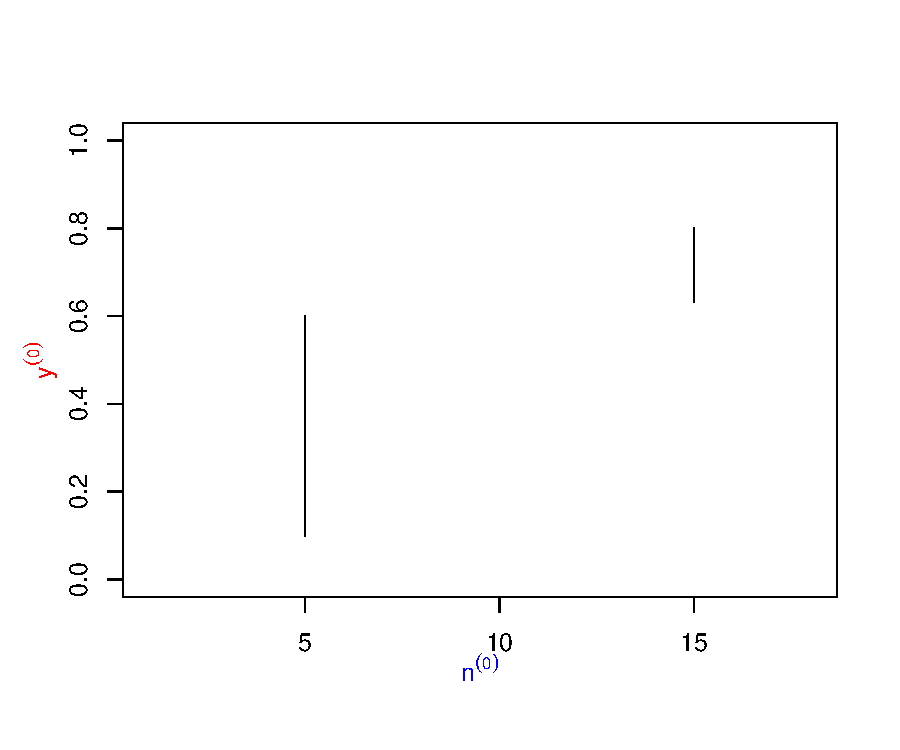
\includegraphics[scale=0.75]{figs/shape1}};
            \draw[-stealth,very thick] (-1,-0.4) -- (2.3,1.1) node [above,midway,sloped] {+ data};}
\uncover<2>{\node {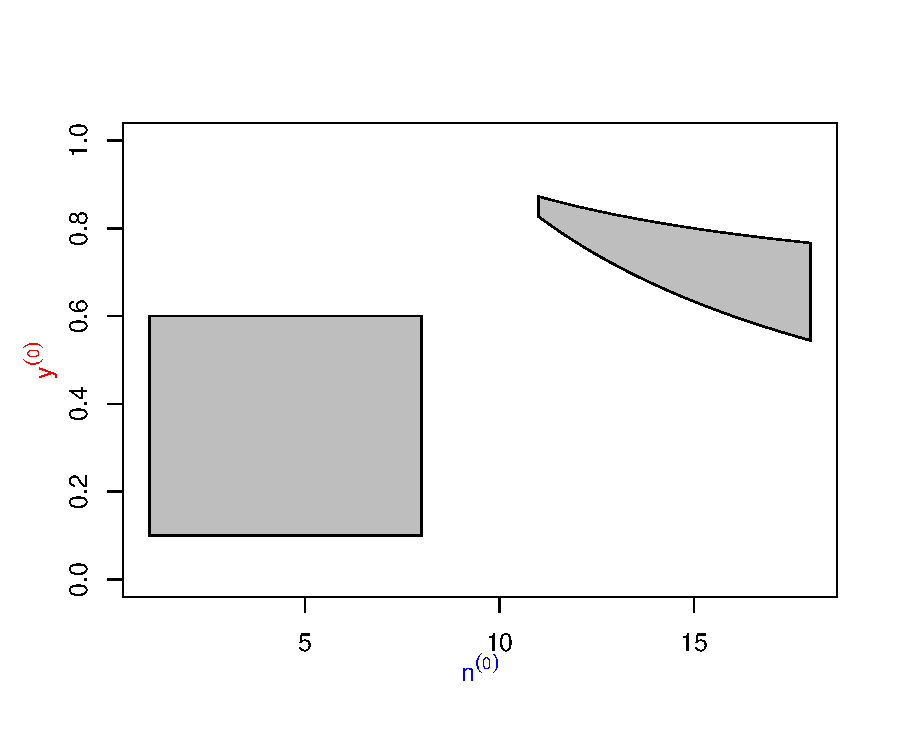
\includegraphics[scale=0.75]{figs/shape2}};
            \draw[-stealth,very thick] ( 0,-0.5) -- (2.3,1.1) node [above,midway,sloped] {+ data};}
\uncover<3>{\node {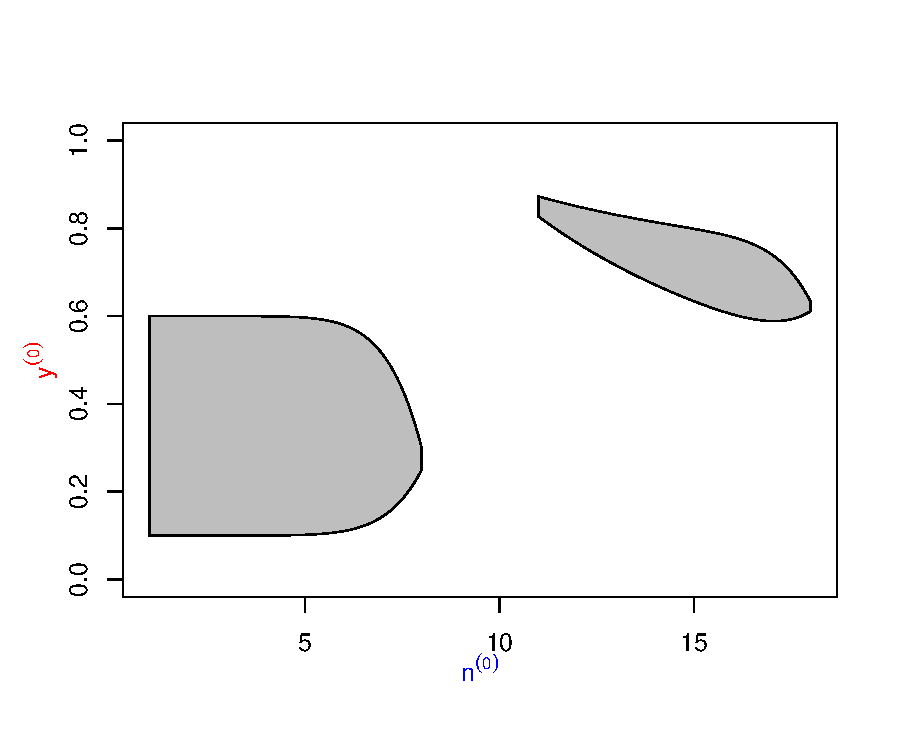
\includegraphics[scale=0.75]{figs/shape3}};
            \draw[-stealth,very thick] ( 0,-0.5) -- (2.3,1.1) node [above,midway,sloped] {+ data};}
\end{tikzpicture}
}

\begin{frame}{Hyperparameter Set Shapes}
\begin{itemize}%[<+->]
\item<1-> Set shape is crucial modeling choice:\\ %A range of $\nzg$ values is needed for \pdc\ reaction
trade-off between model complexity and model behaviour
% \begin{itemize}
\item<2-> $\PZc\! = \nzg \times [\yzlr, \yzur]$
 %{\small (Walley\,1996;\,Quaghebeur\,\&\,de\,Cooman\,2005)}:\\
 {\footnotesize \parencite{1996:walley::idm,2005:quaeghebeurcooman}:}\\
 $\PNc\! = \nng \times [\ynlr, \ynur]$ \play\ optimise over $[\ynlr, \ynur]$ only,\\
 \hspace*{20.9ex}but no prior-data conflict sensitivity
\item<3-> $\PZc\! = [\nzlg,\nzug] \times [\yzlr, \yzur]$ %{\small (Walley 1991; Walter \& Augustin 2009)}:\\
 {\footnotesize \parencite{1991:walley,2009:WalterAugustin}:}\\
 $\PNc$ have non-trivial forms (banana / spotlight), but prior-data conflict sensitivity and closed form for $\min / \max \ynr$ over $\PNc$\\
 implemented as \textsf{R} package \texttt{luck} {\footnotesize \parencite{luck-package}}
% For other inferences, \textbf{R} package \hyperlink{luck-app}{\texttt{luck}} implements optimisation
% over $\PNc$ via box-constraint optimisation over $\PZc$
% \end{itemize}
\item<4-> Other set shapes possible, but may be more difficult to handle %elicit
%\item<8-> Prior information may be such that range of $\yzr$ changes with $\nzg$ (or vice versa)
\end{itemize}
\end{frame}

\begin{frame}{Hyperparameter Set Shapes}
%\hspace*{-2ex}%
%\uncover<2->{%
%\vspace*{-7ex}%
%\begin{center} %trim=l b r t
\vspace*{2ex}%
set shape for strong prior-data agreement {\small \parencite{ipmu2016}} %[A.2]{2013:diss-gw}}
\begin{tikzpicture}
%\includegraphics[trim = 40mm 35mm 40mm 45mm, clip, width=\textwidth]{../R/boatshape-durham0913} % width=8, height=6
\uncover<1>{\node {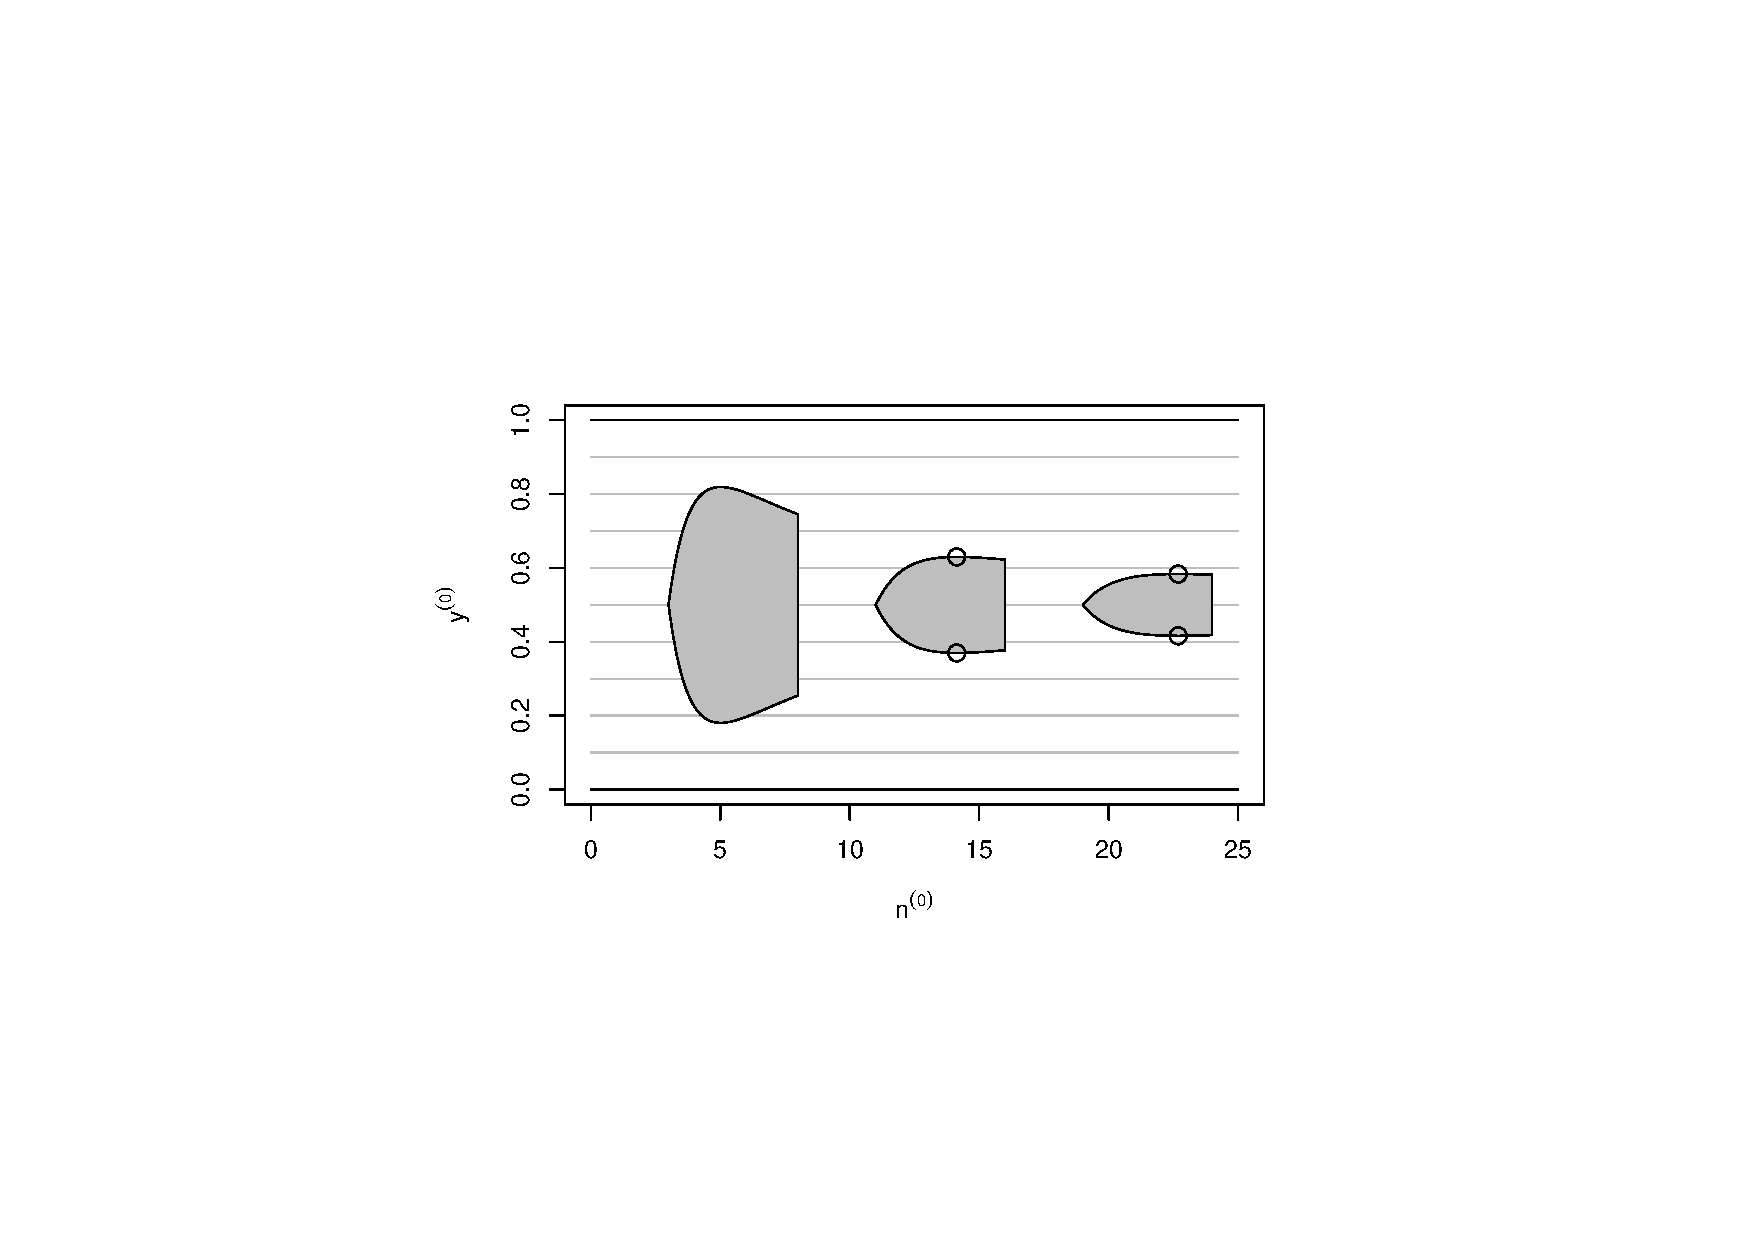
\includegraphics[trim = 70mm 52.5mm 70mm 65mm, clip, width=\textwidth]{figs/boatshape-defense-1}};} % width=6, height=4.5
\uncover<2>{\node {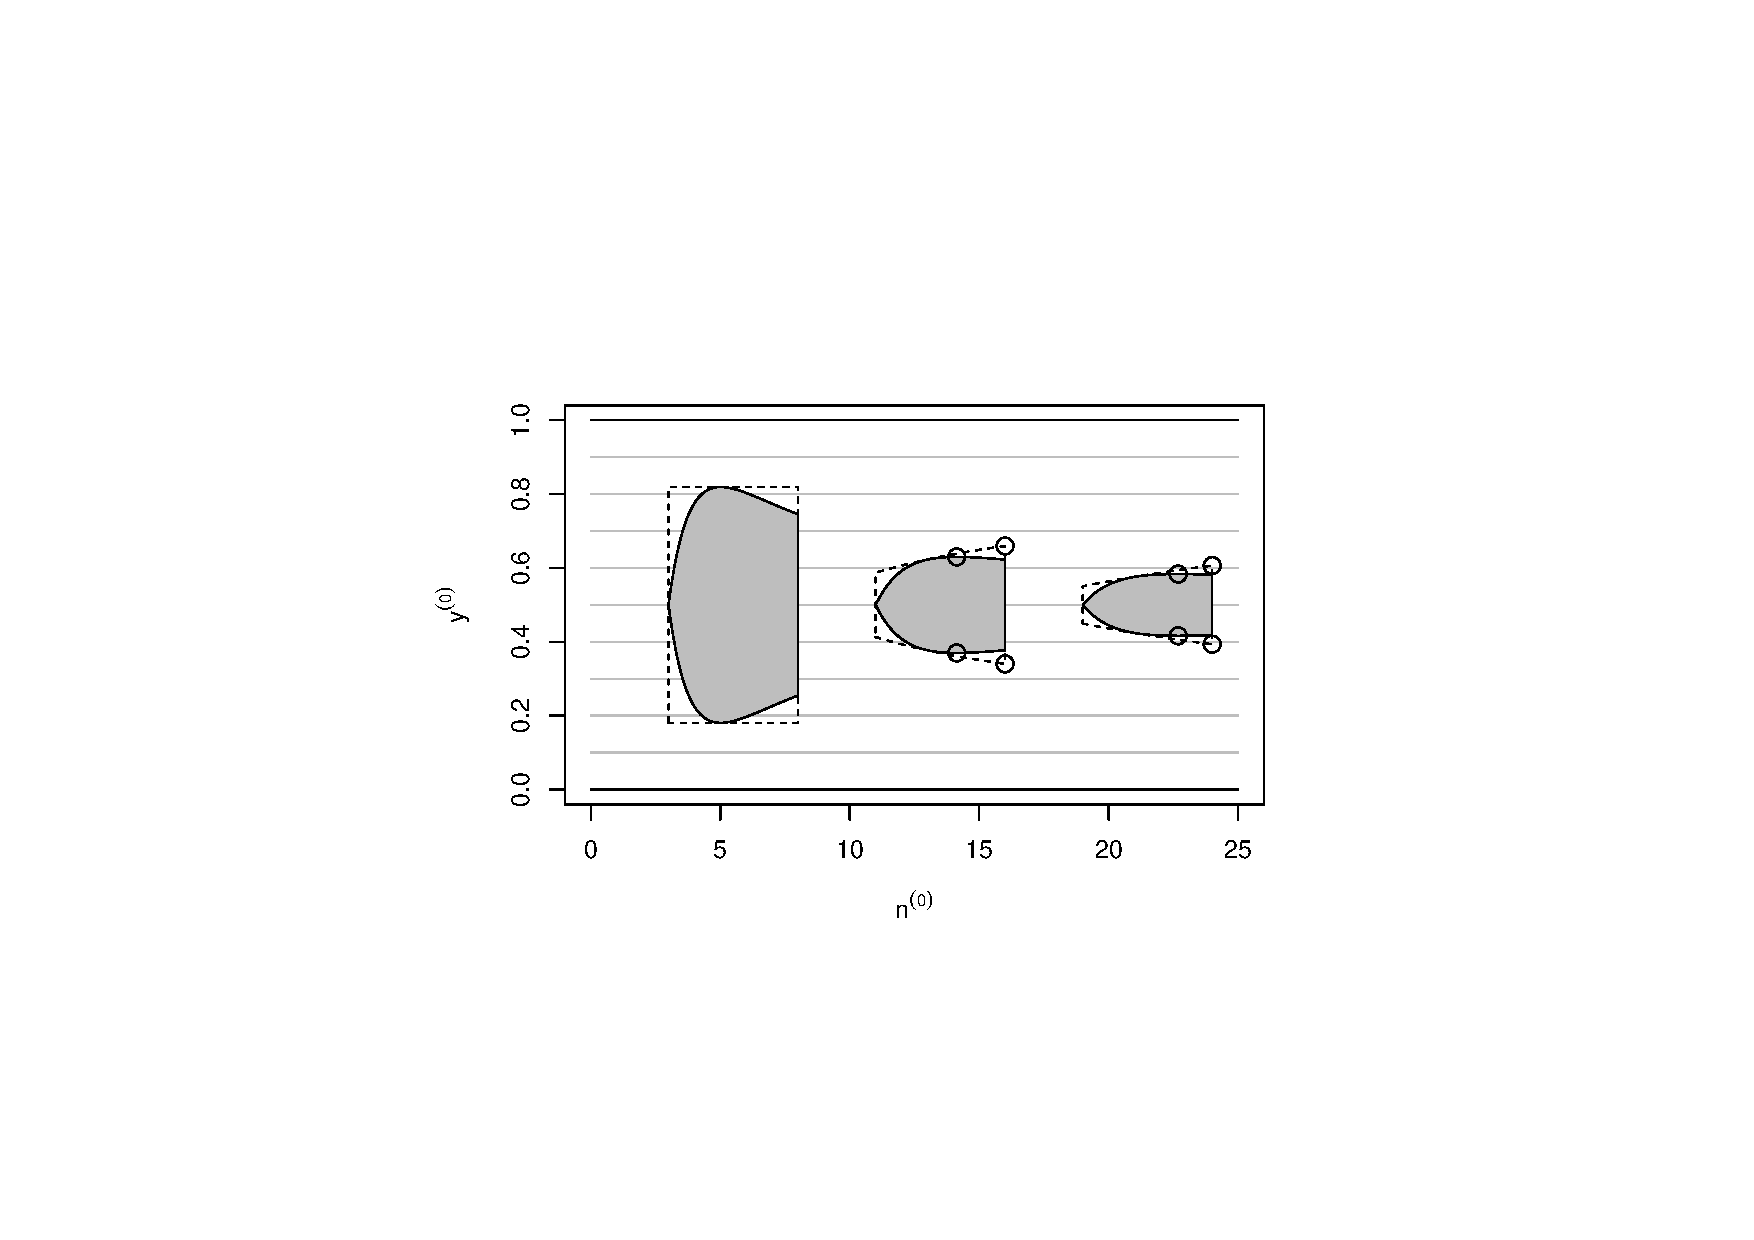
\includegraphics[trim = 70mm 52.5mm 70mm 65mm, clip, width=\textwidth]{figs/boatshape-defense-2}};} % width=6, height=4.5
\end{tikzpicture}
%
%\end{center}%}
\end{frame}

\begin{frame}{Robust Bayesian Analysis: Other Models}
\begin{itemize}
\item How to define sets of priors $\MZ$ is a crucial modeling choice
\item Sets $\MZ$ via parameter sets $\PZ$ seem to work better than other models discussed in the robust Bayes literature:
\begin{itemize}
\item Neighbourhood models
\begin{itemize}
\item set of distributions `close to' a central distribution $P_0$
\item example: $\varepsilon$-contamination class:
$\{ P : P = (1-\varepsilon) P_0 + \varepsilon Q, Q \in \mathcal{Q} \}$\\
\quad\play\ not necessarily closed under Bayesian updating
\end{itemize}
\pause
\item Density ratio class / interval of measures 
\begin{itemize}
\item set of distributions by bounds for the density function $f(\vartheta)$:
\begin{align*}
\mathcal{M}\uz_{l,u} = \big\{ f(\theta) :
\exists c \in \posreals: l(\theta) \le c f(\theta) \le u(\theta)\big\}
\end{align*}
\item posterior set is bounded by updated $l(\theta)$ and $u(\theta)$
\item $u(\theta)/l(\theta)$ is constant under updating\\
\quad\play\ size of the set does not decrease with $n$\\
\quad\play\ very vague posterior inferences
\end{itemize}
\end{itemize}
\end{itemize}
\end{frame}

\begin{frame}{Summary}
  \begin{itemize}%[<+->]
%  \item *** parametric distributions often chosen for tractability / convenience (Normal vs Cauchy!)
  \item choice of prior can severely affect inferences \\
    even if your prior is `non-informative'
  \item solution: go imprecise %systematic sensitivity analysis over prior parameters
  \item models from canonical exponential family make this easy to do
    %{\footnotesize \parencite{2005:quaeghebeurcooman,2012:benavolizaffalon,2015:benavolizaffalon}}
    {\footnotesize (\cite{2005:quaeghebeurcooman}; Benavoli and Zaffalon \cite*{2012:benavolizaffalon,2015:benavolizaffalon})}
  \item allows to adequately express the quality of prior information
%  \item a.k.a.\ parametric p-box 
  \item close relations to robust Bayes literature\\
    {\footnotesize \parencite{1994:berger,2000:rios}} %,2005:ruggeri}}
  \item concerns uncertainty in the prior\\
    {\footnotesize (uncertainty in data generating process: imprecise sampling models)}
%  \item here: focus on imprecise Dirichlet model
  \item if your prior is informative then prior-data conflict can be an issue
    {\footnotesize \parencite{2009:WalterAugustin,2013:diss-gw}}
%    (we'll come back to this in the system reliability talk)
  \end{itemize}
\end{frame}

\begin{frame}[allowframebreaks]{References}
%\begin{frame}[allowframebreaks]{References}
%
%  \bibliographystyle{plain}
%  {\scriptsize
%  \bibliography{../_diss/v1/bib/other-refs,../_diss/v1/bib/itip-refs} 
%  }
\printbibliography[heading=none]
\end{frame}

\end{document}
